\documentclass[oneside]{utmthesis}
% Options
% Size [a4draft, b5final]
% Language [english, malay]
% Printing [twoside, oneside]
% Default option [a4draft, english, twoside]

\usepackage{graphicx}
\usepackage{url} 
\usepackage{pdflscape}
\usepackage{longtable}
\usepackage{notoccite}
\usepackage[numbers]{natbib}
\usepackage{multirow}%
\usepackage{algorithm}
\usepackage{algpseudocode}
\usepackage{array}%
\usepackage{color,soul}%
 \usepackage[table,xcdraw]{xcolor}


\usepackage{booktabs}
\usepackage[caption=false]{subfig}
\newcolumntype{P}[1]{>{\centering\arraybackslash}m{#1}}%

%This is to make sure vertical spacing non-stretchable
\raggedbottom


% Required information
\title{LexiFlow: A Web Platform for Translating and Transcribing Native Mandarin Content}

\author{Adam Ismail Hassan Amer Abouraya}
% \metricno{A22EC0002}
% \dob{26 July 2025}
\degree{Bachelor of Computer Science}
\specialization{Software Engineering}
\intakeyear{2022}
\faculty{Faculty of Computing}
\titledate{July 2025}
% \titleyear{2025}
% \semester{2024/2025-2}
% \signingdate{25 June 2025}

\award{1}

\superone{Dr.~Shahliza Binti Abd Halim}




\begin{document}


% ----------------------------------------------------------------
% \coverpage
% \superpage
% 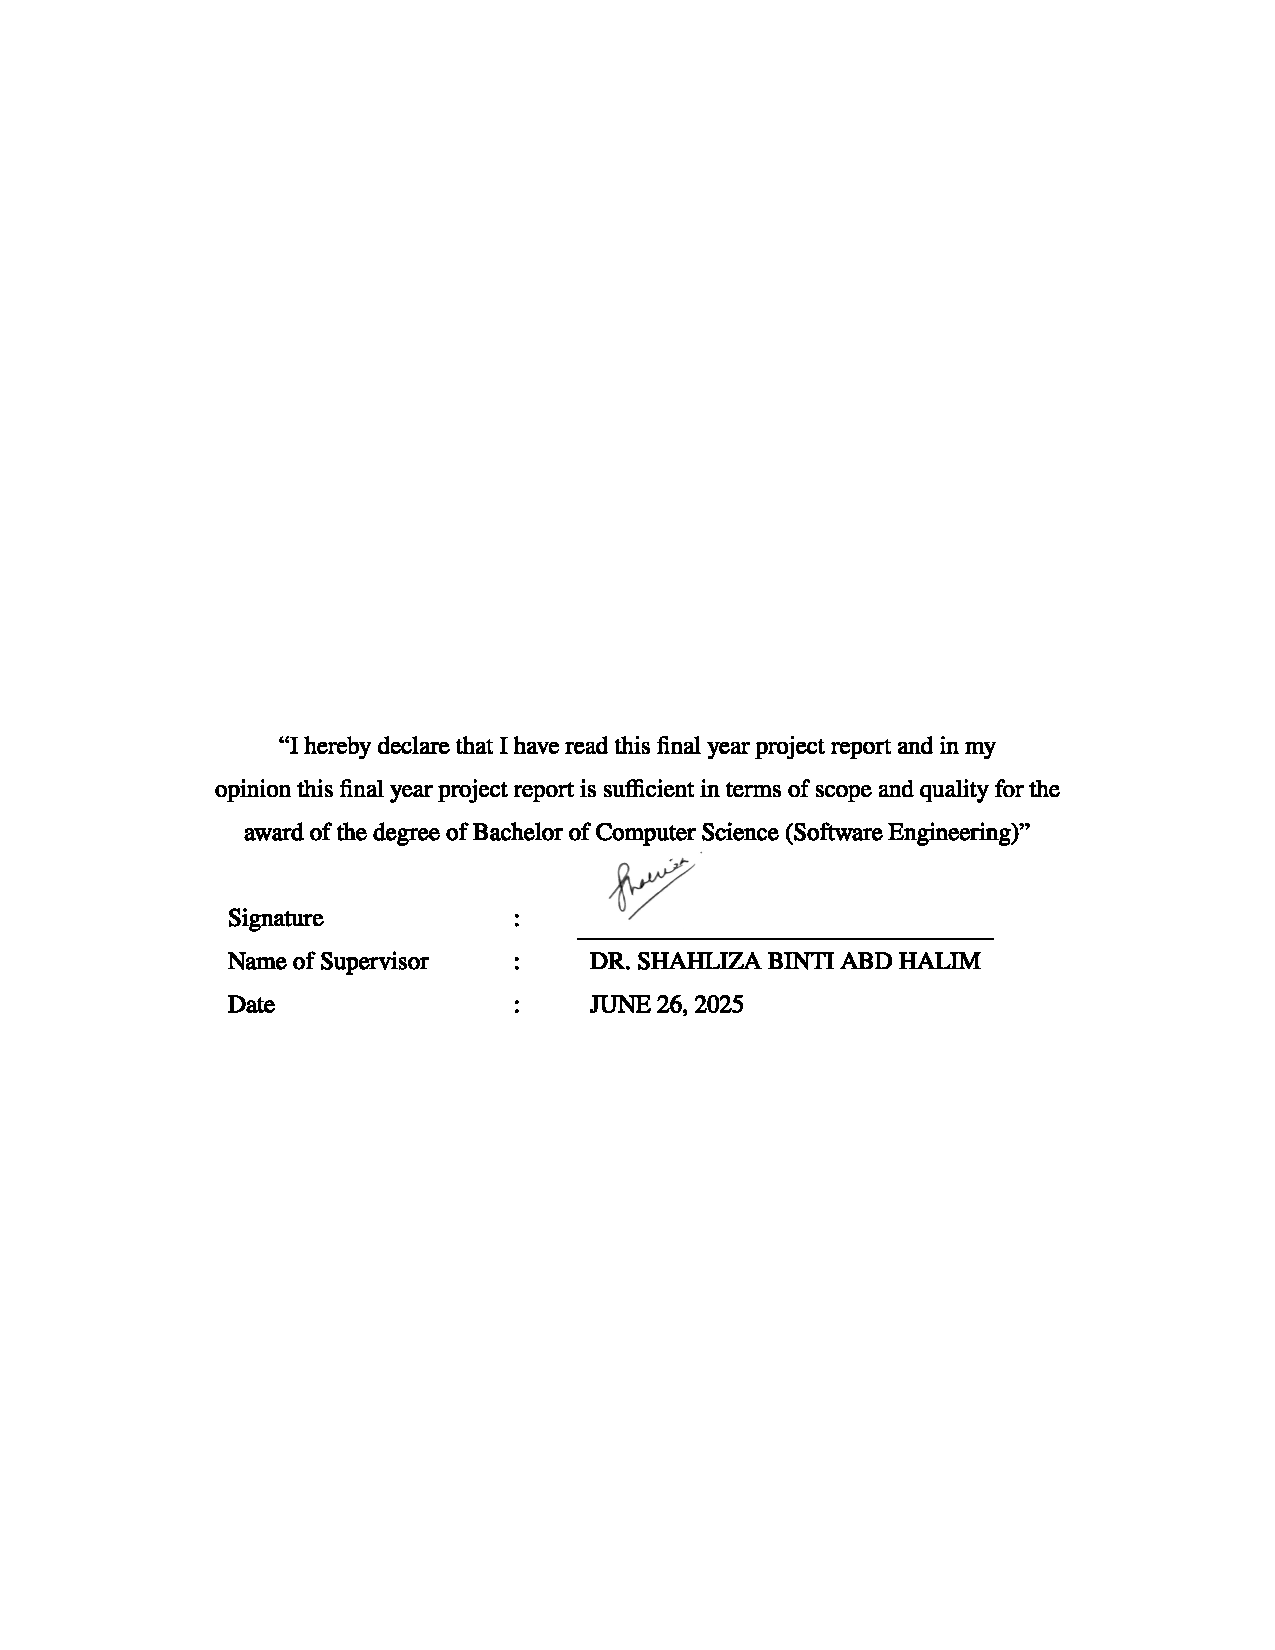
\includepdf[pages=1]{./figs/super2.pdf}
% \certification

% \frontmatter
% \maketitle
% \declaration

\normalsize
% ----------------------------------------------------------------

% \begin{dedication}
%     This thesis is dedicated to my father, who taught me that the best kind of knowledge to have is that which is learned for its own sake. It is also dedicated to my mother, who taught me that even the largest task can be accomplished if it is done one step at a time.\
% \end{dedication}

% \begin{acknowledgement}
%     In preparing this thesis, I was in contact with many people, researchers, academicians, and practitioners. They have contributed towards my understanding and thoughts. In particular, I wish to express my sincere appreciation to my main thesis supervisor, Dr. Shahliza Binti Abd Halim, for encouragement, guidance, critics and friendship. Without her continued support and interest, this thesis would not have been the same as presented here.

%     My fellow students should also be recognised for their support. My sincere appreciation also extends to all my colleagues and others who have provided assistance at various occasions. Their views and tips are useful indeed. Unfortunately, it is not possible to list all of them in this limited space. I am grateful to all my family members.
% \end{acknowledgement}

% \begin{abstract}
%     LexiFlow addresses the critical challenge of making authentic Mandarin content accessible and comprehensible for language learners. Traditional methods for creating learning materials are labor-intensive, requiring manual transcription, translation, and annotation, which limits the availability of engaging resources. Existing platforms often depend on pre-existing subtitles and lack support for Mandarin-specific features such as pinyin and sentence-level segmentation. LexiFlow is a web-based platform that automates the processing of Mandarin audio and video by leveraging advanced voice activity detection, automatic speech recognition, neural machine translation, and pinyin generation. The system segments content into linguistically meaningful units, generates synchronized bilingual subtitles with pinyin, and stores processed materials in a searchable database for instant reuse. This approach reduces the workload for educators, expands the library of authentic content, and provides learners with accurate, time-aligned transcriptions and translations. LexiFlow’s modular, pipe-and filter architecture ensures scalability and maintainability, while its user-driven content model fosters personalized learning. It is hoped that the development of LexiFlow can demonstrate the feasibility and effectiveness of integrating state-of-the-art language technologies to enhance Mandarin language acquisition through real-world content.
% \end{abstract}

% \begin{abstrak}
%     LexiFlow menangani cabaran kritikal untuk menjadikan kandungan Mandarin tulen boleh diakses dan difahami oleh pelajar bahasa. Kaedah tradisional untuk mencipta bahan pembelajaran adalah intensif buruh, memerlukan transkripsi manual, terjemahan dan anotasi, yang mengehadkan ketersediaan sumber yang menarik. Platform sedia ada selalunya bergantung pada sari kata sedia ada dan kekurangan sokongan untuk ciri khusus Mandarin seperti pinyin dan pembahagian peringkat ayat. LexiFlow ialah platform berasaskan web yang mengautomasikan pemprosesan audio dan video Mandarin dengan memanfaatkan pengesanan aktiviti suara lanjutan, pengecaman pertuturan automatik, terjemahan mesin saraf dan penjanaan pinyin. Sistem membahagikan kandungan ke dalam unit yang bermakna dari segi bahasa, menjana sari kata dwibahasa yang disegerakkan dengan pinyin dan menyimpan bahan yang diproses dalam pangkalan data yang boleh dicari untuk digunakan semula segera. Pendekatan ini mengurangkan beban kerja untuk pendidik, mengembangkan perpustakaan kandungan tulen dan menyediakan transkripsi dan terjemahan yang tepat dan selaras masa kepada pelajar. Seni bina modular, paip dan penapis LexiFlow memastikan kebolehskalaan dan kebolehselenggaraan, manakala model kandungan dipacu penggunanya memupuk pembelajaran yang diperibadikan. Diharapkan pembangunan LexiFlow dapat menunjukkan kebolehlaksanaan dan keberkesanan penyepaduan teknologi bahasa terkini untuk meningkatkan pemerolehan bahasa Mandarin melalui kandungan dunia sebenar.
% \end{abstrak}

% ----------------------------------------------------------------
% \tableofcontents
% \listoftables
% \listoffigures
% ----------------------------------------------------------------
%List of abbreviation 
% \listofabbre
\addabbre{UTM}{Universiti Teknologi Malaysia}
\addabbre{NMT}{Neural Machine Translation}
\addabbre{ASR}{Automatic Speech Recognition}
\addabbre{VAD}{Voice Activity Detection}
\addabbre{HSK}{Hanyu Shuiping Kaoshi (Chinese Proficiency Test)}
\addabbre{API}{Application Programming Interface}
\addabbre{SQL}{Structured Query Language}
\addabbre{NoSQL}{Not Only SQL}

%List of symbols 
%\listofsymbols
%\addsymbol{$\gamma$}{gamma}

%Uncomment if have appendices
% \listofappendices

% ----------------------------------------------------------------

\mainmatter
\chapter{Introduction}
\section{Introduction}
Mandarin is not only a language but a powerful means to the future as it is spoken by more than one billion people and is gaining significant importance in business, technology and culture around the world. The growing importance of China as an economic power, leader in manufacturing and artificial intelligence and its increasing influence in the cultural arena opens doors to career opportunities in Mandarin. However, in the minds of many learners, the language is too complicated, both through its tonal pronunciation and through its complex characters, and mastering it seems impossible.

The studies in language acquisition have indicated that exposure to authentic content is the most effective way to learn a language~\citep{krashen1985,Mayer_2009}. Here authentic means that the material is genuine (real) and originally written for native speakers (books, movies, news articles, podcasts, conversations, etc.), not simplified or made-up for language learners. If students are interested in the materials they will be motivated and retaining more. This natural learning approach is consistent with children's first-language acquisition of language: immersion not memorization~\citep{cychosz2021, gowenlock2024}.

There are difficulties associated with many students using traditional methods. There is more focus on the rules of grammar than on exposure to natural language in textbooks and classrooms. While there are some applications available now that can assist with translation, there are difficulties with Mandarin. The character system does not help students because there is no similarity between the written characters and the sounds. Pinyin is available as a guide for pronunciation but is seldom used outside of school.

LexiFlow addresses these challenges by using a web platform which integrates sentence segmentation and machine translation models. The system receives audio and segments it into sentences and processes each one separately. This will help to increase accuracy and reduce the computing resource required. The system then keeps a repository of previously processed material so that content is not processed again and can be used to present to students, materials that are similar to their interests and abilities.
\section{Problem Background}

The lecturer of language at UTM has noticed a problem with the development of language among the students at UTM. A lot of students can learn the rules and vocabulary in their written exams, but having trouble with a real Mandarin conversation. This disparity between the student's performance in academics and the communication skills is a hindrance to the learning of the students. Authentic content will expose students to helpful vocabulary, natural speech patterns and culture that textbooks do not provide, particularly when linked with students' own interests to make the language more engaging.

The current method of producing Mandarin learning content is still time-consuming. Lecturers start by gathering authentic sources of audio or video. Often taking a lot of time to find appropriate content. After selection of content, teachers will manually transcribe the spoken Mandarin, add pinyin and translation to it. This process can take as long as 8-10 hours for a couple minutes of content and can put a significant strain on teachers.

These challenges are not met by existing solutions. The availability of YouTube subtitles is essential to popular platforms such as LanguageReactor, which is hard to find for Mandarin content compared to English content. As for general transcription services, for example the ones at Transcribe.com, they transcribe material without the time-stamped subtitle format that students find useful in mapping spoken sounds to written text, and they don't support pinyin, which is essential for Mandarin learners to learn how to pronounce the text.

Students need a system that effectively processes the authentic Mandarin content and shows both the spoken and written language. The solution should include accurate transcriptions and timings, pinyin pronunciation guides, and quality translations that link naturally spoken Mandarin with its written form.
\section{Project Aim}
Create a web platform called LexiFlow for processing, transcription and translation of authentic Mandarin content with the aid of advanced sentence-level segmentation and translation models. To assist students to grasp authentic Mandarin dialogues in real life.
\section{Project Objectives}\label{sec:obj}
The objectives of the project are:
\begin{enumerate}[label= (\alph*)]
    \item To identify and gather requirements from primary stakeholders, including language learners and educators.
    \item To design a web-based platform with a user interface and a database that provides synchronized, time-stamped bilingual subtitles.
    \item To develop a web platform based on stakeholder requirements, adding features such as audio/video processing, transcription, translation, and pinyin generation.
    \item To test and validate the platform using testing methodologies and domain expert's feedback to ensure accuracy in transcription, translation, and subtitle synchronization.
\end{enumerate}
\section{Project Scopes}
The scopes of the project are:
\begin{enumerate}[label= (\alph*)]
    \item The proposed platform will accept long-form audio or video input (up to 120 minutes) from user-uploaded files or YouTube URLs.
    \item The proposed platform will perform voice activity detection (VAD) and end-of-sentence detection to segment audio into linguistically meaningful sentence-level chunks.
    \item The proposed platform will generate transcriptions using automatic speech recognition (ASR) and translations via Neural Machine Transformer (NMT) model.
    \item The proposed platform will produce synchronized, timestamped bilingual subtitles with original language text, target-language translation and pinyin annotations by utilizing the transformer model.
    \item The proposed platform will store processed subtitles in a searchable database indexed by content identifiers (e.g., URLs) to enable instant reuse without reprocessing.
    \item The proposed platform will provide a web interface for uploading content, customizing subtitle outputs
\end{enumerate}
\section{Project Importance}
The LexiFlow project is significant as it seeks to improve the language learner's experience. LexiFlow will be able to address the issue of scarce resources from online platforms and lecturers. With integration of machine translation models for translation and transcription, LexiFlow will enable students to learn from content they are interested in learning from.
\section{Report Organization}
The thesis consists of five well-rounded chapters. Chapter 1 presents the project and provides background, purpose, objectives, scope, importance and structure of the report. Chapter 2 presents an extensive literature review on the current systems and technologies pertaining to speech recognition, translation model and user interface, and finally a comparison with the available market solutions.

The system development methodology is described in chapter 3 which highlights the selected software development life cycle, the reasons for the choice of method and the major systems development stages. Chapter 4 provides an in-depth exploration of requirements analysis and system design, covering functional requirements, non-functional requirements, database design, and user interface requirements, all aimed at guaranteeing usability and functionality.

In the last chapter (Chapter 5), the findings from the paper are summarized, the project outcomes discussed and recommendations made for improvements to further develop and extend the LexiFlow system. This structure allows for a very logical flow and development with a detailed discussion of all aspects of the project from conceptualization to implementation and evaluation.
\chapter{LITERATURE REVIEW}
\section{Introduction}
A literature review and technologies review have been conducted to review the existing literature and technologies relevant to the development of the lexiflow system. It begins with a review of theories and models of second language acquisition that are relevant to the design of any L2 learning material. It then underscores the problems associated with symbolic language and discusses the existing methods and systems in the area of language acquisition. The purpose of this literature review is to give a foundation of theory and to highlight gaps that LexiFlow is looking to fill.
\section{Theories of Second Language Acquisition}
\subsection{Krashen's Input Hypothesis}
LexiFlow is based on one of the main theories behind language learning, the Input Hypothesis~\citep{krashen1985}. The hypothesis is that language learning takes place when learners are exposed to comprehensible input. In this context, the term comprehensible input is defined as input material that is at just one step above the learner's current level (i+1). According to this theory, acquisition of grammatical structures occurs naturally when learners are exposed to them, without formal teaching. This is based on the way children learn their first language, hearing and engaging with language in context.

Let's imagine that the student is an HSK2 student who can deal with simple daily life conversations. Based on the "i+1" principle by Krashen, this learner learns language best when he/she reads or hears content at approximately HSK 3 level that presents new words and new patterns of use, but not too many, while still containing elements with which he/she is familiar.

{Table~{\ref{tab:hsk2}}} summarizes the vocabulary requirements for each HSK (Hanyu Shuiping Kaoshi) level, which is the standardized Chinese proficiency test. As shown, each level builds cumulatively on the previous one. For example, a student at HSK 2 has mastered 300 words in total, while HSK 3 requires knowledge of 600 words.

\begin{table}[h]
    \centering
    \caption{HSK 2.0 Vocabulary Requirements \citep{hsk2}}\label{tab:hsk2}
    \begin{tabular}{@{}lll@{}}
        \toprule
        \textbf{Current Level (i)} & \textbf{Vocabulary Size} & \textbf{Cumulative Words} \\
        \midrule
        HSK 1                      & 150 words                & 150 words                 \\
        HSK 2                      & 150 words                & 300 words                 \\
        HSK 3                      & 300 words                & 600 words                 \\
        HSK 4                      & 600 words                & 1,200 words               \\
        HSK 5                      & 1,300 words              & 2,500 words               \\
        HSK 6                      & 2,500 words              & 5,000 words               \\
        \bottomrule
    \end{tabular}
    \smallskip

\end{table}

Numerous studies have validated this theory. For example,~\citet{RODRIGO2004} demonstrated that extensive exposure to comprehensible input through reading resulted in significantly greater vocabulary acquisition compared to traditional instruction methods. Similarly,~\citep{krashen2017} found that students exposed to extensive comprehensible input outperformed those following traditional grammar-translation methods, even when tested on grammatical knowledge.

However for Mandarin, the challenge lies in the ability to find authentic content that is both engaging and comprehensible. Figure~\ref{fig:mandarin_dilemma} is a perfect example of the Mandarin learning dilemma that LexiFlow aims to solve. Here we see a YouTube video which can be labeled as comprehensible input, with Chinese characters displayed as subtitles at the bottom of the screen. Crucially, these subtitles lack any Pinyin pronunciation guide, rendering them inaccessible to beginner and intermediate learners who haven't yet mastered thousands of characters. In addition, the video is not tailored to any specific proficiency level, and the subtitles option is disabled, making the use of any current translation tools impossible.

Figure~\ref{fig:mandarin_pinyin} shows an example of proper subtitles, which are hand-made by a YouTube channel. However, this process is extremely time-consuming and labor-intensive, making it very rare and with very limited library.


\begin{figure}[ht]
    \centering
    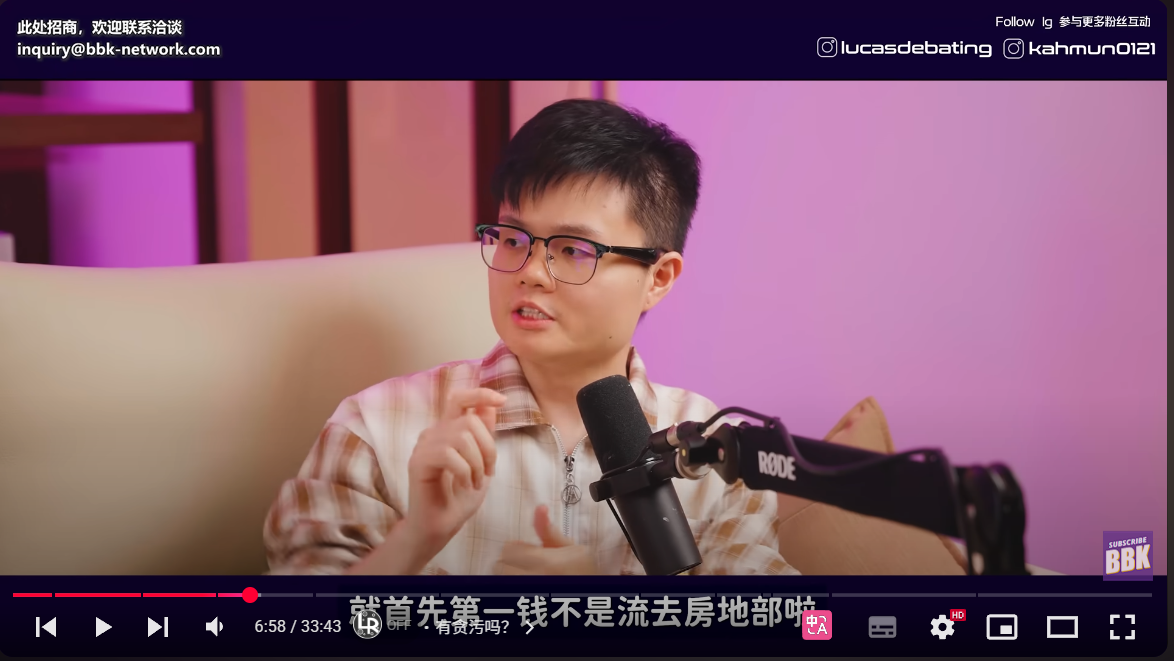
\includegraphics[width=0.8\textwidth]{./figs/yt.png}
    \caption{Example of Mandarin Learning Dilemma}
    \label{fig:mandarin_dilemma}
\end{figure}

\begin{figure}[ht]
    \centering
    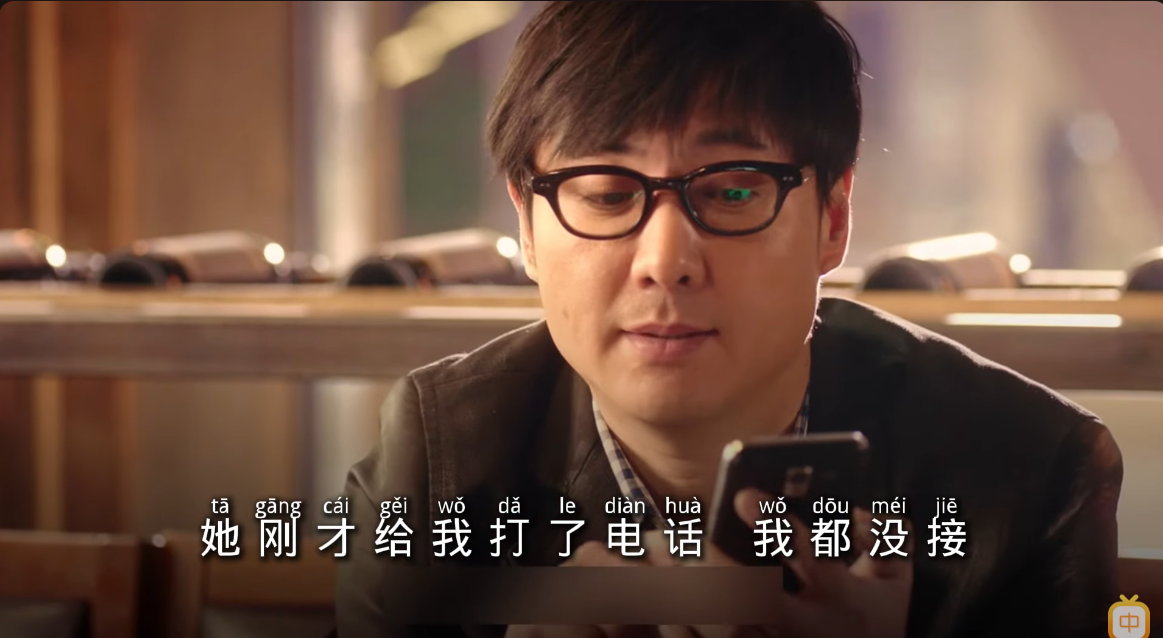
\includegraphics[width=0.8\textwidth]{./figs/yt2.png}
    \caption{Example of Proper Subtitles with Pinyin}
    \label{fig:mandarin_pinyin}
\end{figure}


\subsection{Multimedia Learning Theory}
Mayer's Multimedia Learning Theory~\citep{Mayer_2009} provides another crucial theoretical pillar for LexiFlow's approach. This theory proposes that people learn more deeply from words and pictures together than from words alone, particularly when the verbal and visual elements are presented simultaneously rather than successively.

\citet{jones2002} showed that students' vocabulary retention improved by 42\% when using both the visual and the written text, as opposed to learning from the written text alone. In character-based languages,~\citet{shen2010} concluded that a multimedia presentation that links spoken words, written characters and visual representations of the characters were more effective to recognize characters than the traditional method by 35\%.

In addition,~\cite{li2022} demonstrated that the Mandarin learners achieved higher scores on listening comprehension test when they were provided with subtitles for practice. It demonstrates their support for LexiFlow's strategy of multimodal inputs in their synchronization mode for transcription and translation.

\section{Challenges for Mandarin as Symbolic Language}
\subsection{Character Recognition and Sound Awareness}
Many learners are thrown a curve by the logographic system of writing used in Mandarin, as opposed to alphabetic writing systems, in which written symbols directly represent sounds. According to~\citet{everson2011} the number of times a western learner needs to see a Chinese character is 17 times before he or she can reliably recognize it while 8 exposures are enough for alphabetic language words. This added "mental load" is due to the visual complexity of the characters.

Since there is a gap between written and spoken Mandarin, linguists have termed it the `orthographic barrier'~\citep{shen2007}. This obstacle essentially hinders learning effectiveness, while students can understand spoken vocabulary, they are unable to relate them with written forms. As a stepping stone to this change, pinyin has become an important tool, but ~\citet{ye2013} noted that 76\% of intermediate learners still experienced problems in accessing character-only materials without the aid of pinyin.

LexiFlow overcomes this difficulty by keeping the important link between the sounds, pinyin and characters for authentic content, enabling learners to slowly develop their ability to recognize characters while also working with phonological representations to access meaningful content.

\subsection{Tonal Perception and Production}
Another major difficulty in the literature noted is Mandarin's tonal quality. Wang~\cite{wang1999} has shown that adult learners from non-tonal language backgrounds need special training to make the accurate perception and production of Mandarin's four tones. They found that beginners' accuracy in understanding the tones was still under 40 percent after 200 hours of classroom learning, without explicit training.

Tone is typically handled in textbooks by isolated examples or in perfectly prepared dialogues. These methods are unnatural ways to speak the language. LexiFlow offers opportunities for students to develop their tonal awareness. The content is authentic with pinyin annotations, with tone markers.

\section{Current System Analysis}
The model in which students learn from authentic content is facing great difficulties both for students and teachers. The current process is observed in UTM and interviews with Mandarin language teachers, which needs a lot of manual effort and has limited content library.
\subsection{Problem with Current System}
Current practice in embedding authentic Mandarin content into learning is very labour intensive, resource intensive and has limited quantity and quality of authentic materials available. The process as it is today (AS-IS) starts with either the instructors or motivated students looking for potentially suitable authentic content (as illustrated in the AS-IS swimlane diagram {Figure {\ref{fig:as_is}}}). The search process is time consuming and may return content that is not sufficiently levelled to meet the language proficiency requirements.

\begin{figure}[ht]
    \centering
    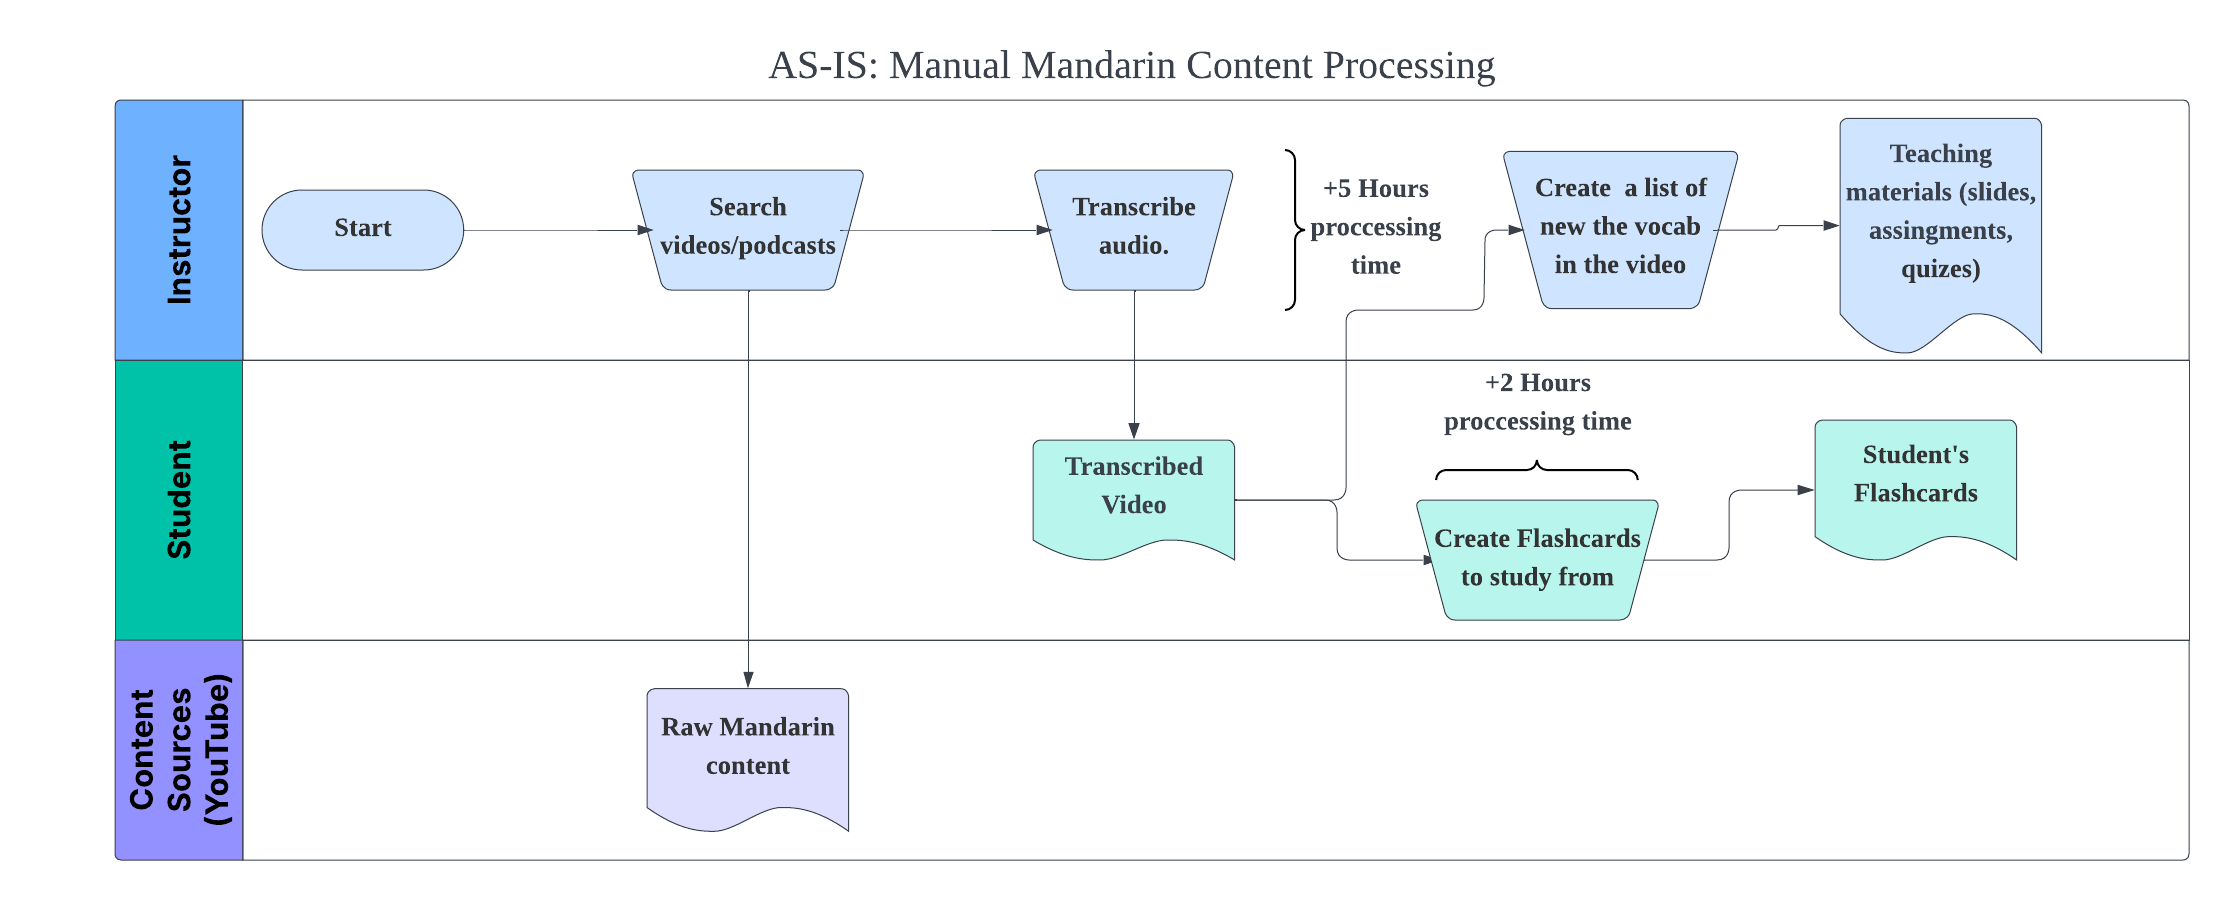
\includegraphics[width=1\textwidth]{./figs/AS-IS.PNG}
    \caption{AS-IS Swimlane Diagram}
    \label{fig:as_is}
\end{figure}

After content is identified, the real challenges start. The Mandarin audio must be manually transcribed and instructors have to make pinyin annotation and translation, which may take 8-10 hours for a 5-minute video. The volume of transcription work required makes it very difficult to provide a lot of content to students. If students are trying to go through this process alone, there are more obstacles to their understanding because there is no instant feedback.

The resulting materials are often likely to be without synced timelines that would enable learners to link the spoken and written words together. In addition, much of the material is rarely presented in context that would make it accessible to more intermediate students, and the material is often used at a level that only more advanced students are able to access.
\subsection{Proposed Solution}
LexiFlow solves these inefficiencies by using technology to automate the most time-intensive parts of content processing, all without compromising quality. The proposed system is designed to simplify the workflow, allowing both instructors and students to make full use of it ({Figure {\ref{fig:to_be}}}).

\begin{figure}[ht]
    \centering
    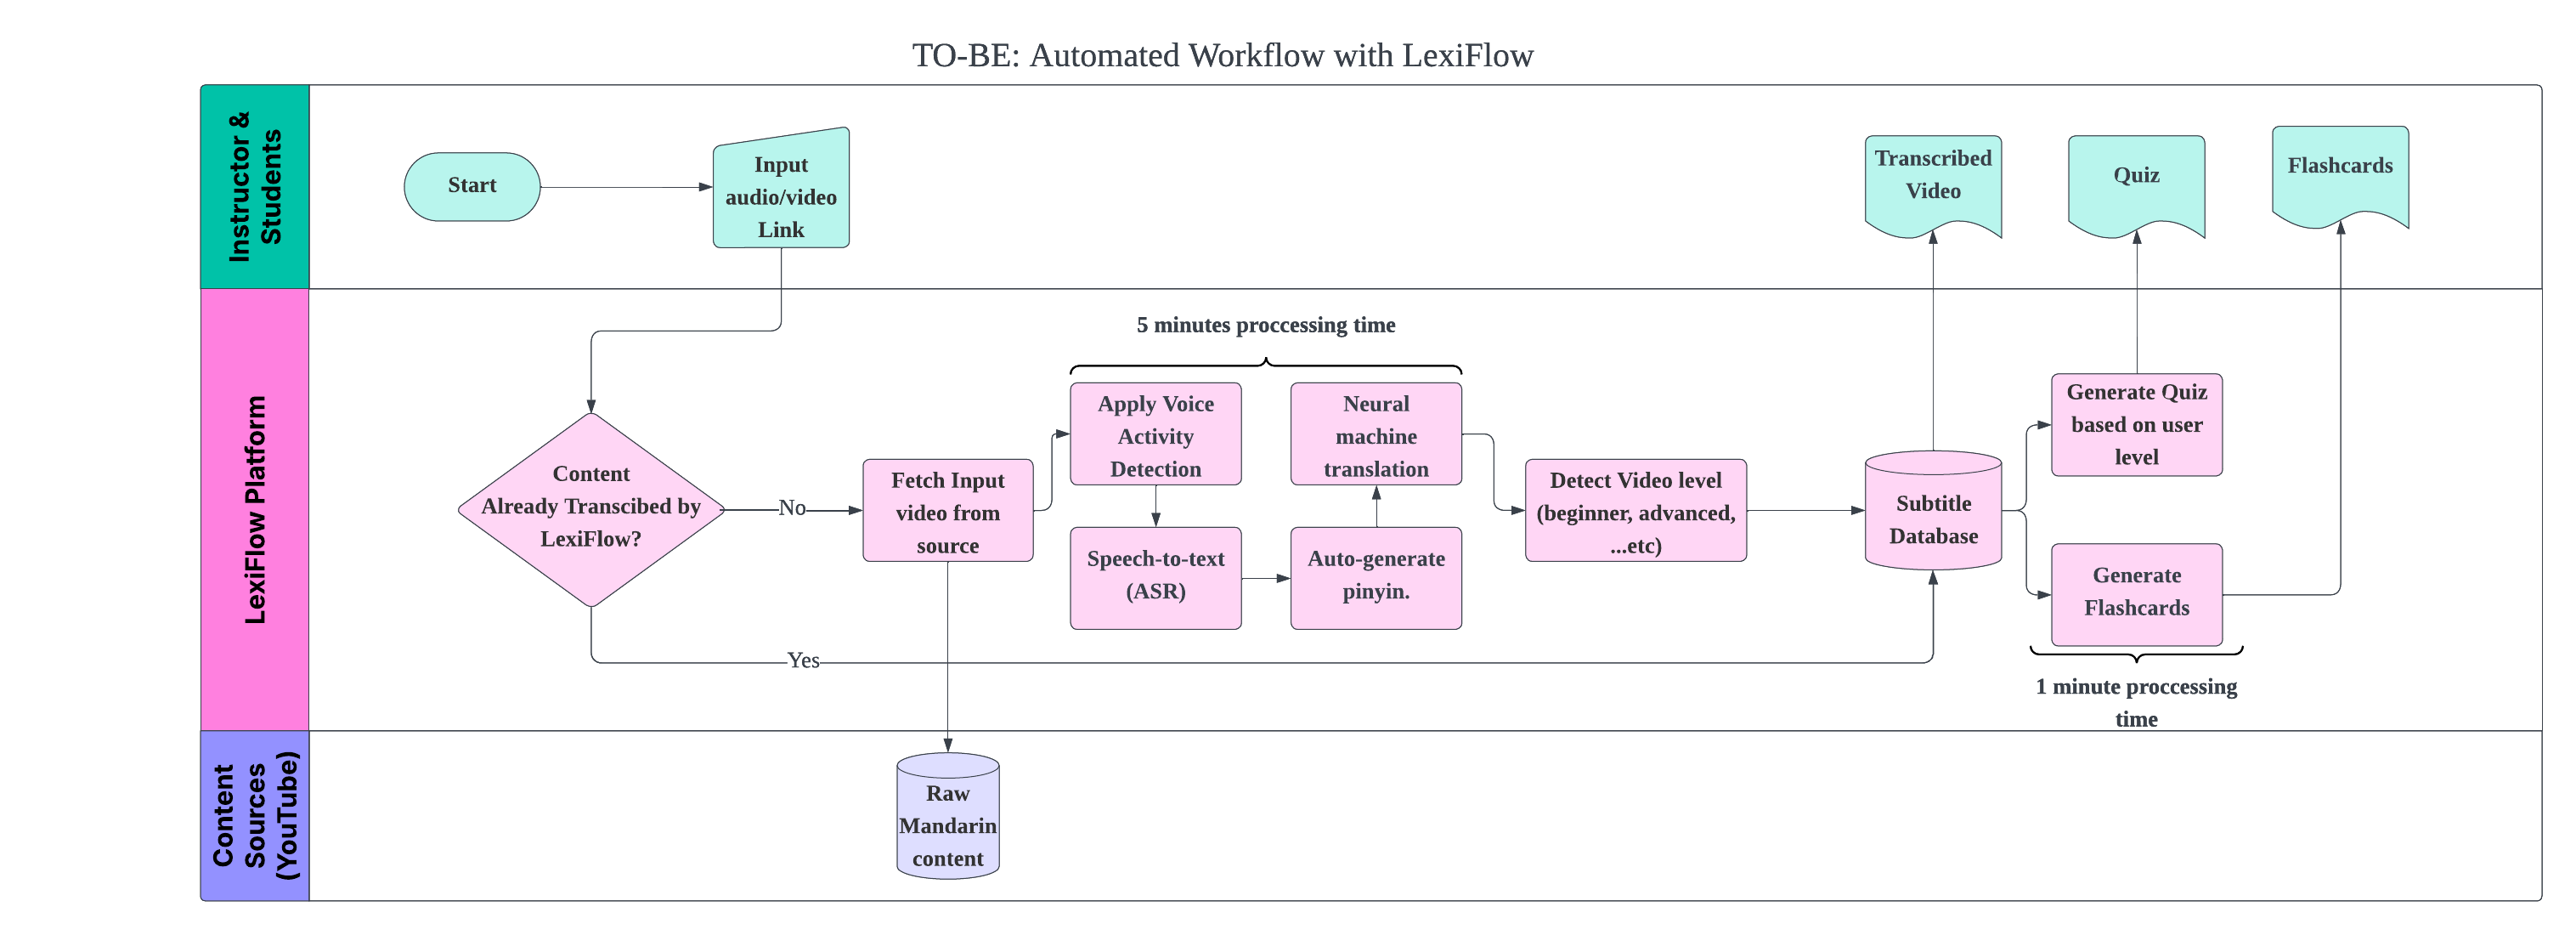
\includegraphics[width=1\textwidth]{./figs/TO-BE.PNG}
    \caption{TO-BE Swimlane Diagram}
    \label{fig:to_be}
\end{figure}



The process starts from the users submitting their actual Mandarin audio or video material to the platform. Each section of text is then automatically divided into smaller sentence level units, using voice activation detection algorithms, by LexiFlow. All the segments are separately transcribed by automatic speech recognition (ASR), then converted to pinyin and then translated into English by neural machine translation (NMT).

All processed material is stored in an indexed database which means that the same processed material doesn't need to be processed again if many users are accessing the same content. This allows for a growing ecosystem of content that becomes self-serving and expands according to user interests and needs.
\subsection{Comparison of Similar Video-Based Learning Platforms}
There have been a number of attempts to employ video in the learning of a foreign language, each with varying degrees of success. As shown by \citet{xu2020} who analyzed FluentU, the video libraries selected with interactive transcripts proved to be more effective in boosting listening fluency than audio exercises. Yet, the study also revealed a lack of content as a barrier, and advanced learners voiced complaints of lack of variety of content. The FluentU video browser, as seen in Figure~\ref{fig:fluentu-browse}, shows the platform's library of videos curated by FluentU. The video is shown in Figure~\ref{fig:fluentu} with interactive transcripts and words of interest.

\begin{figure}[H]
    \centering
    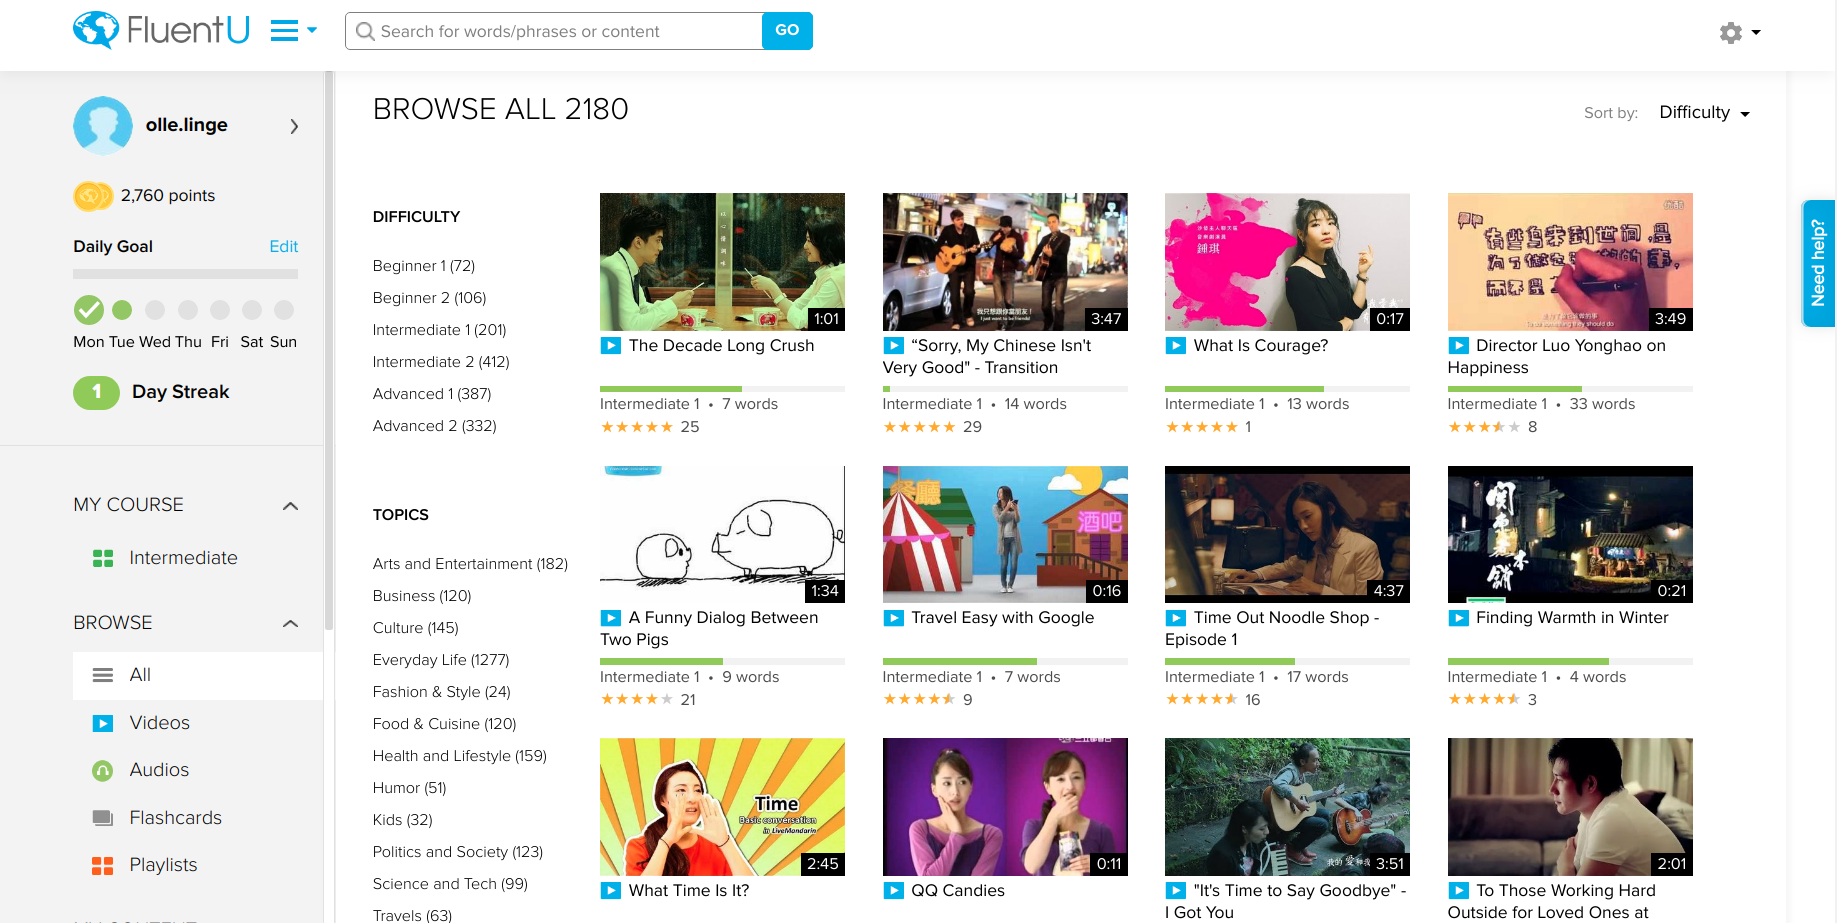
\includegraphics[width=1\textwidth]{./figs/fluentu-video-browse.png}
    \caption{FluentU Platform Video Browse Page}
    \label{fig:fluentu-browse}
\end{figure}

\begin{figure}[H]
    \centering
    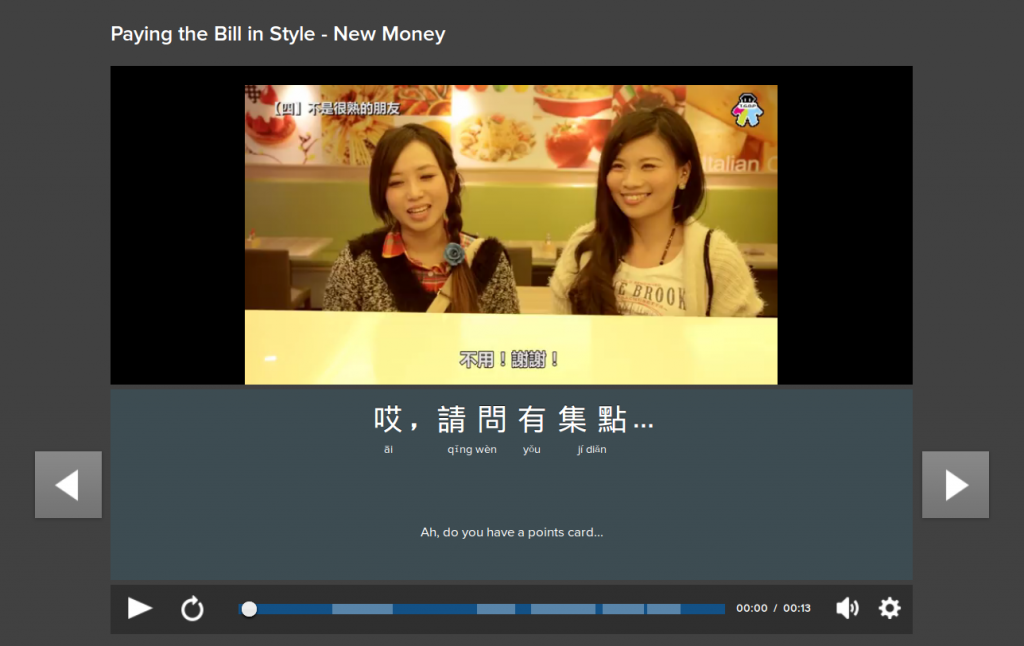
\includegraphics[width=1\textwidth]{./figs/fluentu-video.png}
    \caption{FluentU Platform Video Example}
    \label{fig:fluentu}
\end{figure}

LanguageReactor (formerly Language Learning with Netflix), as examined by~\citet{dizon2021}, is a free browser extension that allows users to overlay bilingual subtitles on Netflix and YouTube videos. It provides basic tools for vocabulary lookup and sentence by sentence playback. Unfortunately, it heavily relies on the availability of pre-existing subtitles and does not generate its own. This results in inconsistent subtitle quality. Figure \ref{fig:language-reactor-settings} shows the LanguageReactor settings page, which allows users to customize subtitle options. Figure~\ref{fig:language-reactor} shows an example of a video on the LanguageReactor platform, which includes bilingual subtitles and vocabulary tools.

\begin{figure}[H]
    \centering
    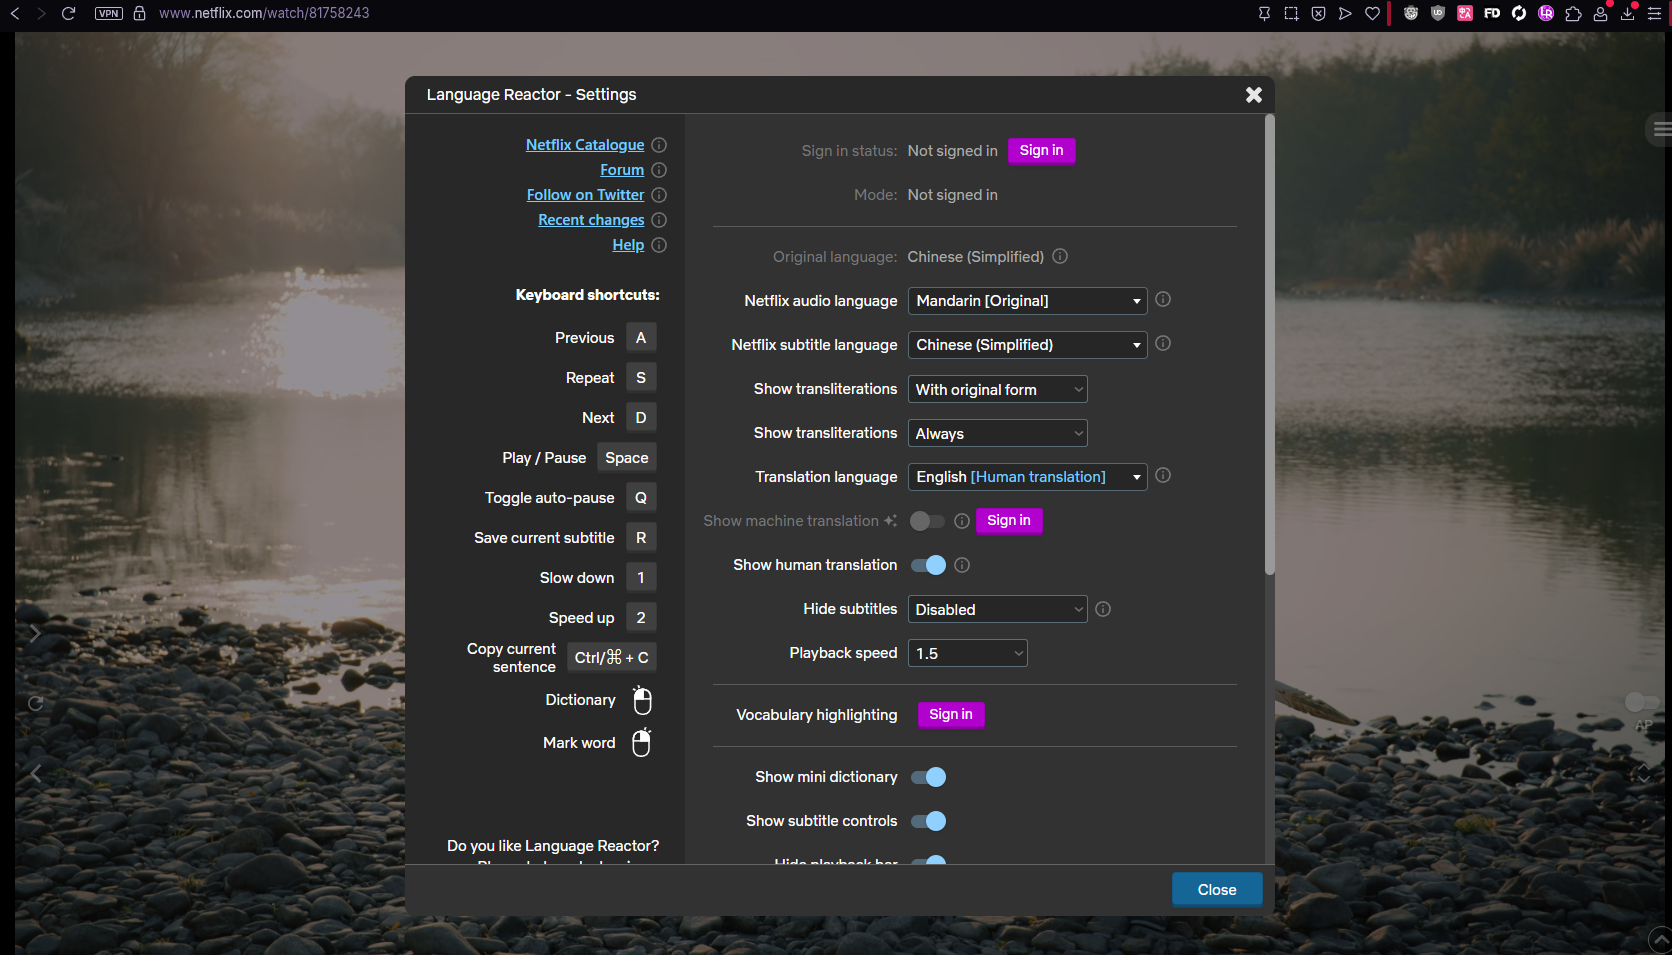
\includegraphics[width=1\textwidth]{./figs/lang_reactor-settings.png}
    \caption{LanguageReactor Settings Page From Netflix}
    \label{fig:language-reactor-settings}
\end{figure}

\begin{figure}[H]
    \centering
    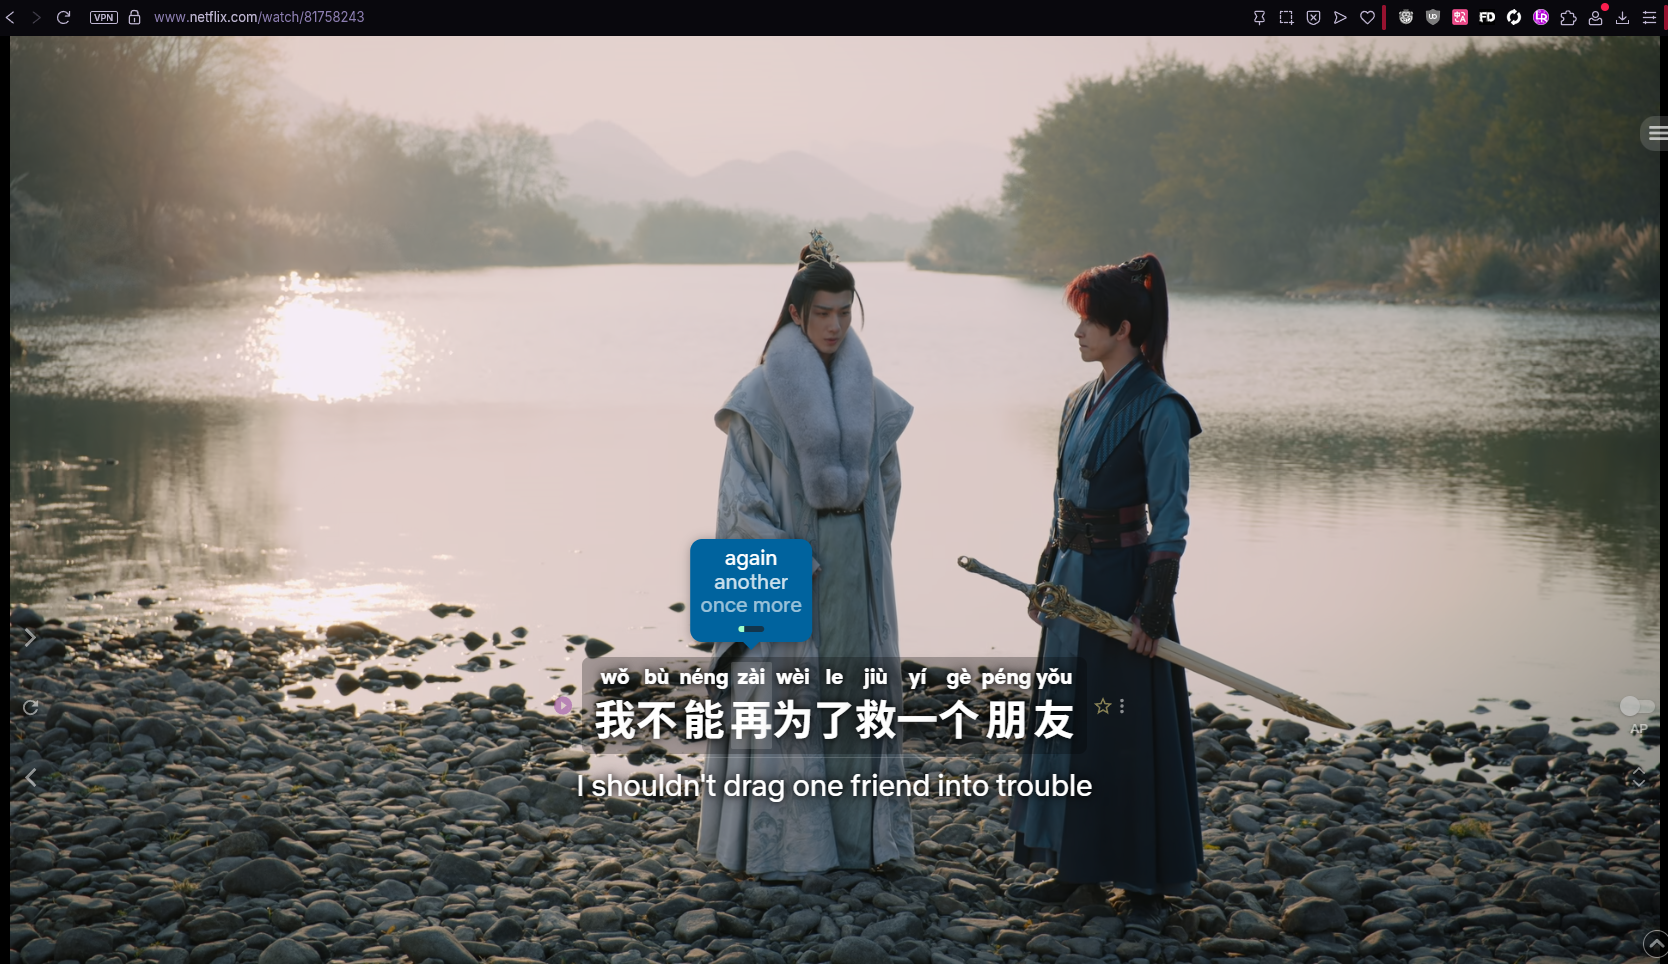
\includegraphics[width=1\textwidth]{./figs/lang_reactor.png}
    \caption{LanguageReactor Example From Netflix}
    \label{fig:language-reactor}
\end{figure}


Yabla is a subscription-based service that offers a curated video content library with interactive features. Research by~\citet{pujadas2024} demonstrated that Yabla's approach leads to better vocabulary retention compared to traditional video viewing methods. Although it provides a polished interface and well produced content, it is limited to a petite library of content that is lacking in scope and variety. However, the platform provides custom-created subtitles rather than relying entirely on third-party sources, which results in higher accuracy than LanguageReactor. Figure \ref{fig:yabla-browse} shows the Yabla platform's video browse page, which highlights its curated library of videos. Figure~\ref{fig:yabla} shows an example of a video on the Yabla platform, which includes interactive playback controls and vocabulary tools. the playback controls allow users to slow down or repeat specific segments, enhancing comprehension and retention.


\begin{figure}[H]
    \centering
    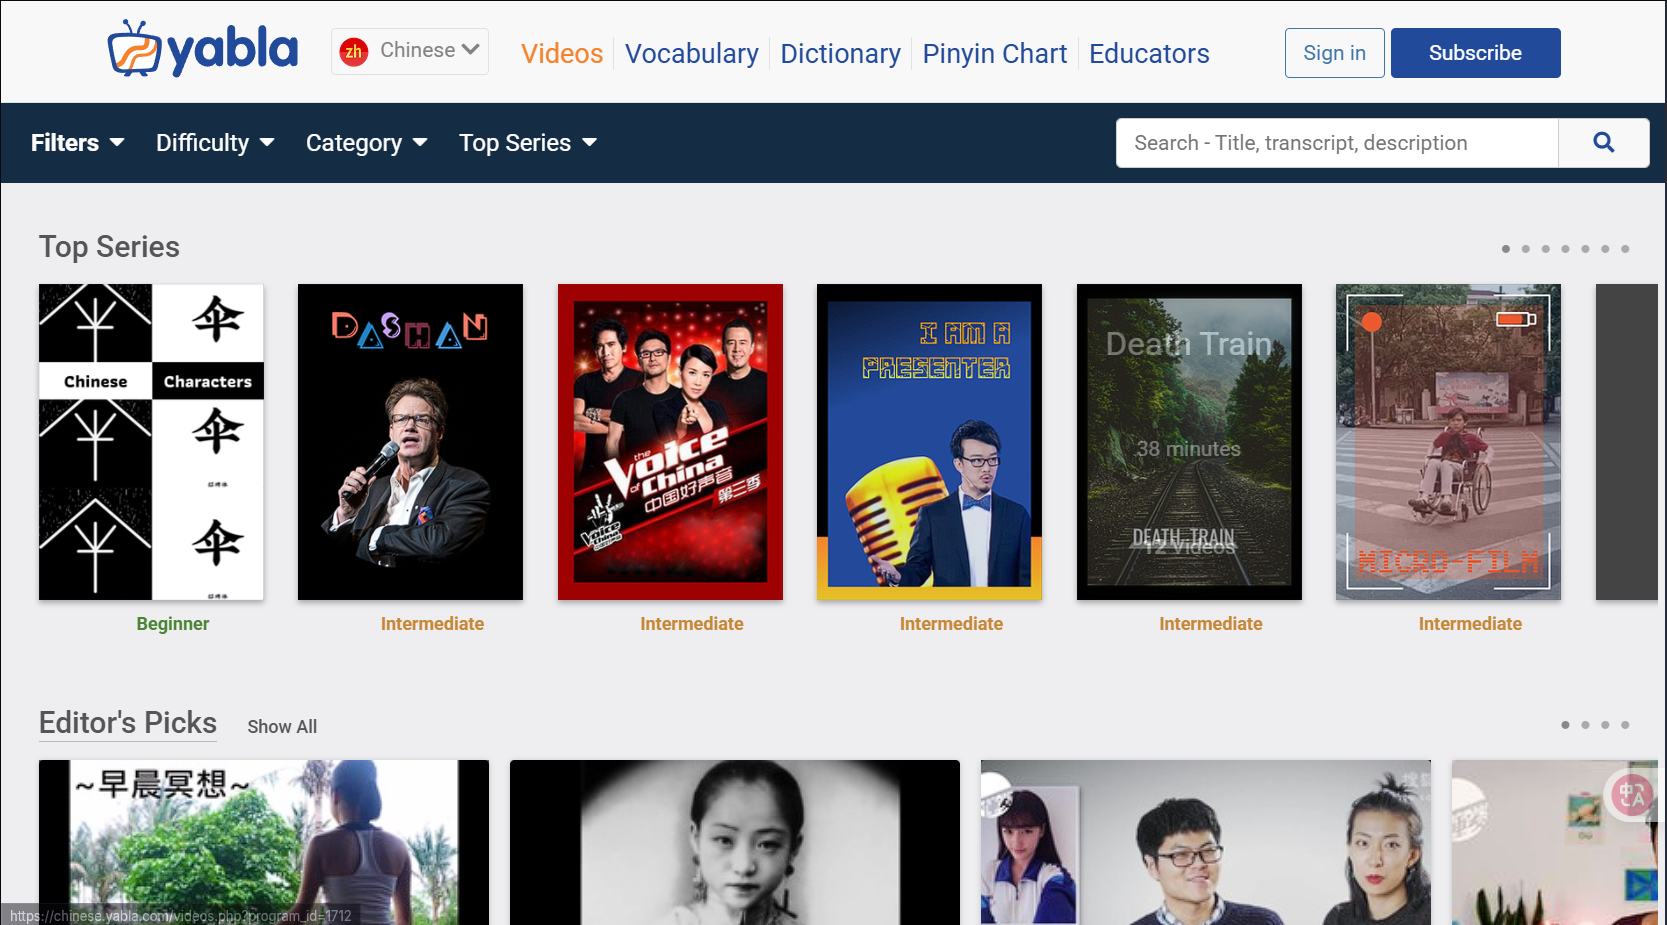
\includegraphics[width=1\textwidth]{./figs/yabla-video_browse.png}
    \caption{Yabla Platform Example}
    \label{fig:yabla-browse}
\end{figure}

\begin{figure}[H]
    \centering
    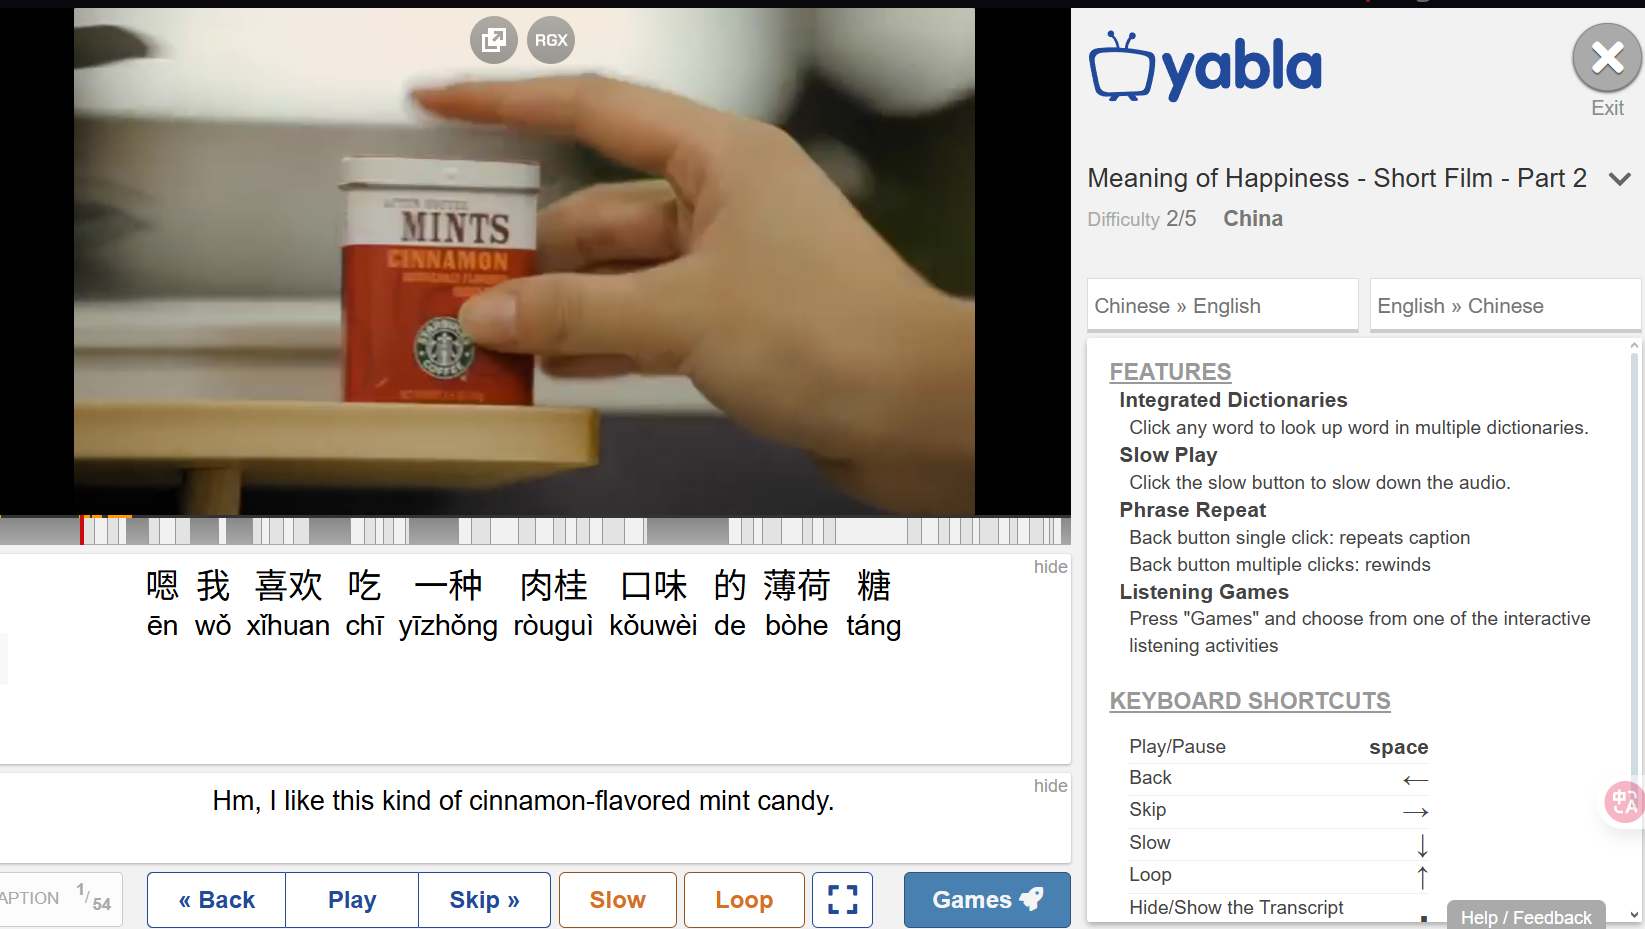
\includegraphics[width=1\textwidth]{./figs/yabla.png}
    \caption{Yabla Platform Video Example}
    \label{fig:yabla}
\end{figure}

The three systems already in place all make use of video content to learn a language, but they demonstrate distinct strategies to deal with the same core issue: the provision of engaging authentic video content supported by accurate language. The three platforms are all based on existing or handwritten subtitles{as shown in table~{\ref{tab:feature_comparison}}}. This leads to a content bottleneck that may have a negative impact on Mandarin learners because there is not enough content with subtitles. In particular when stacked against other languages in Europe such as French and German.

\begin{table}[h]
    \centering
    \caption{Language Learning Platform Feature Comparison}
    \scalebox{0.85}{
        \begin{tabular}{lllll}
            \toprule
            \textbf{Feature} & \textbf{Lang.Reactor} & \textbf{FluentU} & \textbf{Yabla}    & \textbf{{LexiFlow*}}      \\
            \midrule
            Content Source   & YT/Netflix subs       & Closed library   & Curated videos    & {Any Mandarin audio}      \\
            Pinyin Support   & Word-level            & Full             & Full              & {Full}                    \\
            Processing       & Existing subs         & Manual           & Manual            & {Auto segmentation}       \\
            Growth           & Subtitle-limited      & Slow manual      & Slow manual       & {Exponential User-driven} \\
            Efficiency       & High                  & Low              & Low               & {Medium}                  \\
            Cost             & Freemium              & Sub only         & Sub only          & {Freemium}                \\
            Personalization  & Basic vocab           & Adaptive quiz    & Playback controls & {Interest-based}          \\
            \bottomrule
        \end{tabular}
    }
    \label{tab:feature_comparison}

    \begin{flushleft}
        \small * Proposed solution
    \end{flushleft}
\end{table}

The automatic subtitle generation feature of LexiFlow enhances the existing platforms by removing the need for having pre-existing subtitles for any Mandarin audio/video content. Unlike other platforms that manage to upload and process content manually, this enables the content library to expand rapidly as more users upload and process their own content. LexiFlow operates under a freemium pricing model, providing people with free access to the basic features, and premium features such as flashcards and personalized quizzes for premium users. It also tailors learning to the user's interests, adds up what they've saved to their vocabulary list, and then suggests matching material and customizes study material – which makes learning more interesting and effective.


\section{Technologies for Video-Based Learning Platform}
\subsection{Voice Activity Detection and Sentence Segmentation}
VAD systems play crucial roles in several modern voice recognition frameworks, which require them to detect speech and non-speech segments frame-by-frame, and initiate the next actions, such as speech recognition and augmentation, or endpointing.~\citep{buddi2023,icassp-2019,chen2020,kumar2024}

On Mandarin,~\citet{pan2025} have shown that their system that splits the speech data into smaller segments based on the Silero-VAD model~\citep{sileroVAD} has better performance in boundary detection than a typical system. They discovered that they could get more accurate results by doing sentence-level segmentation rather than processing longer units. This figures into the segment-by-segment approach of LexiFlow.

\subsection{Automatic Speech Recognition for Mandarin}
Automatic Speech Recognition (ASR) was developed from basic systems that responded to a select few sounds to the modern systems that engage and interact with spoken languages. There has been a growing interest in ASR technology due to the desire to automate simple tasks that involve human-machine interaction~\citep{juang2005}.

OpenAI's Whisper~\citep{radford2023robust} is an automatic speech recognition (ASR) system trained on 680,000 hours of multilingual and multitask supervised data collected from the web.  The Whisper architecture is a simple end-to-end approach, implemented as an encoder-decoder Transformer. This architecture is used to transcribe and identify languages with high accuracy, even in noisy or demanding audio environments.

For educational applications,~\citet{sutomo2024} discovered that even with character error rates of 6--10\%, learners stated that ASR-generated transcripts were sufficient for understanding. This finding indicates that current ASR technology has reached the point of being usable in language learning applications such as LexiFlow.
\subsection{Neural Machine Translation}
Neural Machine Translation (NMT) has significantly improved the quality and dependability of automated translation services.  According to~\citet{hassan2018}, contemporary NMT systems have achieved human parity in Chinese-English translation for news domain content, marking a significant milestone for cross-linguistic applications.

~\citet{barrault2023seamless}  SeamlessM4T v2 is Meta's cutting-edge massively multilingual and multimodal machine translation model, intended to provide high-quality, real-time translation across speech and text in nearly 100 languages.  The v2 release features the UnitY2 architecture, which includes hierarchical character-to-unit upsampling and non-autoregressive decoding.

Importantly for LexiFlow,~\citet{gary2024} showed that even when translations had small faults, showing learners both the source text and machine translations increased understanding by when compared to source-only presentation. This result demonstrates that LexiFlow's strategy of offering translations in addition to the original Mandarin content works well.

\subsection{NoSQL Database Implementation}
NoSQL databases offer numerous benefits over traditional relational databases in the context of modern video-based learning platforms, such as flexibility, scalability, and performance. NoSQL systems do not require a fixed schema, which is ideal for storing content with varying types, like video metadata, user interactions, and dynamic learning analytics.

For unstructured and semi-structured data, NoSQL databases like document stores such as MongoDB are suitable to efficiently store and retrieve multimedia content, user profiles and session logs. This distributed architecture provides for high availability and horizontal scaling, essential for platforms with large numbers of users and a growing amount of content. Further, a key-value NoSQL database is good for read/write performance in real-time analytics, and a graph database can represent relations between concepts, users, and learning materials.

\section{Summary}
This literature review has established several key findings that inform LexiFlow's development. First, it was established that Krashen's Input Hypothesis and Multimedia Learning Theory provide strong theoretical foundations for LexiFlow's approach. After that, the Mandarin's symbolic writing system and its unique challenges was discussed. Furthermore, the current language learning applications and their limitations were carefully examined. Finally, This literature review was concluded by the recent advancements in Voice Activity Detection, Automatic Speech Recognition, and Neural Machine Translation and the discussion about the models which are planned to be used in the system.
% \begin{enumerate}[label= (\alph*)]
%     \item Krashen's Input Hypothesis and Multimedia Learning Theory provide strong theoretical foundations for LexiFlow's approach of making authentic content comprehensible through technological scaffolding.
%     \item Mandarin's logographic writing system creates unique challenges that require specialized technological solutions connecting spoken and written forms.
%     \item Current language learning applications demonstrate the value of authentic video content but suffer from critical limitations in content availability and flexibility.
%     \item Recent advances in Voice Activity Detection, Automatic Speech Recognition, and Neural Machine Translation have reached sufficient maturity to support educational applications with high accuracy.
%     \item Sentence-level processing approaches offer significant advantages in both computational efficiency and accuracy compared to whole-file processing.
%     \item Interest-driven learning consistently demonstrates superior engagement and outcomes compared to prescribed content approaches.
% \end{enumerate}
This review establishes both the need for and the feasibility of LexiFlow's approach to Mandarin language learning through efficient processing of authentic content. The next chapter will detail the methodological approach to implementing these insights in the LexiFlow system.

\chapter{SYSTEM DEVELOPMENT METHODOLOGY}
\section{Introduction}
This chapter outlines the methodology used in the development of LexiFlow to ensure the successful implementation of the system. The chapter opens with the explanation as to why the hybrid Agile model was selected and why it is appropriate to adopt elements from both Agile and traditional project management approaches to achieve a balance between flexibility and structure by keeping fixed development milestones in mind. Therefore, each phase of the adopted methodology will be elaborately discussed, which in effect will give an overall comprehensive framework that guides the development of the project from initial requirements gathering to the final stage of testing and deployment of the system.

The methodology section gives a more elaborate explanation as to how the
technologies chosen for our project would fit the features of the selected technologies within the Agile processes and aligns with the LexiFlow system itself. With this, the technology stack would support the functionality of the application.

\section{Methodology Choice and Justification}
LexiFlow's development was decided to follow the hybrid Agile model, as it allowed for flexibility to adapt to evolving requirements, while also providing structured milestones. This approach allows for iterative development, allowing for ongoing feedback and refinement throughout the project lifecycle. Agile is well suited to software projects where the needs of the users can change, because it focuses on collaboration, customer involvement and adaptation to change.

As reported by~\citet{scrum} implementing Scrum might help to enhance software product quality, communication and cooperation.  Waterfall's benefits are that the phases are arranged in order to help new developers get a complete understanding of the `big picture`of software project management, throughout the Software Development Life Cycle.  This also helps in having much deeper understanding of the requirements, code logic and software testing.

Throughout the development process, the following principles of Agile will be used: regular sprints, user stories, and continuous integration. The project will also be managed using traditional project management practices, including detailed planning and documentation, to ensure that all aspects of the system are well covered, as shown in figure {\ref{fig:methodology_overview}}.

\begin{figure}[ht]
    \centering
    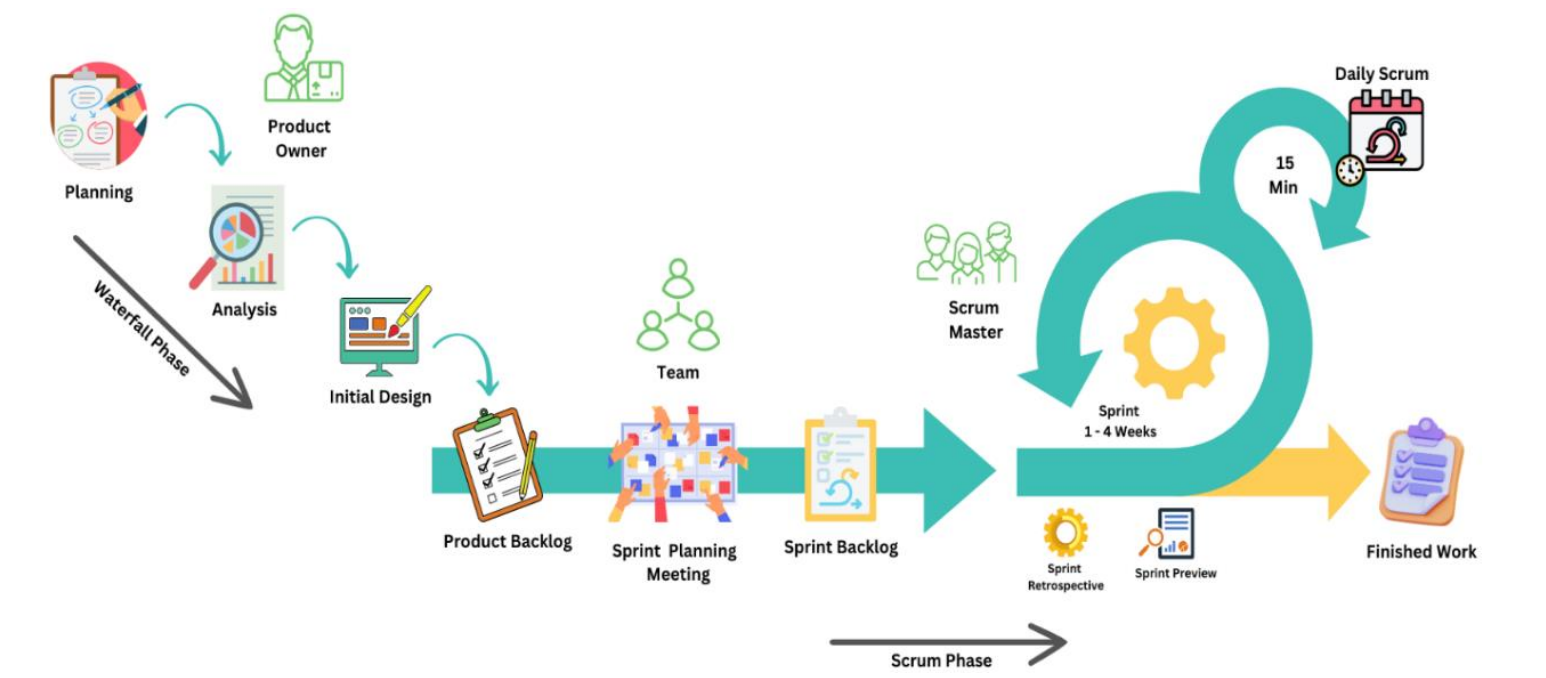
\includegraphics[width=1\textwidth]{./figs/scrum2.png}
    \caption{Hybrid-Scrum Methodology Overview~\citep{scrum2}}
    \smallskip
    \label{fig:methodology_overview}
\end{figure}

\section{Methodology Phases}

LexiFlow will be developed using a hybrid approach:
\begin{enumerate}[label= (\alph*)]
    \item \textbf{Planning (Waterfall):} This phase prepares the overall project. It involves a preliminary project scoping, time estimation, stakeholder identification and resource assignment. The planning process follows a Waterfall method, with all the planning steps of the roadmap being planned in advance to give a clear direction of the project at the start.

    \item \textbf{Analysis (Waterfall):} This is the part of the project where all the project requirements will be studied thoroughly and recorded in a waterfall method of development. The process involves all stakeholders, language learners and lecturers, in a detailed interview/survey to try to define all functional and non-functional requirements as thoroughly as possible.

    \item \textbf{Initial Design (Waterfall):} After requirements are established, project will go directly into design phase using the Waterfall method. This step creates a high level design of the system as a whole, and this sets out how each component interfaces with the other components of the system. This can be extremely appropriate for the user requirements, so that each part of the system is well defined and ready to go into development.

    \item \textbf{Actual Sprints (Agile):} The development will take place in six sprints (Agile):

          \begin{enumerate}[label= (\roman*)]
              \item \textit{Sprint 1 ~ Prototype Sprint:} Sprint 1 involves creating an initial prototype with basic functions to test the assumptions of the early design, to collect feedback and to verify the performance of the selected models.

              \item \textit{Sprint 2 ~ User Module:} This sprint is dedicated to implementing user registration, login and profile management. It enables both students and lecturers to create and manage their accounts and learning preferences.

              \item \textit{Sprint 3 ~ Content Processing Module:} During this sprint, the functionality to upload local media and submit the link to the YouTube website is implemented. The content will be processed by the system and produce synchronized subtitles in Mandarin, pinyin, and English translation.

              \item \textit{Sprint 4 ~ Interactive Learning Module:} This sprint will implement the interactive learing module to implement the features such as word search, bookmarking segenents and reporting incorrect translations.

              \item \textit{Sprint 5 ~ Assessment Module:} This sprint will contain the fucntional testing and user acceptance testing. this will involve testing with users and stakeholders.

              \item \textit{Sprint 6 ~ Deployment Sprint:} This sprint will involve deploying and tesing the deployment on live servers.
          \end{enumerate}

    \item \textbf{Burn Down Chart (Agile):} A burn down chart is also provided for the Agile method to show what tasks remain to be completed over time during each sprint. This visual tool can be used by the team to track progress on a day-to-day basis, to identify any bottlenecks quickly, and to make sure the sprint is progressing to the desired direction and toward the desired outcome. It is also a good reference point for the Sprint Review.

    \item \textbf{Sprint Review (Agile):} During Sprint Review, features added to the application are shown to the stakeholders at the end of each sprint. The input from their feedback is captured and incorporated into the next set of sprint goals, thus keeping them in line with what users expect.

    \item \textbf{Sprint Retrospective (Agile):} After every Sprint Review, the team has Sprint Retrospective, which is an agile process that helps the team evaluate what they did well, what they did not do well, and what they can do better in the next Sprint. This helps to foster ongoing improvements and teamwork.

    \item \textbf{Maintenance (Agile):} After deployment, the system will go into the maintenance phase, which is also called "Agile". The addition of bugs fixes, user feedback and new features will be provided in incremental releases using Agile practices, and will keep the product strong and user-focused over time.
\end{enumerate}

Gannt chart in Figure~\ref{fig:jira} shows the timeline of the FYP 1 and the prototype sprint while Figure~\ref{fig:jira2} shows the timeline of FYP 2. The Gannt chart is created using Jira, which is a project management tool that helps to track the progress of the project and manage the tasks effectively.


\begin{figure}[H]
    \centering
    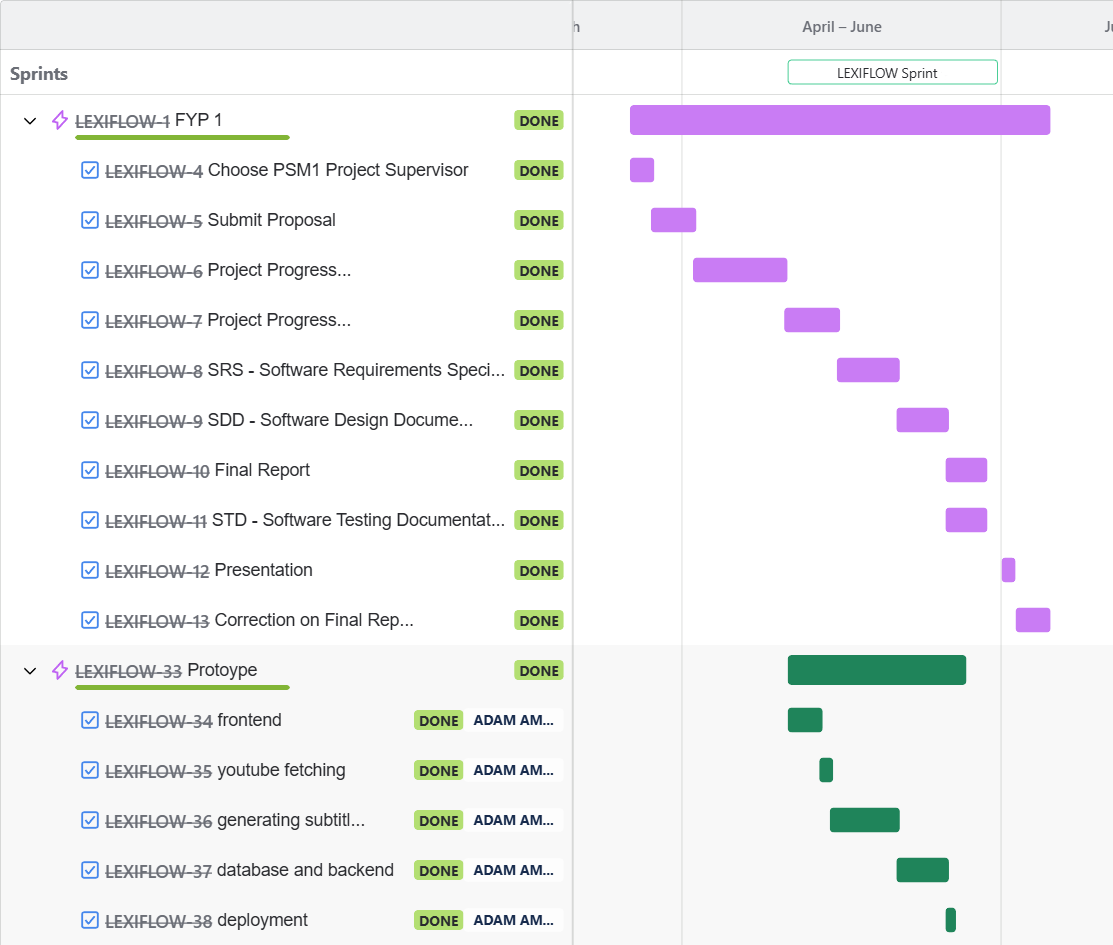
\includegraphics[width=0.75\textwidth]{./figs/fyp1_gantt.png}
    \caption{Gantt Chart FYP1}\label{fig:jira}
\end{figure}

\begin{figure}[H]
    \centering
    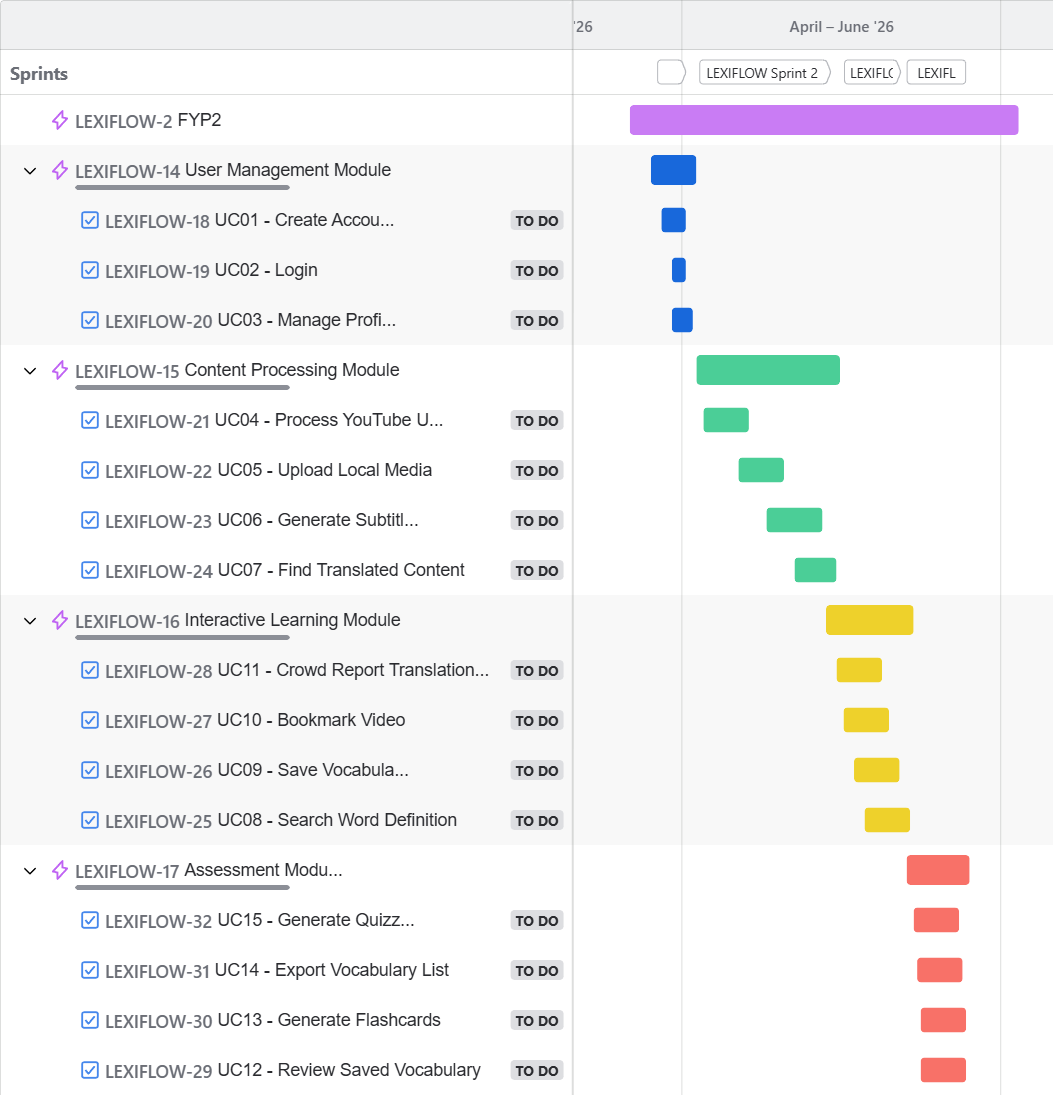
\includegraphics[width=0.75\textwidth]{./figs/fyp2_gantt.png}
    \caption{Gantt Chart FYP2}\label{fig:jira2}
\end{figure}

The first sprint is the prototype sprint, which is already completed. The burn down chart is shown in Figure~\ref{fig:burndown}. The burn down chart shows the progress of the project and the remaining tasks to be completed. Also, the sprint review with the stakeholders is completed. The feedback from the stakeholder is shown in Appendix~\ref{app:feedback-on-prototype}.

\begin{figure}[H]
    \centering
    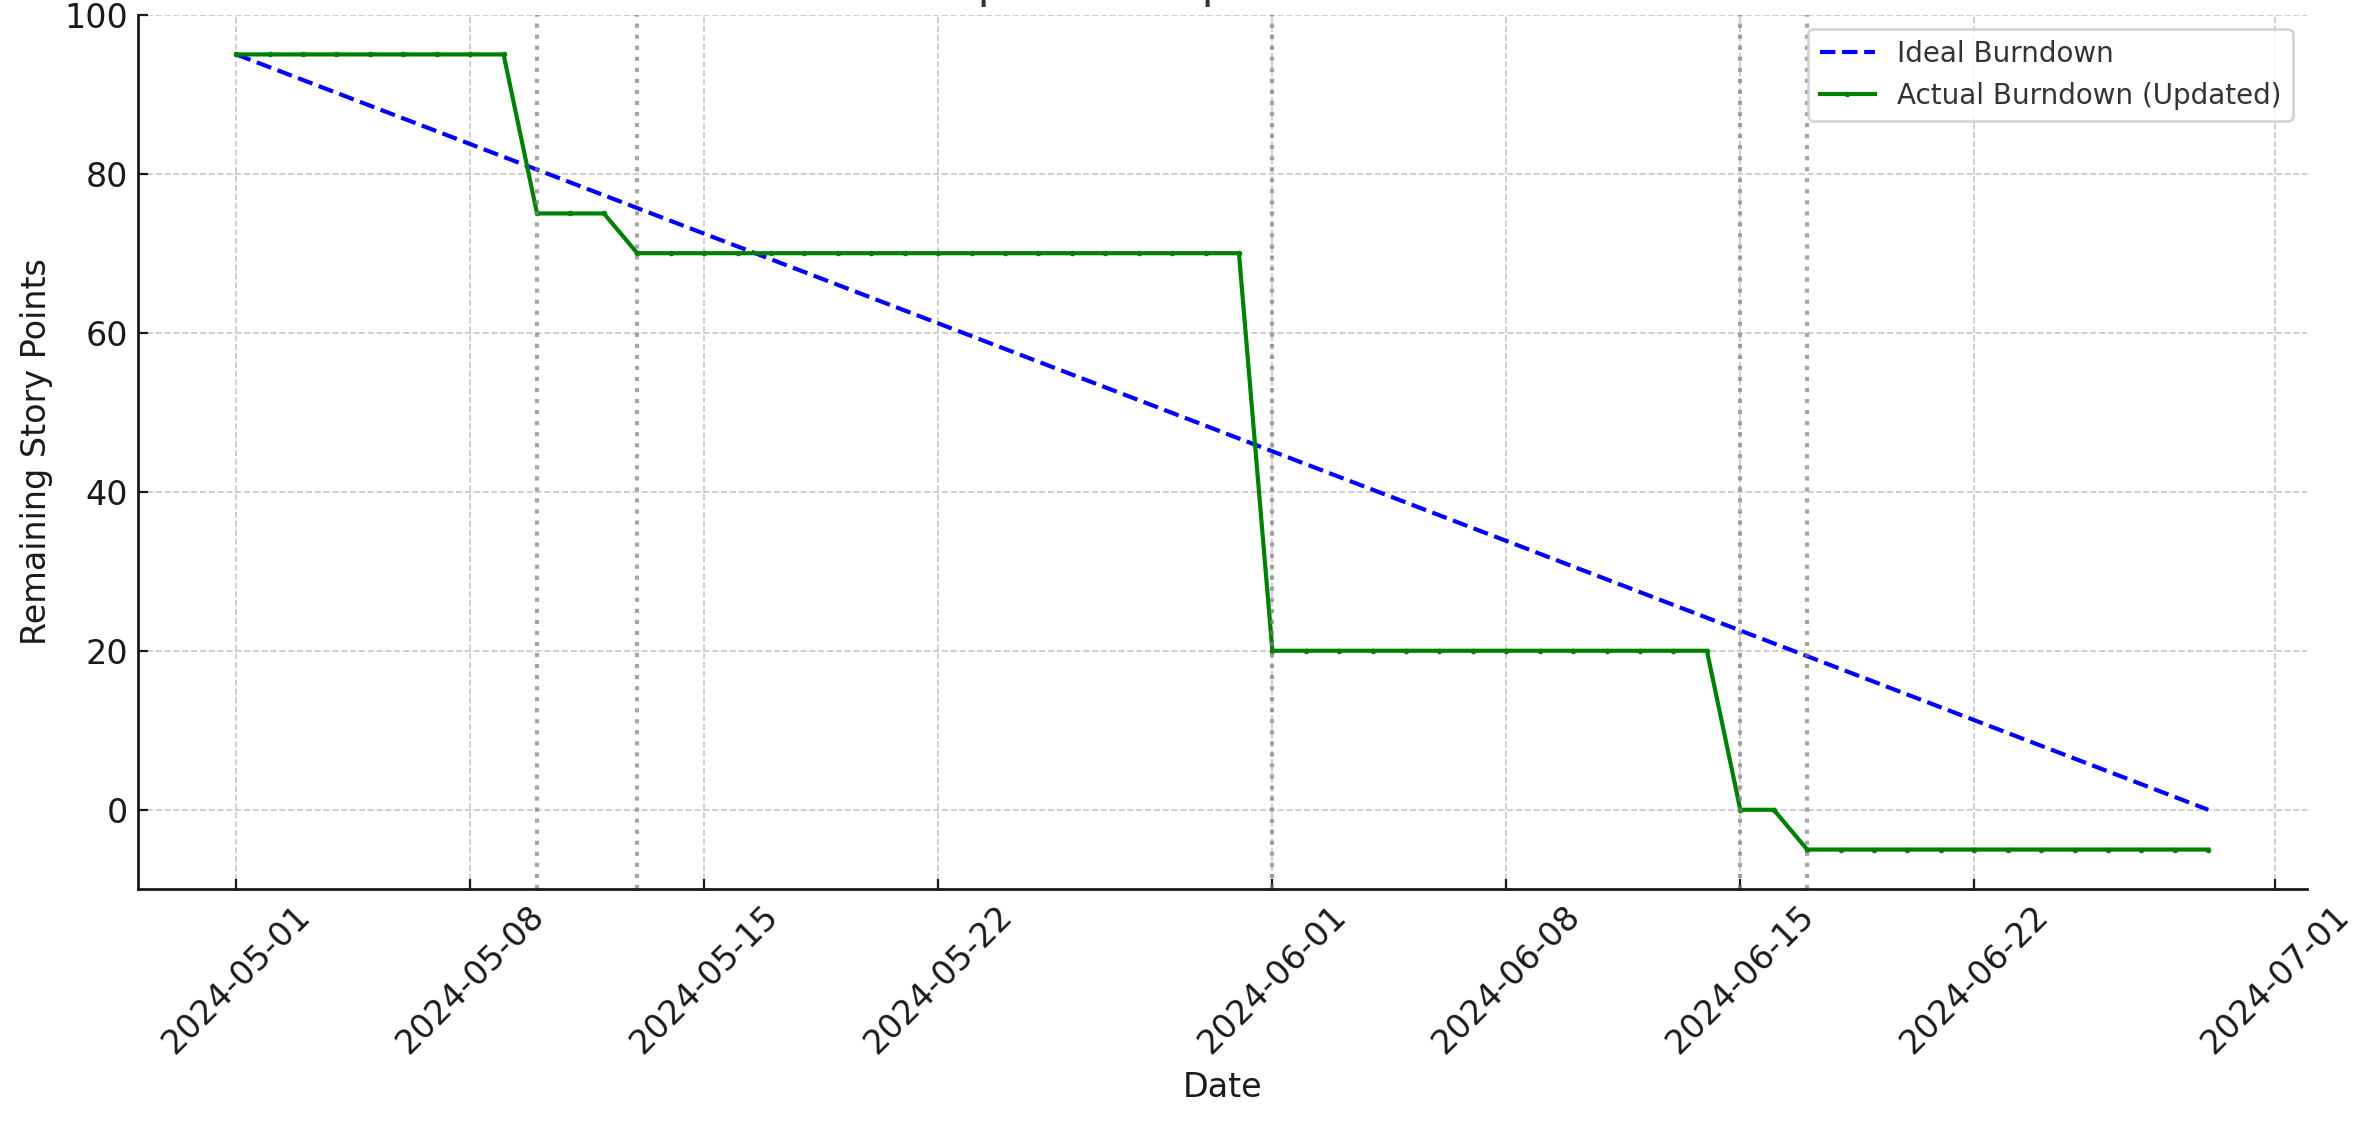
\includegraphics[width=0.8\textwidth]{./figs/burndown.png}
    \caption{Burn Down Chart for Sprint 1 (Prototype)}\label{fig:burndown}
\end{figure}

\section{Technology Stack}
This section describes the technologies used in the development of the LexiFlow system.  The following technologies were identified for their capacity to meet the project's requirements:

\begin{enumerate}[label= (\alph*)]
    \item \textbf{Vue.js:} A JavaScript framework for creating user interfaces.  Vue.js was chosen for its reactive and compiler-optimized rendering system. It will be used to create the frontend of the web application.
    \item \textbf{Node.js:} a JavaScript runtime based on Chrome's V8 engine. It was chosen for its non-blocking and event-driven architecture. That makes it suitable for developing scalable network applications. It will be used for server-side logic and user request management. Furthermore, It will act as the control center of our backend services, handling requests from the frontend and coordinating with the database and python microservices.
    \item \textbf{MongoDB:} MongoDB is a document database designed to help developers build modern applications faster. It stores data in flexible, JSON-like documents, making it easy to model data the same way your application code uses it. The flexible schema lets you evolve your data model without downtime, iterate quickly, and easily handle non-uniform data.
    \item \textbf{FastApi:} A modern, high-performance web framework that aims to simplify the development of APIs with Python, using standard Python type hints. FastAPI was chosen because of its ease of use and automatic documentation creation. It will be used by the backend services to convert the python scripts into RESTful APIs, allowing our Node.js server to communicate with the services that handle audio processing, transcription, and translation.
    \item \textbf{SileroVAD:} Silero VAD works effectively with audios from a variety of domains with a range of background noise and quality levels. It was trained on a massive dataset that included over 6000 languages. It was chosen for its high accuracy and ease of use. It will be used to detect speech segments and segment them into sentence-level chunks.
    \item \textbf{Whisper:} a powerful automated speech recognition system that was trained on a diverse dataset of multilingual speech data. It was chosen for its high accuracy and ability to handle various languages and accents. It will be used to transcribe the audio content into text, providing the foundation for further processing.
    \item \textbf{SeamlessM4Tv2:} The SeamlessM4T-v2 model was proposed in~\citep{communication2023seamlessmultilingualexpressivestreaming} by the Seamless Communication team from Meta AI. SeamlessM4T-v2 is a collection of models designed to provide high quality translation, allowing people from different linguistic communities to communicate effortlessly through speech and text. It is an improvement on the previous version.
    \item \textbf{PyPinyin:} pypinyin is a Chinese Pinyin conversion tool that supports multiple lexicons, multiple output formats, and custom word group Pinyin libraries or single-character Pinyin libraries.

\end{enumerate}

LexiFlow's development process employs automated workflows, ensuring smooth updates. First, developers commit changes to the code to version control in Git, as is illustrated in Figure~\ref{fig:ci_cd}. The code is then automatically built and tested on GitHub Actions. Lastly, the working application is packaged in Docker for deployment via Nginx. This automatic pipeline enables the identification of mistakes at an early stage and stable releases.

It is obvious from the figure how these steps link with our planning and monitoring which ensure development is efficient and reliable. This helps us to follow our hybrid Agile approach, allowing for regular updates without compromising the stability of the system.

\begin{figure}[H]
    \centering
    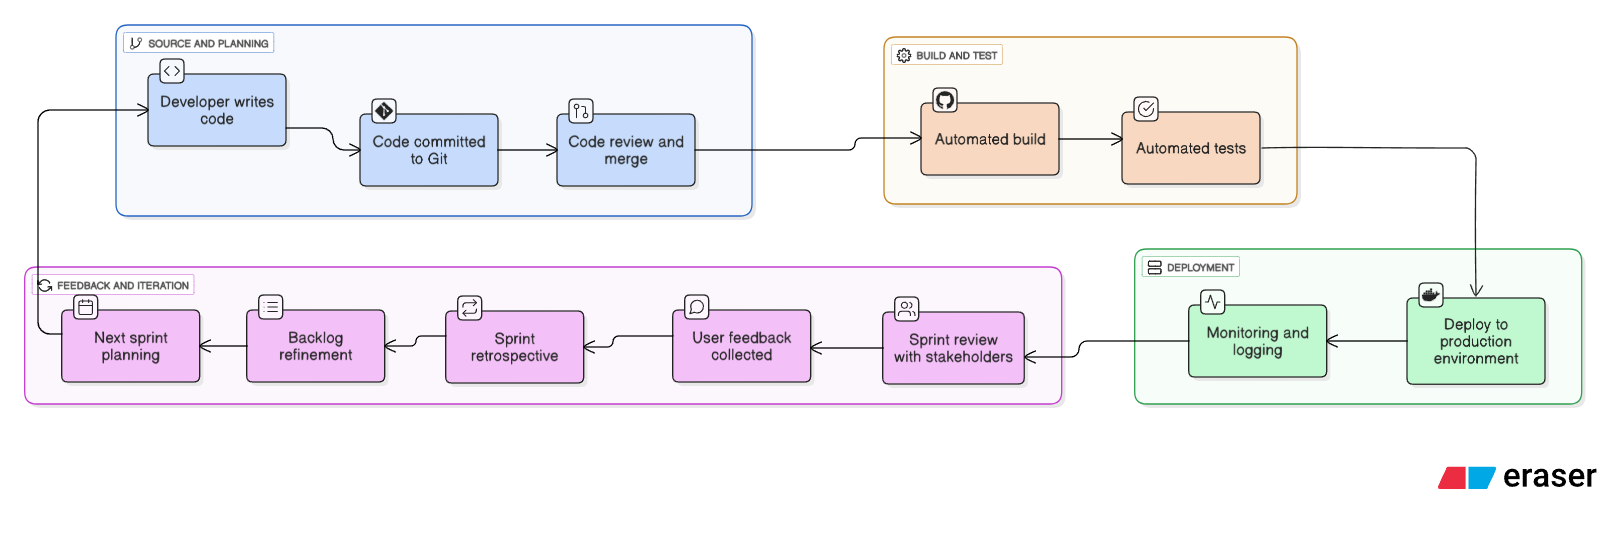
\includegraphics[width=1\textwidth]{./figs/ci_cd.png}
    \caption{CI/CD Pipeline for LexiFlow}\label{fig:ci_cd}
\end{figure}

\section{System Requirement Analysis}
This section gives details of system requirements that includes all hardware, software and other requirements. They will be helpful for fulfilling the functional and performance requirements, and can ensure successful development and operation of the above system.

\subsection{Hardware Requirements}
These are the hardware requirements for the optimal deployment and user experience of the LexiFlow system:
\begin{enumerate}[label= (\alph*)]
    \item \textbf{Server:} A dedicated server equipped with at least 16 GB of RAM, 8 CPU cores, and 500 GB of SSD storage for the back-end processing, database management and API requests. In addition, for effectively processing audio material, at least 8GB of graphics memory is necessary, particularly when dealing with tasks such as automatic speech recognition and machine translation.
    \item \textbf{Development Machines:}  To run development environments, testing frameworks, and local databases, development machines should have a minimum of 8 GB of RAM, enough storage (at least 256 GB SSD), and a modern multi-core processor.
    \item \textbf{Client Devices:} Users should be able to use devices that have at least 4 GB of RAM, and a modern browser (Chrome, Firefox, Safari) to interact with the LexiFlow web application.
\end{enumerate}

\subsection{Software Requirements}
The LexiFlow system will require the following software components:
\begin{enumerate}[label= (\alph*)]
    \item \textbf{Operating System:} An operating system that is Linux-based (e.g., Ubuntu 22.04 or later) for the server environment to ensure stability and performance.
    \item \textbf{Web Server:} Nginx as the web server to handle HTTP requests and serve the LexiFlow web application.
    \item \textbf{Database:} MongoDB for storing user data, audio/video metadata, and processed subtitles.
    \item \textbf{Version Control:} Git to manage code changes and manage versions.
    \item \textbf{Network Protocols:} SSH to securely access the server remotly.
    \item \textbf{IDE:} Visual Studio Code, providing features like code completion, debugging, and version control integration.
    \item \textbf{Visual Design Tools:} Enterprise Architect to design the system architecture and UML diagrams. Figma to create user interface mockups.
\end{enumerate}



\section{Chapter Summary}
This chapter guides through the approach that was taken by LexiFlow with special emphasis on the hybrid Agile framework that combines both iterative development with structured phases. That way, the project could be agile enough to adapt to changing needs but still possess milestone checks. The technology stack has also been discussed in detail with the rationale of each decision. Lastly, the hardware and software requirements are also outlined, which sets the stage of a successful implementation in the subsequent phases.

\chapter{REQUIREMENT ANALYSIS AND DESIGN}
\section{Introduction}
This chapter provides an overview of the phases of requirement analysis and design stages for the LexiFlow project, which shows the way for the development of a systematically organised language learning system designed for the UTM community. The chapter adheres to a systematic way of identification and analysis of specific requirements of various stakeholders through structured interactions like surveys and interviews.

After the detailed requirement analysis is conducted, the chapter then proceeds to design the system. This involves looking at the design of a system architecture supporting seamless interactions between the various components of LexiFlow. This involves designing the modular structure of the system and how those different modules communicate with each other, ensuring that the architecture affects the set-out goals of the project.

\section{Requirements Gathering and Analysis}

The requirements for the LexiFlow project were analysed meticulously through an interview session with the stakeholders from UTM Language Academy. This was an essential process in detailing the limitations of the existing system and what specific needs the stakeholders have for the proposed LexiFlow platform. Their information indicated the dire necessity for an automated solution that effectively processes authentic Mandarin content, providing learners with synchronized audio, pinyin, and English translations.

A greater emphasis was placed during the analysis on the following key functionalities identified as necessary for improving the overall effectiveness of the system: features for user evaluation, such as flashcards, quizzes and others as well as themed playlist features to ensure learning is more organized and structured. These kinds of features are expected to improve the learning process.  Figure~\ref{fig:use_case} below details the use case diagram of LexiFlow implementing the features stated previously.

\begin{figure}[h!]
    \centering
    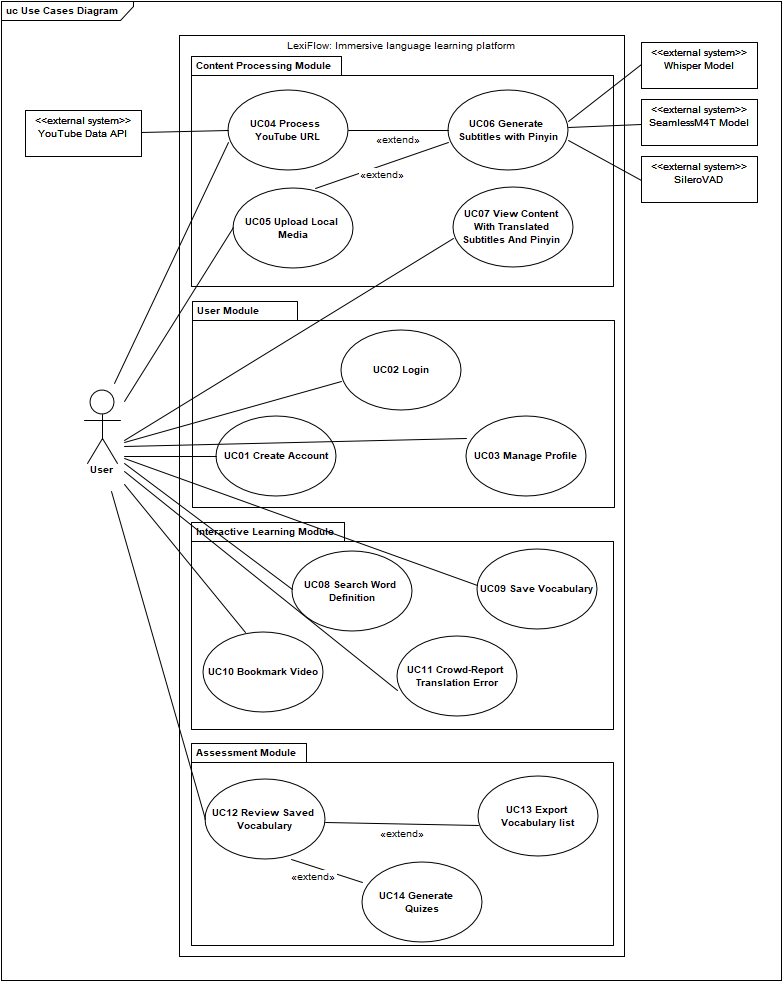
\includegraphics[width=0.8\textwidth]{./figs/use_cases.png}
    \caption{Use Case Diagram of LexiFlow}\label{fig:use_case}
\end{figure}

The requirement analysis phase ended with a proper understanding of the system specifications and functionalities. Such requirements are aimed at guiding the subsequent phases in the design and development of a system. Although the project development is done purposely to align with the needs and expectations of the UTM community, LexiFlow also looks toward overcoming the deficiencies of the current system and innovative features enhancing user experience and safety. Such an approach is likely to result in the development of a final product well tailored to
satisfy specific demands of the UTM community.

\subsection{Functional Requirements}
The functional requirements of LexiFlow are derived from the use case diagram (Figure~\ref{fig:use_case}) and are shown in Table~\ref{tab:functional_requirements}.
\begin{longtable}{>{\centering\arraybackslash}m{1.2cm} >{\centering\arraybackslash}m{3cm} >{\arraybackslash}m{8cm}}
    \caption{Functional Requirements of LexiFlow System}\label{tab:functional_requirements}                                     \\
    \toprule
    \textbf{ID} & \textbf{Name}                  & \textbf{Description}                                                         \\
    \midrule
    \endfirsthead
    \multicolumn{3}{l}{\textit{(Continued from previous page)}}                                                                 \\
    \toprule
    \textbf{ID} & \textbf{Name}                  & \textbf{Description}                                                         \\
    \midrule
    \endhead
    \midrule
    \multicolumn{3}{r}{\textit{(Continued on next page)}}                                                                       \\
    \endfoot
    \bottomrule
    \endlastfoot
    UC01        & Create Account                 & Allows new users to register and create an account in the system.            \\
    UC02        & Login                          & Enables registered users to authenticate and access the system.              \\
    UC03        & Manage Profile                 & Allows users to view and update their personal information and preferences.  \\
    UC04        & Process YouTube URL            & Handles the processing of YouTube video URLs for content extraction.         \\
    UC05        & Upload Local Media             & Enables users to upload media files from their local device for processing.  \\
    UC06        & Generate Subtitles             & Automatically creates subtitles for processed video content.                 \\
    UC07        & Find Translated Content        & Provides functionality to locate translated versions of content.             \\
    UC08        & Search Word Definition         & Allows users to search for definitions of words within the learning module.  \\
    UC09        & Save Vocabulary                & Enables users to save new vocabulary words for later review.                 \\
    UC10        & Bookmark Video                 & Allows users to bookmark specific video segments for future reference.       \\
    UC11        & Crowd-Report Translation Error & Provides a mechanism for users to collaboratively report translation errors. \\
    UC12        & Review Saved Vocabulary        & Enables users to review and practice vocabulary they have previously saved.  \\
    UC13        & Export Vocabulary list         & Allows users to export their vocabulary lists for use outside the system.    \\
    UC14        & Generate Quizes                & Automatically creates quizes from saved vocabulary for study purposes.       \\
\end{longtable}

As an example, the use case for processing YouTube URLs (UC04), shown in Table~\ref{tab:use_case_uc04}, involves key actors such as the user and the YouTube Data API. The system extracts video content by validating the URL, retrieving metadata, and checking the duration of the video.

All use cases, including detailed descriptions of the normal flow, alternative flows (such as handling invalid duration or restricted content), and exception flows, are fully documented in the Software Requirements Specification (SRS). The complete use case specifications can be found in Appendix~\ref{app:srs}.

\begin{longtable}{|>{\columncolor[HTML]{D9D9D9}}l|p{10cm}|}
    \caption{Use Case Description for UC04 \textless{}Process YouTube URL\textgreater{}}\label{tab:use_case_uc04}
    {}                                                                                                                                                                                                        \\
    \hline
    \textbf{Use Case ID}           & UC04                                                                                                                                                                     \\
    \hline
    \textbf{Use Case Name}         & Process YouTube URL                                                                                                                                                      \\
    \hline
    \textbf{Description}           & This use case allows an authenticated user to submit a YouTube video URL for automated transcription, translation, and synchronized subtitle generation within LexiFlow. \\
    \hline
    \textbf{Actor(s)}              & User, YouTube Data API                                                                                                                                                   \\
    \hline
    \textbf{Pre-conditions}        &
    1. The user is successfully logged into their LexiFlow account.                                                                                                                                           \\
                                   & 2. The LexiFlow system has internet access to reach YouTube.                                                                                                             \\
                                   & 3. System has active connection to YouTube Data API                                                                                                                      \\
    \hline
    \textbf{Normal Flow (NF)}      &
    1. User navigates to "Upload/Process Content" section                                                                                                                                                     \\
                                   & 2. User selects option to process YouTube URL                                                                                                                            \\
                                   & 3. User inputs valid YouTube video URL                                                                                                                                   \\
                                   & 4. User submits URL for processing                                                                                                                                       \\
                                   & 5. System validates URL and fetches video stream                                                                                                                         \\
                                   & 6. System initiates content processing pipeline                                                                                                                          \\
                                   & 7. System notifies user that processing has started                                                                                                                      \\
    \hline
    \textbf{Alternative Flow (AF)} &
    AF1: Invalid YouTube URL                                                                                                                                                                                  \\
                                   & \quad 1. If URL is invalid or video not found:                                                                                                                           \\
                                   & \quad \quad 1.1 System displays "Invalid YouTube URL" error                                                                                                              \\
                                   & \quad \quad 1.2 Prompts user to enter correct URL                                                                                                                        \\
                                   & AF2: Restricted/Private Video                                                                                                                                            \\
                                   & \quad 1. If video is regionally restricted or private:                                                                                                                   \\
                                   & \quad \quad 1.1 System displays access restriction error                                                                                                                 \\
                                   & \quad \quad 1.2 Use case terminates unsuccessfully                                                                                                                       \\
    \hline
    \textbf{Exception Flow (EF)}   &
    EF1: Processing Pipeline Failure                                                                                                                                                                          \\
                                   & \quad 1. If content processing encounters critical error:                                                                                                                \\
                                   & \quad \quad 1.1 System logs detailed error                                                                                                                               \\
                                   & \quad \quad 1.2 Displays generic failure message                                                                                                                         \\
                                   & \quad \quad 1.3 Use case terminates unsuccessfully                                                                                                                       \\
                                   & EF2: Network Error During Fetch                                                                                                                                          \\
                                   & \quad 1. If network issue prevents video fetching:                                                                                                                       \\
                                   & \quad \quad 1.1 System displays network error message                                                                                                                    \\
                                   & \quad \quad 1.2 Prompts user to check connection                                                                                                                         \\
                                   & \quad \quad 1.3 Use case terminates unsuccessfully                                                                                                                       \\
    \hline
    \textbf{Post-conditions}       &
    1. YouTube video content is successfully extracted                                                                                                                                                        \\
                                   & 2. Content processing pipeline is initiated                                                                                                                              \\
                                   & 3. User receives processing status notification                                                                                                                          \\
    \hline
    \textbf{Special Requirements}  &
    1. System has internet access to reach YouTube                                                                                                                                                            \\
                                   & 2. YouTube video processing capabilities                                                                                                                                 \\
    \hline
\end{longtable}

\subsection{Non-Functional Requirements}
Non-functional requirements specify quality attributes, system performance and constraints that LexiFlow must satisfy. These requirements are crucial for ensuring the system's reliability, usability, and maintainability. A list of non-functional requirements is presented in Table~\ref{tab:non_functional_requirements}.

\begin{longtable}{>{\centering\arraybackslash}m{1.2cm} >{\centering\arraybackslash}m{3cm} >{\arraybackslash}m{8cm}}
    \caption{Non-Functional Requirements}
    \label{tab:non_functional_requirements}                                                                                                 \\
    \hline
    \textbf{ID} & \textbf{Type} & \textbf{Description}                                                                                      \\
    \hline
    \endfirsthead
    \multicolumn{3}{l}{\textit{(Continued from previous page)}}                                                                             \\
    \hline
    \textbf{ID} & \textbf{Type} & \textbf{Description}                                                                                      \\
    \hline
    \endhead
    \hline
    \multicolumn{3}{r}{\textit{(Continued on next page)}}                                                                                   \\
    \endfoot
    \hline
    \endlastfoot
    NFR-001     & Performance   & The system shall process and validate YouTube URLs within 3 seconds to ensure responsive user experience. \\
    \hline

    NFR-002     & Localization  & The system shall support display text in at least two languages: English and Mandarin.                    \\
    \hline

    NFR-003     & Backup        & System data shall be backed up automatically every 24 hours and stored securely                           \\
\end{longtable}

\section{Architectural Design}

The Pipe and filter architectural pattern is a method of structuring the processing as a series of discrete components, called filters, linked together by pipes. Every filter takes the data, applies a particular transformation or processing and outputs the transformed data to the next filter through a pipe. Scalability, maintainability, and reusability are improved due to the modular approach, with filters being developed, tested, and replaced separately. The clear separation of concerns also makes system extensions and debugging easier in the future.

In the audio processing pipeline of LexiFlow, each filter can perform a unique function like voice activity detection, speech recognition, translation, and pinyin generation, making the Pipe and Filter pattern suitable. The versatility of this modularity makes it simple to add new processing steps or to substitute out old steps without changing the system architecture.


The architecture of the LexiFlow system is composed of various components as depicted in Figure~\ref{fig:pipe_and_filter}:


\begin{enumerate}[label= (\alph*)]
    \item \textbf{User Interface (UI):} The user interface (UI) created using Vue.js, which is an interactive application for users to upload media, view subtitles, and manage vocabulary. Has been viewed as the source of data in the Pipe and Filter architecture.
    \item \textbf{Backend Services:} The back end services are the implementation on top of Node.js and FastAPI, which process audio and video content, and are regarded as pipes in the Pipe and Filter architecture.
    \item \textbf{Audio Processing Pipeline:} These are a sequence of filters that process the voice signals to detect any voice activity (SileroVAD), automatic speech recognition (Whisper), translation (SeamlessM4Tv2), and generation of pinyin (pinyin).
    \item \textbf{Database:} User profiles, processed content metadata, subtitles and vocabulary lists are stored in MongoDB. In the Pipe and Filter design, it is viewed as the place to "sink" data.
\end{enumerate}

\begin{figure}[H]
    \centering
    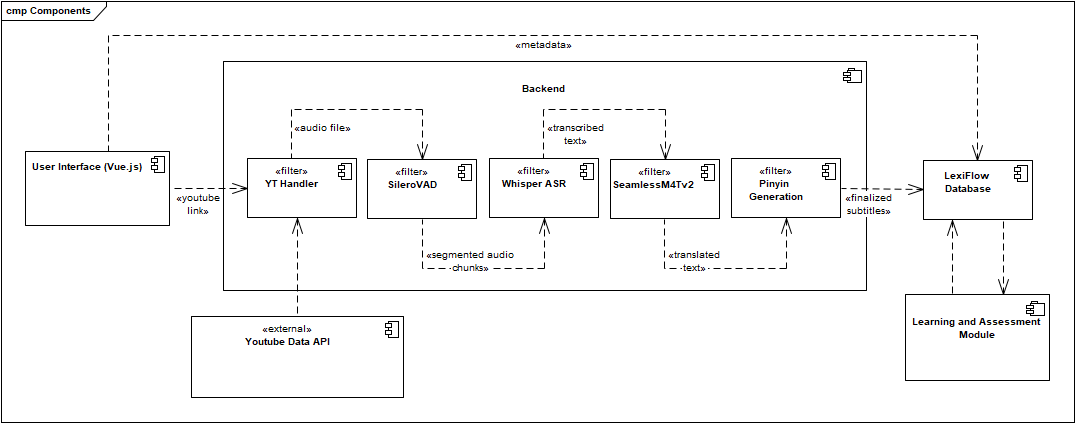
\includegraphics[width=0.95\textwidth]{./figs/arch.png}
    \caption{LexiFlow System Architecture}\label{fig:pipe_and_filter}
    \smallskip
    \begin{flushleft}
        \small * The figure illustrates the Pipe and Filter architecture of LexiFlow, showing the modular processing components and their interactions.
    \end{flushleft}
\end{figure}

\section{Chapter Summary}
Chapter 4 of the thesis discusses the need analysis and system design of the LexiFlow system, which presents an in-depth exploration of the development of a language learning platform. In the first interactive session, the chapter systematically uncovers the needs of the stakeholders, laying the groundwork for the detailed documentation of these requirements in the Software Requirements Specification (SRS, Appendix~\ref{app:srs}) and Software Design Document (SDD, Appendix~\ref{app:sdd}). It also explains about the pipeline architecture approach which is used to build an efficient and scalable system and the user interface design, which is essential for further improving the usability and the system functionality. This systematic approach not only meets the goals of the project, but also gives the project a solid structure for successful implementation and use of LexiFlow. An automated end-to-end test and User Acceptance Testing was then performed to validate the system, and this validation was documented in a Software Test Document as opposed to a separate, standalone Software Test Document, as described in Chapter 5 and Appendices~\ref{app:test-execution-report} and~\ref{app:uat-report}.


\chapter{System Implementation}\label{chap:implementation}

\section{Introduction}
This chapter delves into the actual development of LexiFlow. First I will take you back to the Pipe and Filter design pattern of chapter 4 and demonstrate how it evolved into real code. After that, I stroll through the main learning aspects, subtitle generation, flashcards, quizzes, and crowd-sourcing of error reporting.
\section{Architecture in Practice: Pipe and Filter}Chapter 4 put forward a Pipe and Filter architectural style for the media-processing subsystem. Each stage of subtitle generation is its own filter: it takes the previous stage's output, does its thing, and hands its own output downstream, with no stage aware of anything past its immediate neighbour. Figure~\ref{fig:media_pipeline} shows how this played out. A source video gets downloaded and normalised by FFmpeg, transcribed by a cloud Whisper API, translated by an LLM, then finally annotated with pinyin and HSK levels before it's saved as a subtitle document.

\begin{figure}[H]
    \centering
    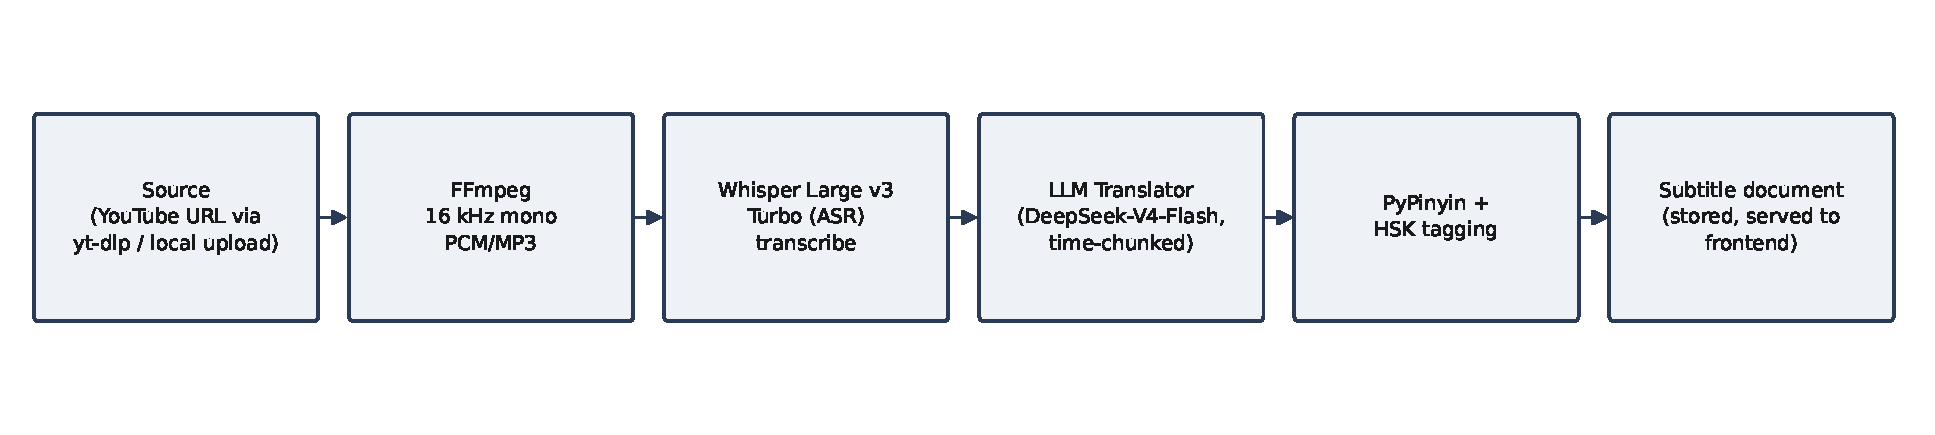
\includegraphics[width=0.95\textwidth]{./figs/fig_media_pipeline.pdf}
    \caption{Pipe and Filter realisation of the media-processing pipeline}\label{fig:media_pipeline}
\end{figure}

Figure~\ref{lst:pipeline} shows the orchestrator that wires these filters together. Every step reports its own progress and elapsed time on its own, and if one step fails, none of the other filters need to know why --- they just don't receive any input.

\begin{figure}[H]
    \begin{verbatim}
async def run_pipeline(job_id, url, is_local=False):
    # 1. Download (yt-dlp) or accept local upload
    file_path = await asyncio.to_thread(download_video, url, job_id)

    # 2. Transcribe (Whisper Large v3 Turbo, FFmpeg-normalised audio)
    transcription = await asyncio.to_thread(api_transcribe, file_path)

    # 3. Translate (LLM, time-chunked) + pinyin/HSK annotation
    translation = await asyncio.to_thread(api_translate, transcription)

    # 4. Post-process into the final subtitle document shape
    end_result = await asyncio.to_thread(api_postprocess, translation)
\end{verbatim}
    \caption{Simplified pipeline orchestrator (\texttt{backend-fastapi/api.py})}\label{lst:pipeline}
\end{figure}

Each filter can be swapped out on its own. The transcription filter, for example, was moved from a locally-hosted Whisper model over to a cloud Whisper API midway through development, and nothing before or after it had to change, since the contract between stages --- a list of timestamped text segments --- stayed the same throughout.

\section{Core Feature: Generate Subtitles (UC06)}

Subtitle generation is the entry point to every other feature in LexiFlow. When a video gets submitted, the \textbf{Whisper Large v3 Turbo} automatic speech recognition model transcribes it, a chat-completion language model translates it sentence-by-sentence into English, and then \textbf{PyPinyin} adds tone-marked pinyin along with per-character HSK difficulty levels. Figure~\ref{lst:translate} shows the translation filter. Segments get batched into five-minute time windows, which gives the model cross-sentence context without risking a truncated response, and the model has to return one JSON translation per input sentence, in order.

\begin{figure}[H]
    \begin{verbatim}
SYSTEM_PROMPT = (
    "...Respond with a JSON object of the exact form "
    '{{"translations": ["...", ...]}} containing exactly '
    "{count} strings, in the same order as the input...")

for chunk in _chunk_by_time(segments, chunk_seconds=300):
    translations = _request_translations(chunk_texts, ...)
    for segment, translated_text in zip(chunk, translations):
        segment["translated_text"] = translated_text
\end{verbatim}
    \caption{Simplified LLM translation filter (\texttt{backend-fastapi/src/llm/translator.py})}\label{lst:translate}
\end{figure}

The subtitle that comes out gets rendered on the watch page as a bilingual, pinyin-annotated transcript synced to the video. And every Chinese token is individually tappable: tap a character or word and you get an instant CC-CEDICT dictionary lookup (Figure~\ref{fig:ss_subtitles}) without playback stopping, which directly fulfils Search Word Definition (UC08) and feeds Save Vocabulary (UC09).

\begin{figure}[H]
    \centering
    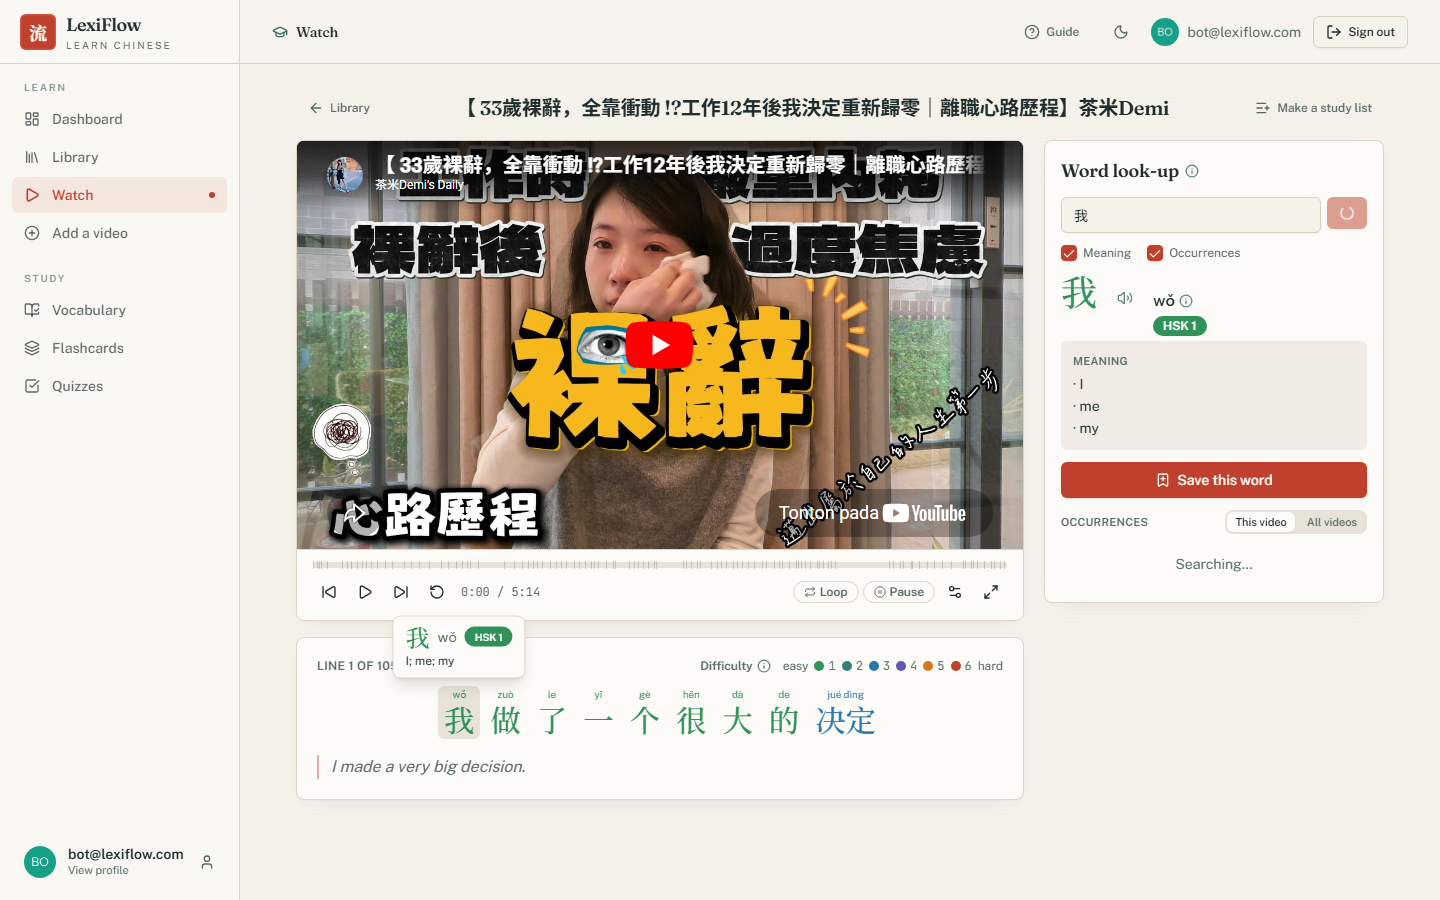
\includegraphics[width=0.7\textwidth]{./figs/fig_ss_subtitles.png}
    \caption{Bilingual subtitle playback with tap-to-look-up dictionary panel}\label{fig:ss_subtitles}
\end{figure}

\section{Core Feature: Generate and Review Flashcards (UC13)}
Saved vocabulary gets reinforced through a spaced-repetition flashcard system built on the \textbf{FSRS (Free Spaced Repetition Scheduler) algorithm}, the same model behind the modern Anki ecosystem. Figure~\ref{fig:fsrs_growth} shows how the scheduled gap for a single item stretches out across successful reviews. Early ones sit a day or two apart. Items you've got down get pushed weeks into the future, so review effort lands where it actually matters. \begin{figure}[H]
    \centering
    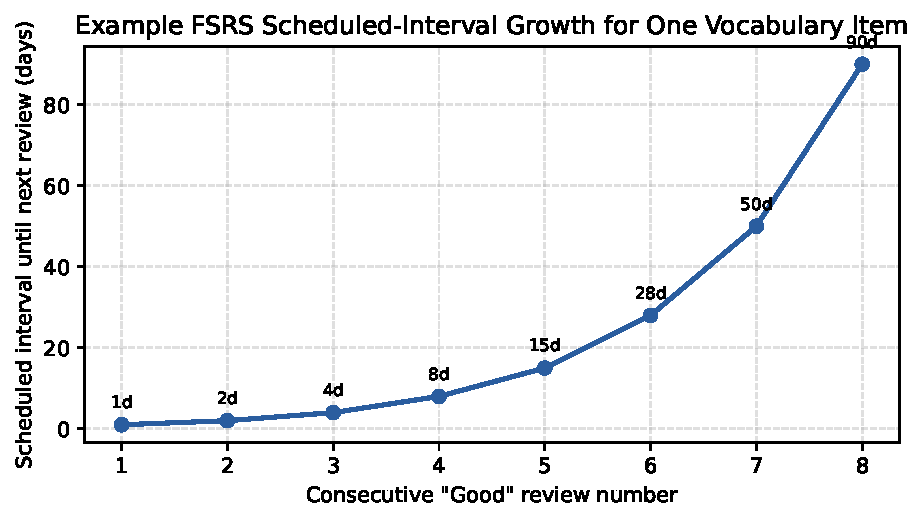
\includegraphics[width=0.7\textwidth]{./figs/fig_fsrs_growth.pdf}
    \caption{Example FSRS scheduled-interval growth for one vocabulary item}\label{fig:fsrs_growth}
\end{figure} Figure~\ref{lst:fsrs} shows the core scheduling function. Each grade (Again/Hard/Good/Easy) recomputes the item's Stability and Difficulty, then works out the next review date straight from the published FSRS weight parameters. We built this in-house rather than leaning on a third-party scheduling service. \begin{figure}[H]
    \begin{verbatim}
function calculateFsrs(card, rating) {
    let { stability, difficulty, state } = card;
    if (card.state === 0 || stability === 0) {
        difficulty = clamp(FSRS_W[4] - FSRS_W[5] * (rating - 3), 1, 10);
        stability  = rating === 1
            ? FSRS_W[0]
            : FSRS_W[1] + FSRS_W[2] * (rating - 2)
                + FSRS_W[3] * Math.pow(rating - 1, 0.5);
    } else {
        const r = Math.pow(1 + 0.1 * (card.elapsedDays / stability), -1);
        difficulty = clamp(difficulty - FSRS_W[6] * (rating - 3), 1, 10);
        stability = /* FSRS stability-growth formula, rating-dependent */ ...;
    }
    const scheduledDays = clamp(Math.round(stability), 1, 365);
    return { stability, difficulty, scheduledDays, nextReviewDate: ... };
}
\end{verbatim}
    \caption{Simplified FSRS scheduler (\texttt{backend-node/.../flashcards.service.js})}\label{lst:fsrs}
\end{figure} The frontend shows this as a flip-style card. The front displays only the Chinese word, and flipping it reveals pinyin and meaning next to the four grading buttons, each labelled with its resulting interval (Figure~\ref{fig:ss_flashcards}) so the learner sees the consequence of their self-assessment right away. \begin{figure}[H]
    \centering
    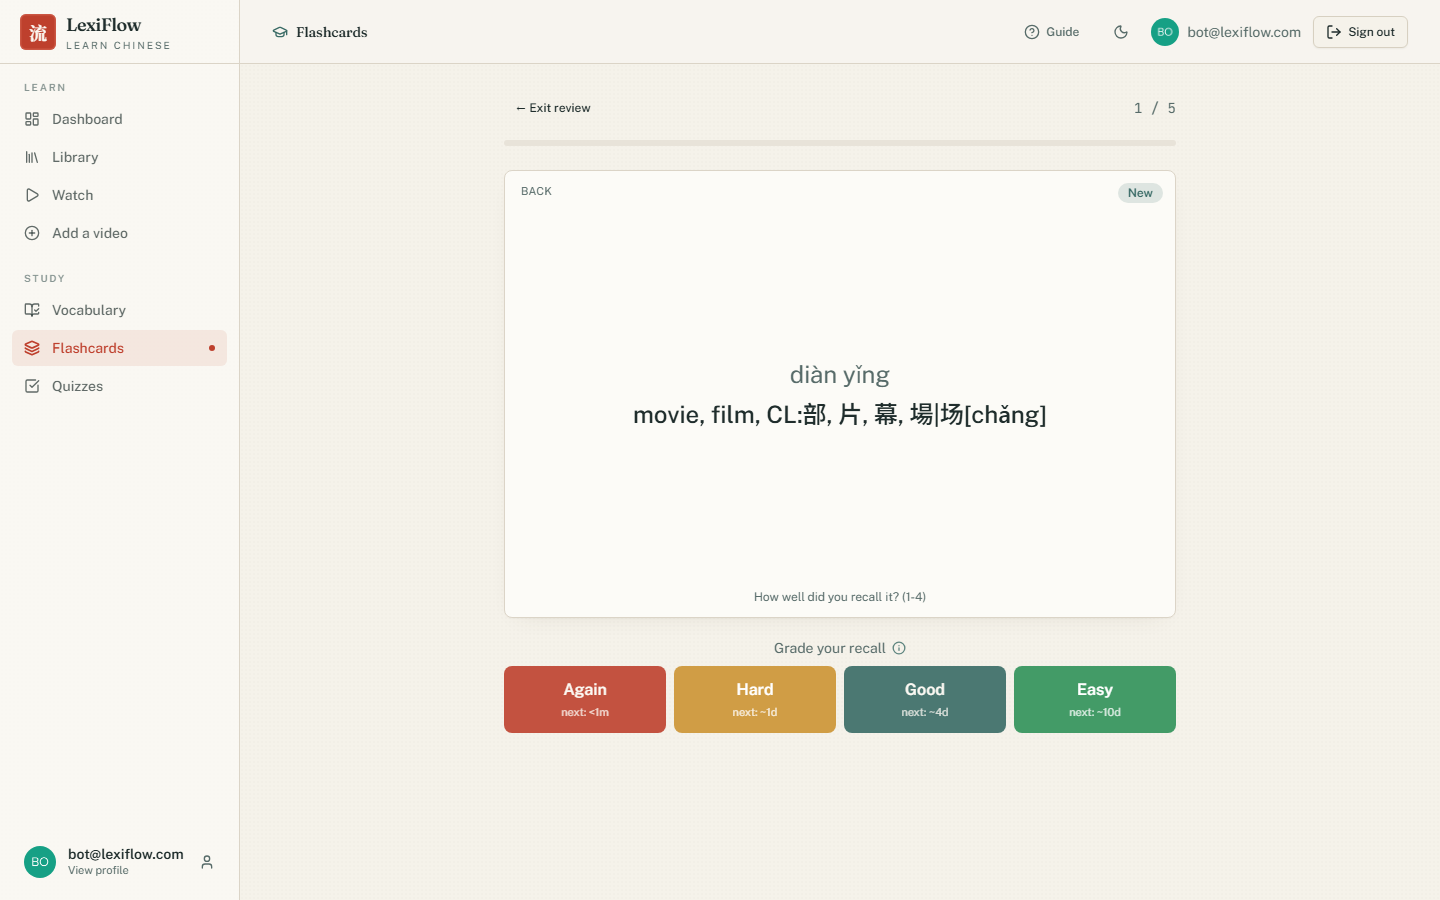
\includegraphics[width=0.7\textwidth]{./figs/fig_ss_flashcards.png}
    \caption{Flashcard review: back face with recall grading buttons}\label{fig:ss_flashcards}
\end{figure}
\section{Core Feature: Generate Quizzes (UC14)}
LexiFlow can whip up a quiz on the fly from any vocabulary list, blending four question types: multiple choice, fill-in-the-blank, true/false, and short answer (Figure~\ref{fig:ss_quizzes}). For fill-in-the-blank, it just masks the target word inside a saved example sentence. Multiple-choice and true/false need something extra, though, plausible wrong answers, the distractors. \begin{figure}[H]
    \centering
    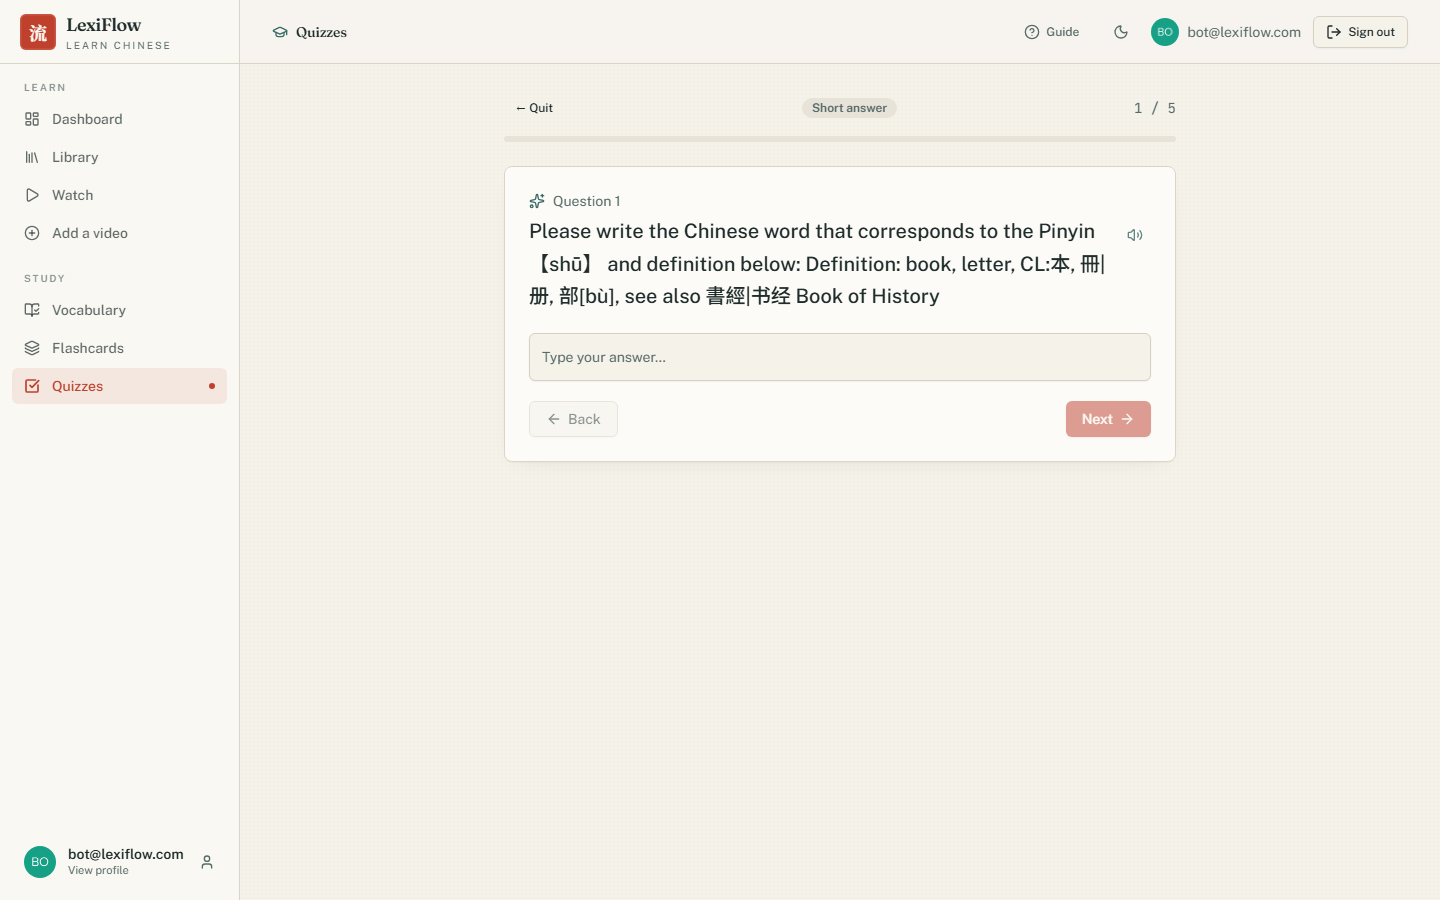
\includegraphics[width=0.7\textwidth]{./figs/fig_ss_quizzes.png}
    \caption{A generated short-answer quiz question}\label{fig:ss_quizzes}
\end{figure} Short-answer responses are trickier. You can't grade them by exact string matching, since one correct answer might be worded a dozen different ways. Figure~\ref{lst:judge} shows the grading filter: an exact match short-circuits right away, and if not, the reference answer and the learner's response both go to an LLM, which has to hand back a structured verdict. \begin{figure}[H]
    \begin{verbatim}
def evaluate_short_answer(self, correct_reference, user_response):
    if ref_clean == resp_clean:
        return {"score": 1.0, "feedback": "Exact", "is_correct": True}

    content = self.provider.chat_complete(
        system=SYSTEM_PROMPT, user=json.dumps({...}), json_mode=True)
    result = json.loads(content)
    return {"score": result["score"], "feedback": result["feedback"],
            "is_correct": result["is_correct"]}
\end{verbatim}
    \caption{Simplified short-answer judge (\texttt{backend-fastapi/services/quiz/judge.py})}\label{lst:judge}
\end{figure} Picking distractors for multiple-choice mixes that same LLM-based plausibility check with two light local heuristics: a pinyin Levenshtein-distance score (catching words that sound alike) and a radical/Unicode similarity score (catching ones that look alike). The three scores get summed, then the top candidates from the same HSK tier win out, so a distractor stays believable without ever sneaking in as an accidental synonym of the right answer.
\section{Core Feature: Crowd-Reporting of Translation Errors (UC11)}
Anyone watching can flag a subtitle line as wrong, picking a category --- translation, pinyin, transcription, or other (Figure~\ref{fig:ss_crowdreport}). Plus but a line only gets bumped up for correction after it clears a deliberately cautious double threshold (Figure~\ref{lst:flag}): at least three different reporters, \emph{and} at least 25\% of everyone who actually saw that line. So one annoyed viewer can't flag stuff on their own. \begin{figure}[H]
    \centering
    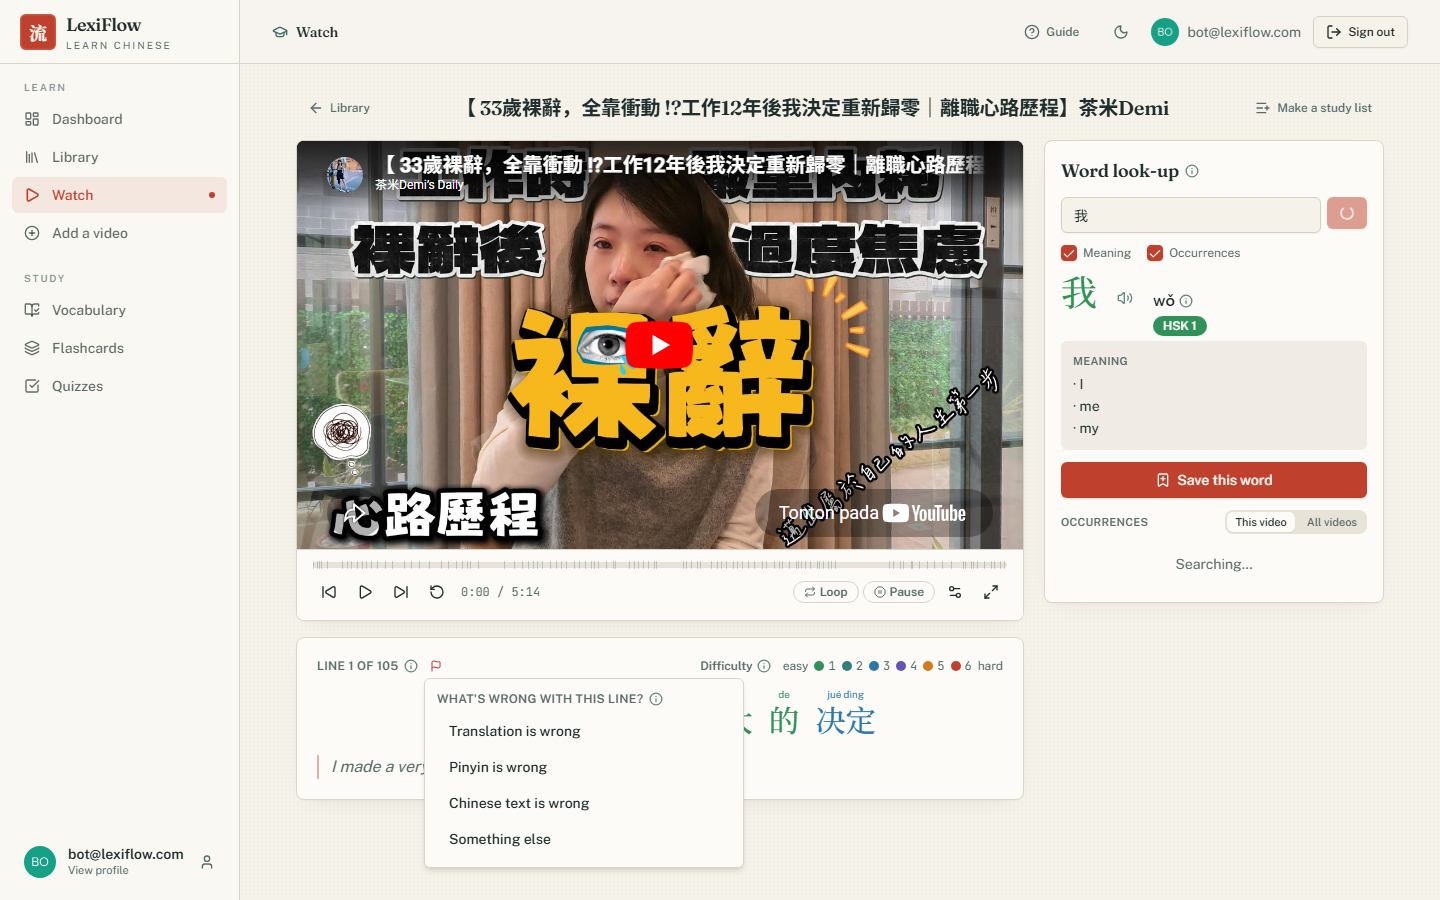
\includegraphics[width=0.7\textwidth]{./figs/fig_ss_crowdreport.png}
    \caption{Reporting a subtitle line and choosing an error category}\label{fig:ss_crowdreport}
\end{figure} \begin{figure}[H]
    \begin{verbatim}
const FLAG_MIN_REPORTS = 3;
const FLAG_THRESHOLD_PERCENT = 0.25;
...
flagged: c.count >= FLAG_MIN_REPORTS
      && (c.count / viewerCount) >= FLAG_THRESHOLD_PERCENT
\end{verbatim}
    \caption{Simplified flag threshold (\texttt{backend-node/.../reports.service.js})}\label{lst:flag}
\end{figure} Once it's flagged, the line gets fixed right away instead of sitting in a queue for a human moderator. The reported segment, three segments of surrounding context, and an instruction tied to the specific error category all get sent to \textbf{Meta's Llama 3.3 70B} model, which is locked to JSON-mode output. Here's the thing --- the original timestamps are always re-applied server-side rather than trusted to the model, so a hallucinated value can't ever knock the subtitle out of sync with the audio, and the fix is saved as a separate, reversible patch instead of overwriting the original transcription.
\section{Core Feature: Browser Extension}
Want LexiFlow's bilingual subtitles on stuff you're already watching? A companion browser extension drops graded Chinese subtitles, word lookup, and text-to-speech right onto the YouTube player. No more copying video URLs into the main platform first. \begin{figure}[H]
    \centering
    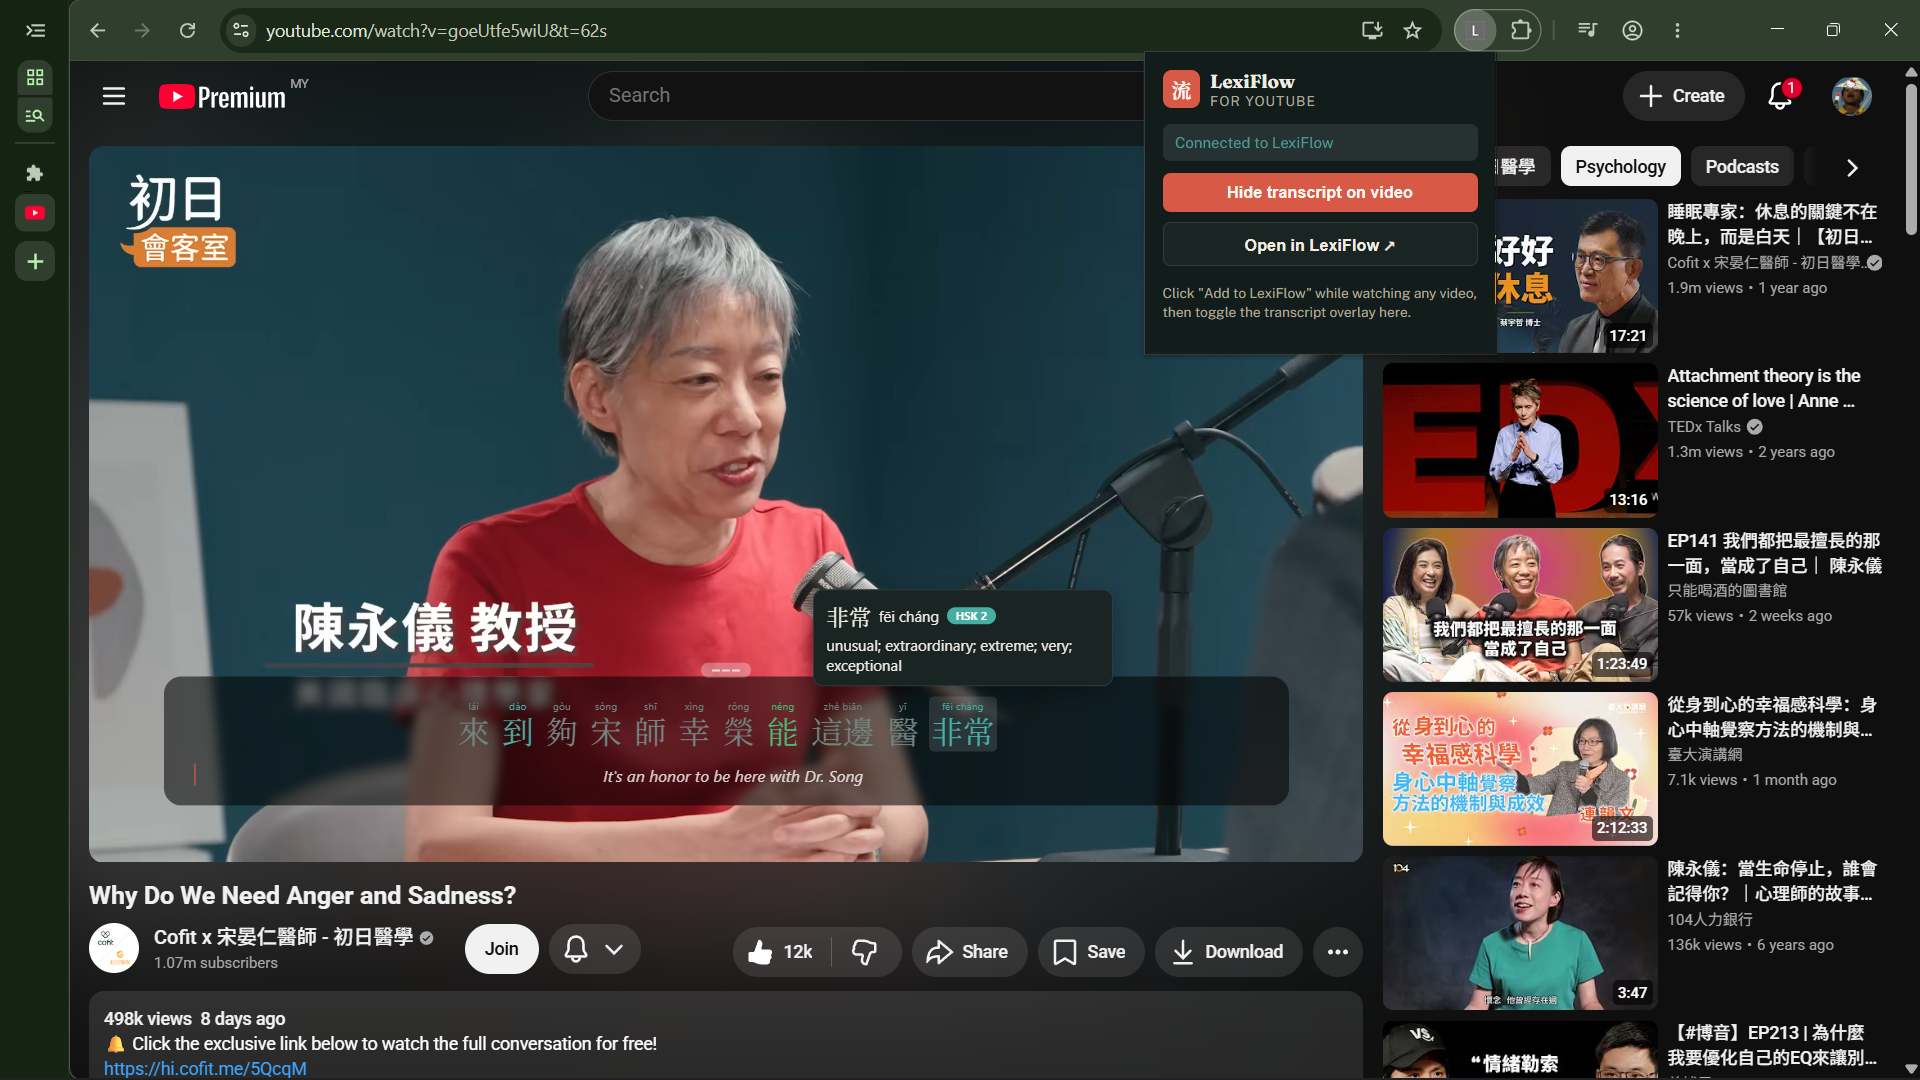
\includegraphics[width=0.95\textwidth]{./figs/fig_browser_extension.png}
    \caption{LexiFlow browser extension overlay on YouTube}\label{fig:ss_extension}
\end{figure}
\section{DevOps and Deployment}
Figure~\ref{fig:deployment_topology} lays out where each piece of the system actually lives. But the frontend's a static build, served off \textbf{Vercel}'s edge CDN. The Node.js backend, the FastAPI worker, and PostgreSQL all sit together on one \textbf{Tencent Cloud Lighthouse} VM through Docker Compose, with a \textbf{SaladPool} instance kept around as a rarely-touched failover worker. On every push to \texttt{main}, \textbf{GitHub Actions} builds and pushes a container image to GHCR, then redeploys the VM on its own---so there's no manual deployment step. All AI inference---transcription, translation, quiz grading, segment correction---gets handed off to externally hosted language models (Whisper Large v3 Turbo, DeepSeek-V4-Flash, and Llama 3.3 70B), which means the deployment needs no GPU. \begin{figure}[H]
    \centering
    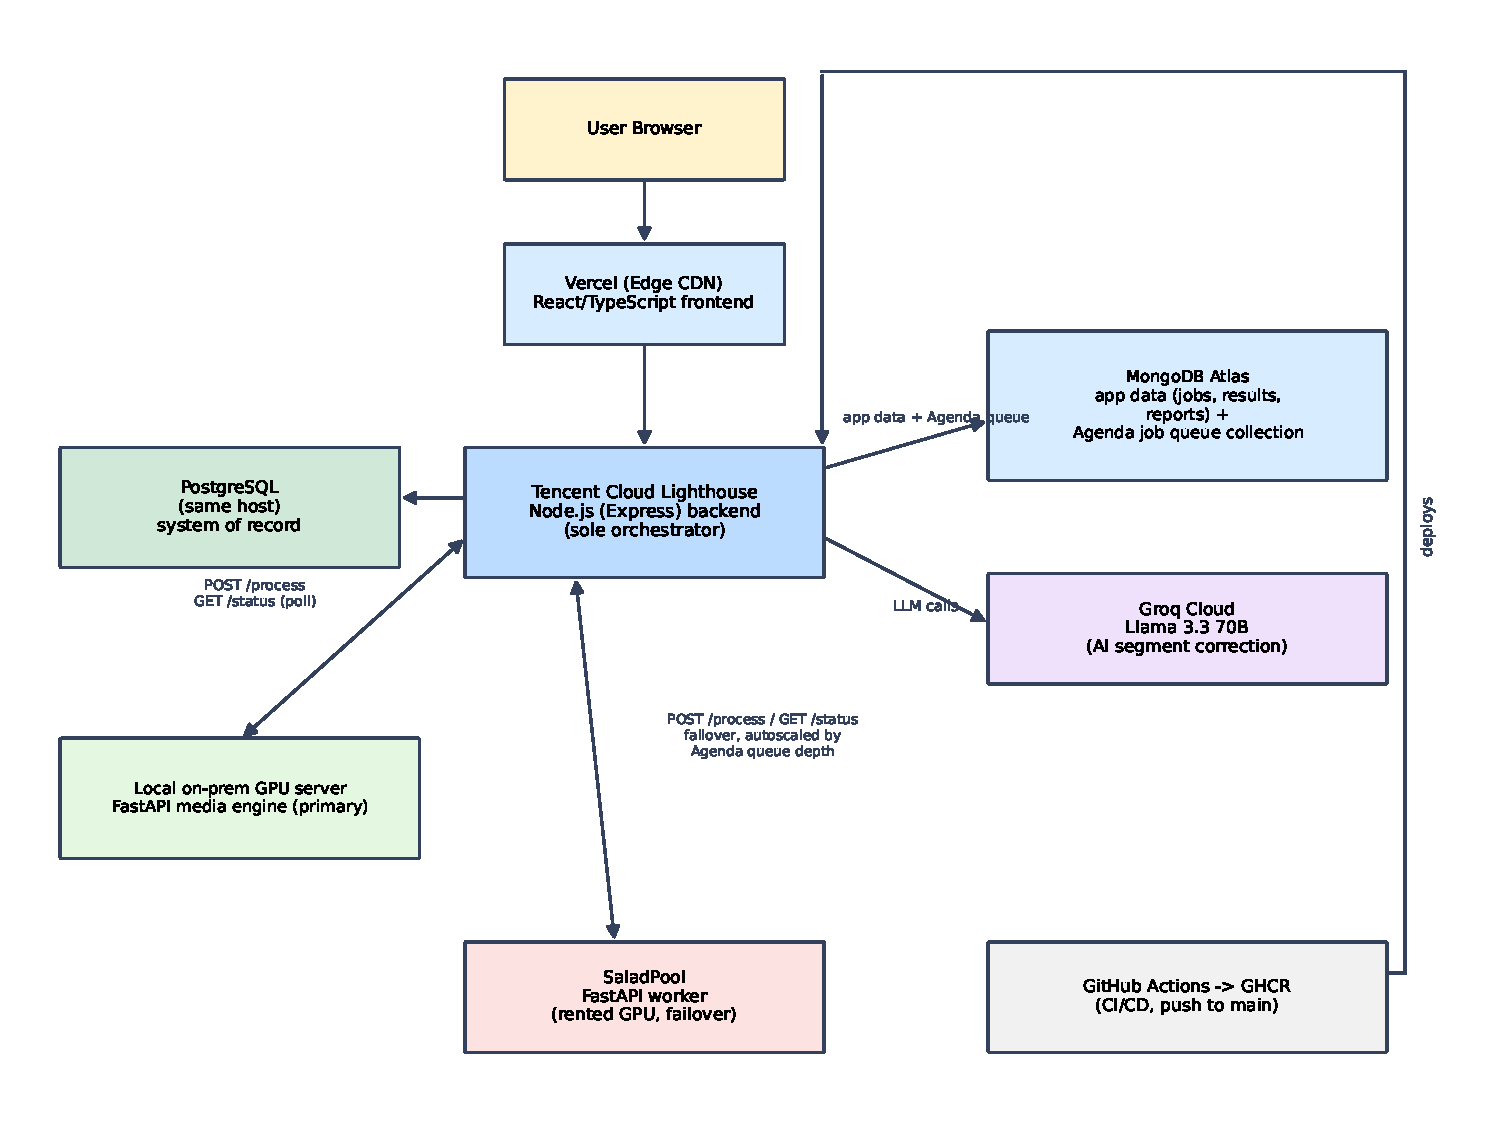
\includegraphics[width=0.95\textwidth]{./figs/fig_deployment_topology.pdf}
    \caption{LexiFlow deployment topology}\label{fig:deployment_topology}
\end{figure}
\section{Verification and Validation}
The system was checked two different methods. The first was an automated end-to-end Playwright suite which was executed directly against the live test deployment from UC01-04 to UC13-14. Of 30 test cases, we had 25 passed, 4 failed, and 1 known skip. It wasn't because of any problem with the test scripts, it was because of two real, reproducible defects, one was the onboarding tour which you couldn't dismiss and the other was a missing single-page-application fallback route. Further details of the methodology, per test-case results and root cause analysis are provided in Appendix~\ref{app:test-execution-report}. Then came User Acceptance Testing, conducted with four users, representing four user groups identified in Chapter 4: a Mandarin learner who has been having trouble with the language, a self-directed language learner who requires some domain-specific vocabulary, a native speaker reviewer to ensure the correctness of the transcription and translation, and the instructor stakeholder. They returned feedback on the merit of the Tap-to-Look-Up, Vocabulary-Saving, and Quiz-Generation flows. It also brought two honest problems to the fore for later: the lack of accuracy when compared to commercial-grade captioning and the lack of classroom-management features, both of which were not functional requirements in Chapter 4. Full participant profiles, scenarios and acceptance-criteria analysis is found in Appendix~\ref{app:uat-report}.
\section{Chapter Summary}
So in this chapter we've seen how the Pipe and Filter architecture described in Chapter 4 transit to being a pipeline that can be swapped out independently, and then explored the four primary learning features, subtitle generation, flashcards, quizzes, and a crowdsourced corrections. Each one combines a deterministic local algorithm (FSRS, threshold checks, pinyin/visual similarity) with an LLM only when there is open ended judgement. The intent was for deployment to remain light, all the AI inference was handed over to external APIs. By automated end-to-end testing and User Acceptance Testing, we confirmed the entire item, and we found all the defects we could, which all went back to one specific, repeatable root cause, and not to some architectural defect.

\chapter{CONCLUSION}
\section{Introduction}
In this chapter, LexiFlow's development, its output, and the extent to which the project fell short or met its initial objectives are covered. I will concentrate on the results, the successes to talk about and a couple areas that may need improvement later on. In short, an examination of the success of how LexiFlow in fact addressed teachers' and students' concerns and future directions and growth potential for the program. The project managed to deliver something solid – a language learning system that really fulfilled what users wanted. The architecture and tech decisions are along the way too? They are good building blocks for the next steps. Through continuous development and refinement, LexiFlow may become one of the more successful language learning programs available, for universities and beyond, both dependable and user-friendly.

\section{Achievement of Project Objectives}The LexiFlow project had four main goals, which was specified in Section~\ref{sec:obj} of this paper.  They were all designed to make language learning easier.

\begin{enumerate}[label= (\alph*)]
    \item \textbf{Elicit full Requirements from Stakeholders:} The first goal was to get a complete list of Requirements from Stakeholders. They did this by interviewing them in a round-robin fashion. During those discussions, I really got a feeling for what language-learning issues people face and how many problems they have to solve around language use across the UTM community. The requirements that I collected became functional and non-functional specifications for the project. All that is documented in the Software Requirements Specification (SRS) in Appendix~\ref{app:srs}. So this is one we've done, requirements picked up and analyzed properly.
    \item \textbf{Design a Web-Based Platform:} The second objective was to design a Web Based Platform with an appropriate architecture behind it. LexiFlow designed around Pipe \& Filter architecture model. Vue for the front end allowed me to create a user friendly and responsive interface, and on the back end, I used Python and NodeJS. The entire detailed design and documentation for the system is contained in the Software Design Document (SDD) (see Appendix~\ref{app:sdd}). So there is one more that got accomplished!
    \item \textbf{Develop the Full Platform:} The third was to create the language learning platform itself – the Full Platform. This involved assembling the audio processing system, including voice activity detection, automatic speech recognition, translation and generation of the pinyin. All the features were straight out of the requirements I had gathered and the design specifications.
    \item \textbf{Evaluate and Test the Functionality:} The final objective was to assess and test the functionality of LexiFlow – how well it actually enhances the language learning experience. In the next phase, PSM2, that will be done in the form of heavy testing, unit tests, integration tests and user acceptance tests. The preliminary test cases and test approaches are already included in the Software Testing Documentation (Appendix~\ref{app:std}). This objective is marked as complete when the project is developed and testing has been completed.
\end{enumerate}
\section{Service Enhancement and Practical Value}So LexiFlow does more than just hit the goals it set out to. It has a score on two of the three dimensions that people tend to use to determine whether a system is in fact useful: it improves the service, and it improves the lives of the people who use it. Commercial value? Not yet, no one has tried a pricing model, payment structure or any actual testing on the market. Here's how it enhances the quality of service. That was the painful thing that the stakeholder interview (Appendix~\ref{app:stakeholder-interview-questions}) raised was that each of the 3-minute clips of authentic Mandarin content took 10 to 30 minutes of hand work to transcribe, translate and annotate with pinyin. That becomes a pipeline that a learner and/or teacher can fire off whenever they want, and a crowd-correction feature allows for ongoing improvement without anyone having to redo that grind. Such a change from the stakeholder description where there was very little authentic content used because of the high cost of preparing it. The side of Quality of Life was confirmed independently during UAT (Appendix~\ref{app:uat-report}). One of the students in difficulty surmised that this platform would have pushed them a little closer to their real exam mark. A Mandarin speaker in a Mandarin-speaking environment described it as a daily go-to for them to reduce the amount of "real" misunderstandings in the workplace. They had never encountered those problems in classroom activities or with any generic apps or textbooks. These are not the "understood benefits" that are assumed, but the benefits that users reported they felt they had gained, in their own learning, and in their general confidence speaking with people.
\section{Suggestions for Future Improvement}So, building on what we learned from automated testing and UAT, here's what I'd recommend fixing in future versions of LexiFlow. First is the two known defects from test execution. The onboarding tour you can't ignore (LF-BUG-01) and a missing SPA fallback route, which results in a raw 404 when handling directly to a URL (LF-BUG-02). They both need to be addressed before moving into any production rollout: one of them prevents core navigation for first time visitors, while the other does for returners. Secondly, there is the difference in accuracy that our native-speaker UAT participant pointed out between the accuracy of the faster-whisper in LexiFlow's self-hosted pipeline compared to that of the commercial-grade auto-captioning on YouTube. That should narrow down further. The crowd-reporting/AI-assisted correction feature already built-in Chapter 5 is configured beautifully for exactly that in the long term and, making a long-term call here, it's worth measuring the effectiveness first-hand, in a later round of evaluation. Third and this is the big one. A classroom-management module. Something that enables one to start a class, upload certain videos or quizzes for a class, and view a progress dashboard that shows how far along a lecturer is in each of their students. It was a big unmet need by the instructor stakeholders during UAT and was not a part of the initial functional needs, it is therefore a no-brainer for the next phase. Beyond the aforementioned evidence-based priorities, is the decision to replace the large multilingual model with a lighter Mandarin local model, reducing processing time and server VRAM and thus reducing operating costs. The reduction in runtime and resources would be further achieved by adopting leaner runtimes such as ONNX or TensorRT. All these changes combined would make LexiFlow more precise, more convenient for institutions and more economical to operate.

\bibliographystyle{unsrtnat} % Use the "abbrvnat" BibTeX style for formatting the bibliography
\bibliography{reference} % Entries are in the refs.bib file

\appendix



% \chapter{List of Prompts Used}
% \pdfbookmark[0]{List of Prompts Used}{sec:list-of-prompts-used}
% 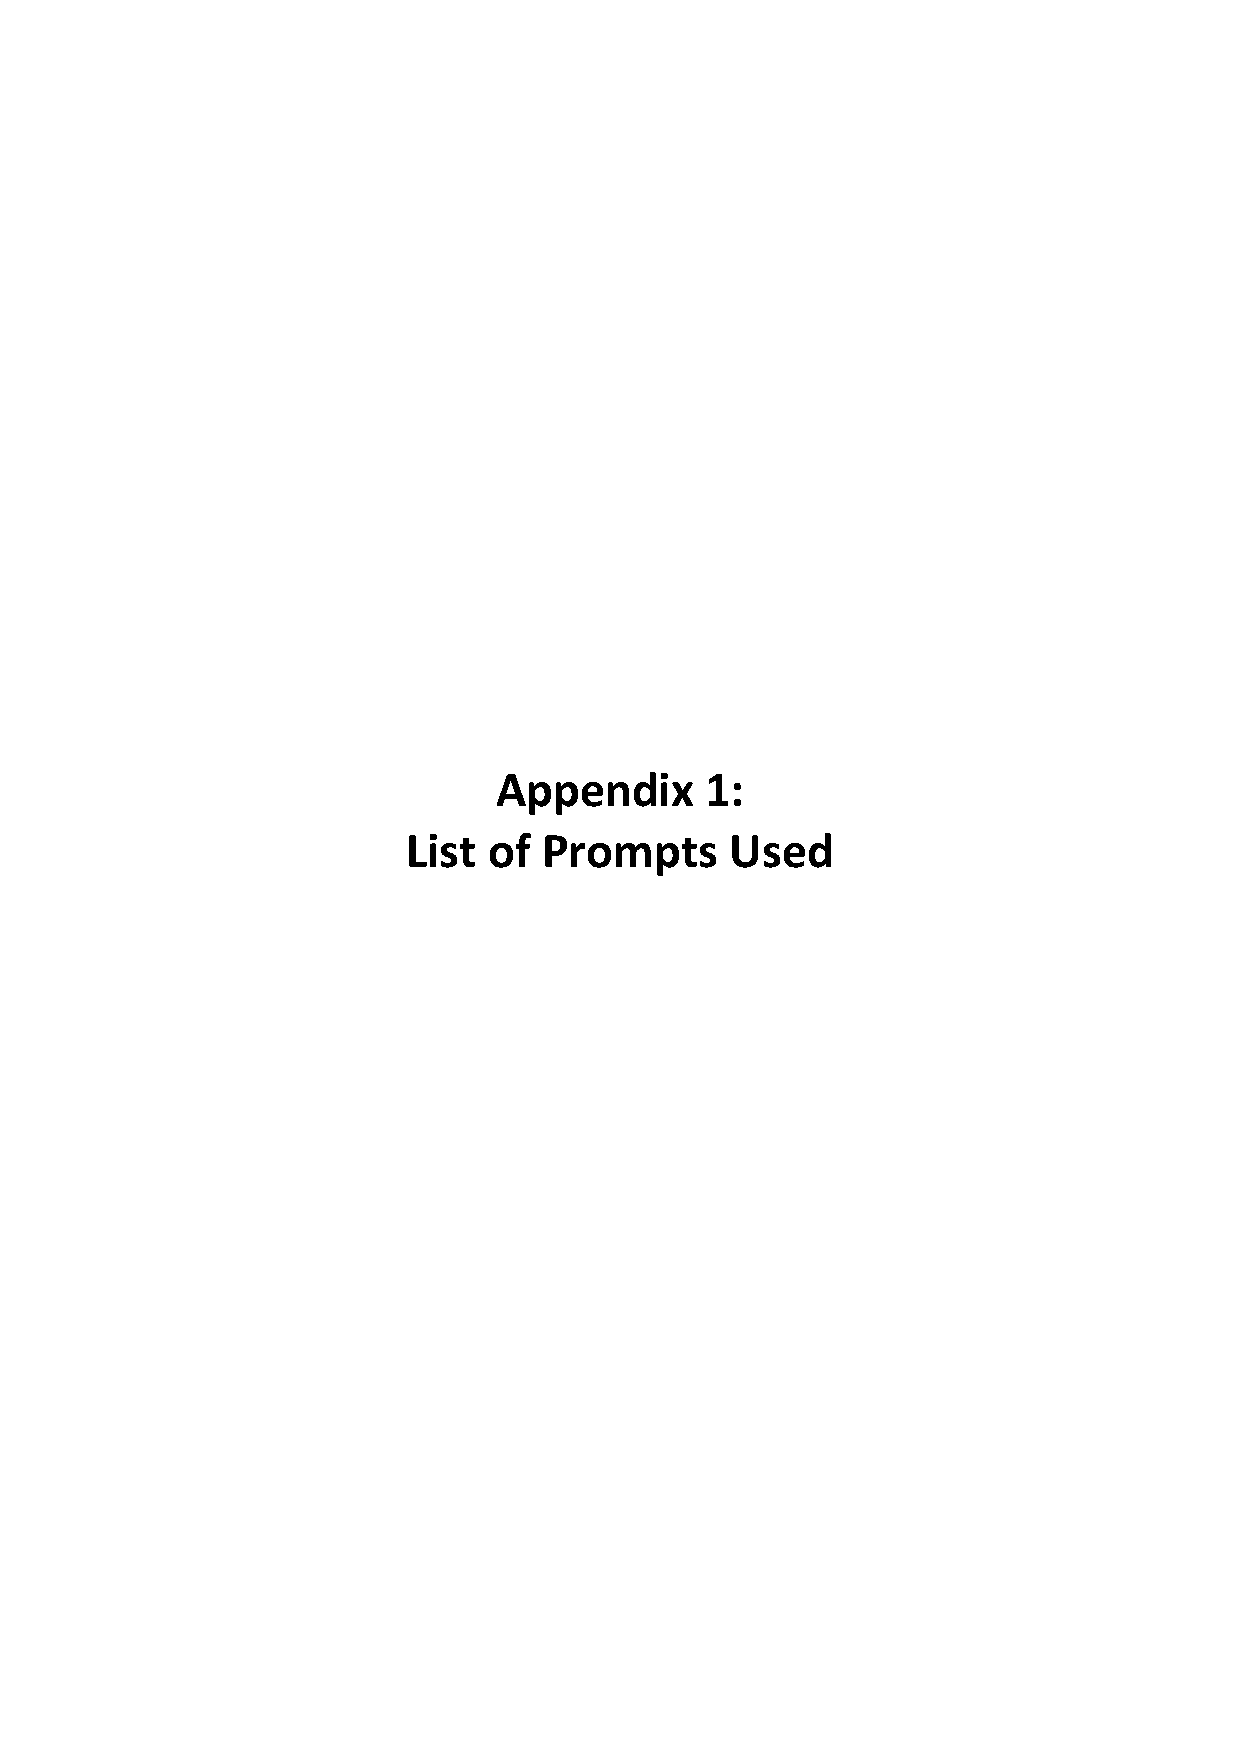
\includepdf[pages=-]{figs/prompts.pdf}

% \chapter{Test Execution Report}\label{app:test-execution-report}
% \pdfbookmark[0]{Test Execution Report}{sec:test-execution-report}
% 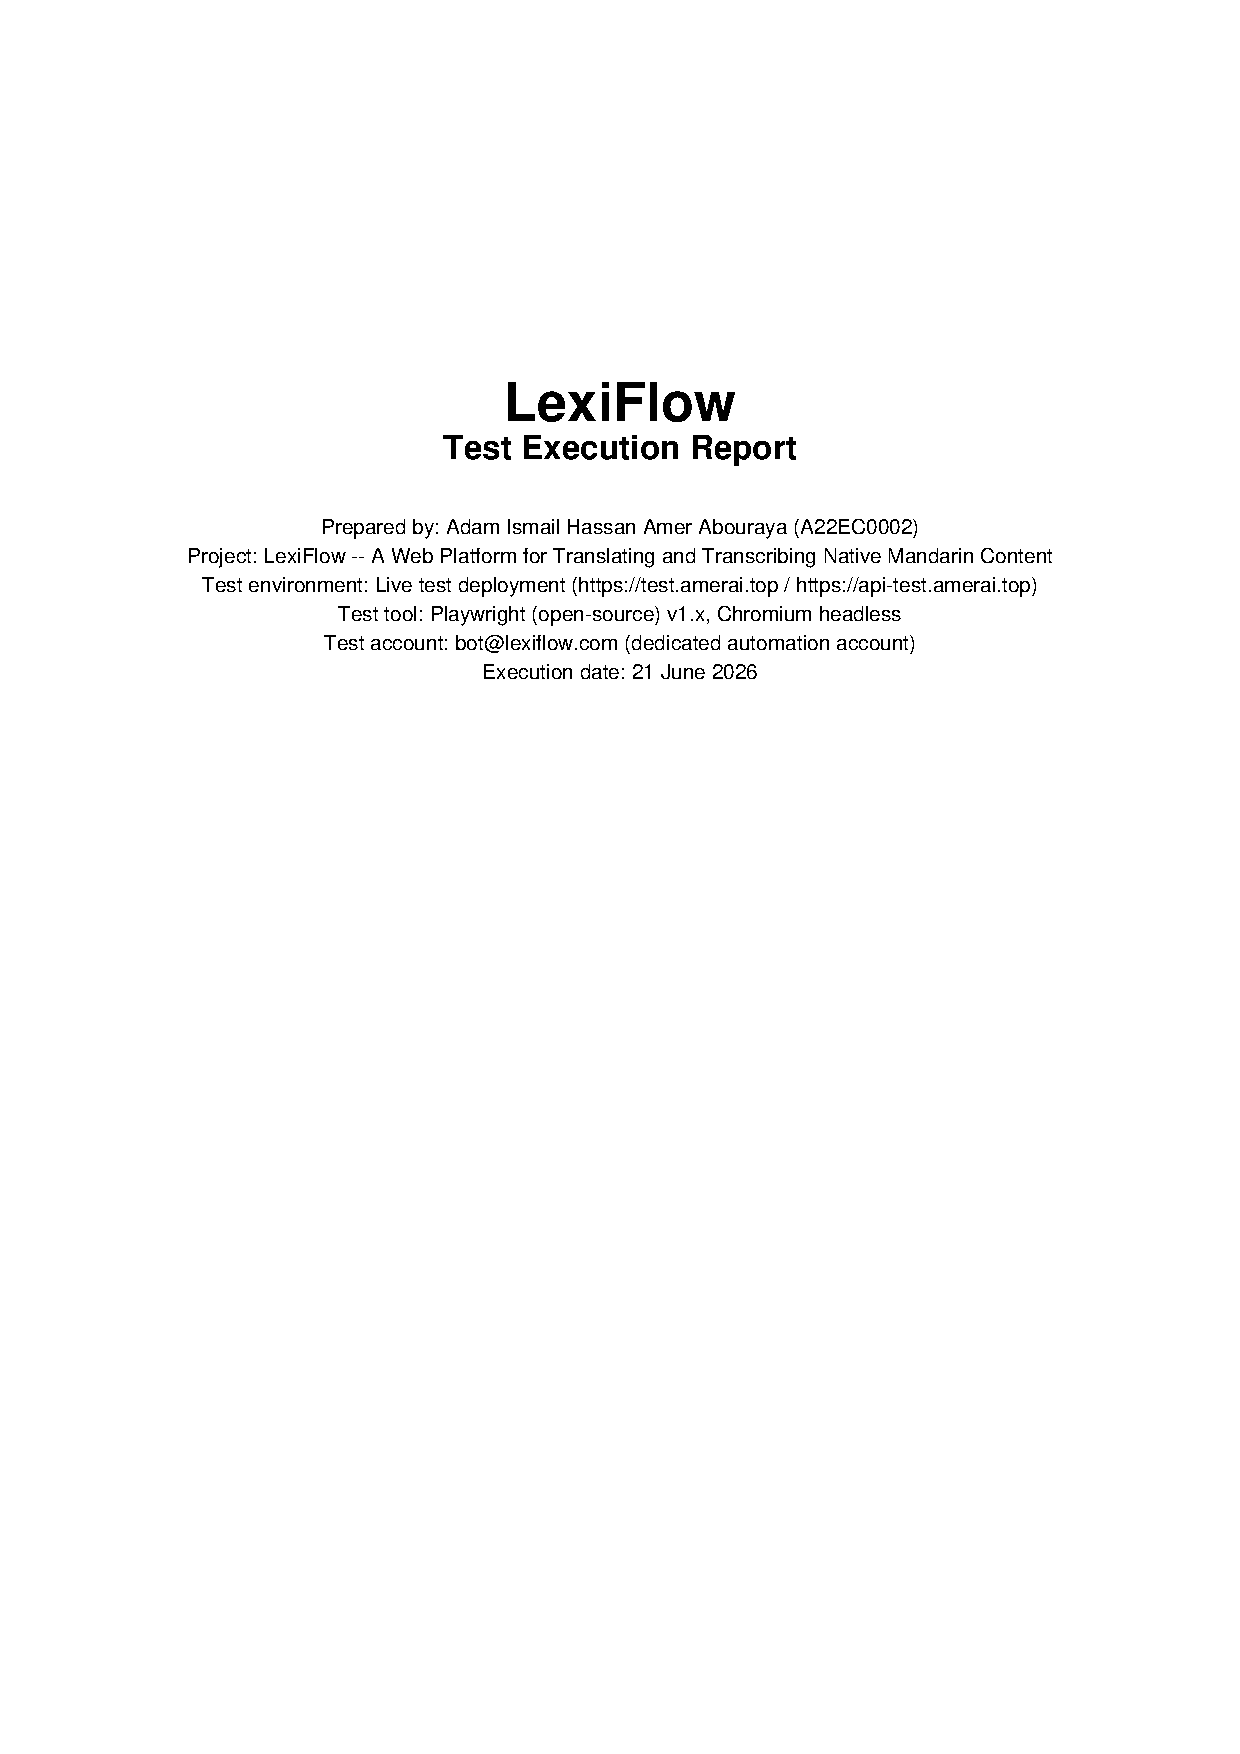
\includepdf[pages=-]{figs/test_execution_report.pdf}

% \chapter{User Acceptance Test (UAT) Report}\label{app:uat-report}
% \pdfbookmark[0]{User Acceptance Test (UAT) Report}{sec:uat-report}
% 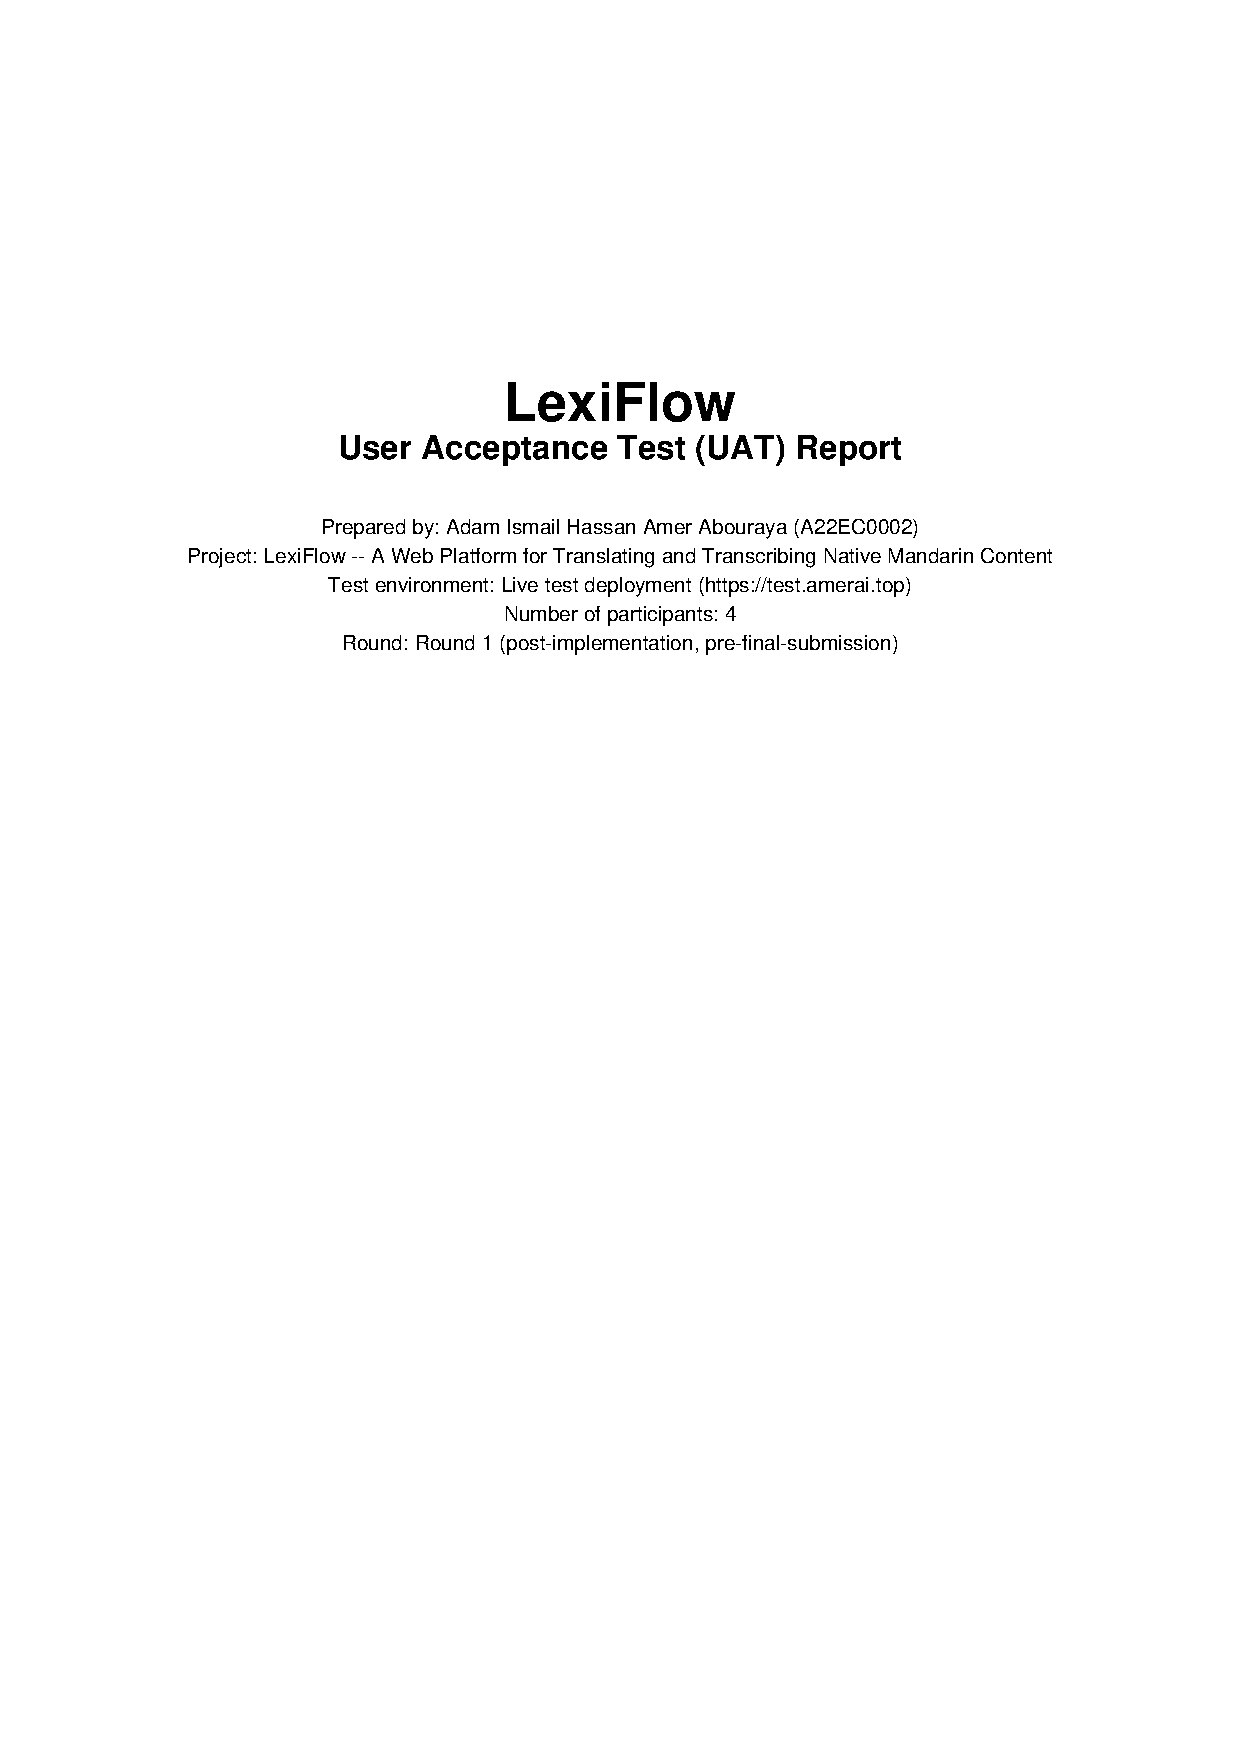
\includepdf[pages=-]{figs/uat_report.pdf}

% \chapter{Stakeholder Interview Questions}\label{app:stakeholder-interview-questions}
% \pdfbookmark[0]{Stakeholder Interview Questions}{sec:stakeholder-interview-questions}


% \section{Teaching Context \& Methods}
% \noindent How many students do you typically teach per semester?\\
% =\textgreater{} around 180–200 students


% \noindent What proficiency levels do you teach (beginner, intermediate, advanced)? What is their HSK level?\\
% =\textgreater{} all classes here in UTM language academy teach beginner level Mandarin. The student reaches HSK 1 by the time they finish the subject.

% \noindent How do you currently incorporate authentic content into your curriculum? \\
% =\textgreater{} as support material. After finishing the lesson slides. The students watch a video or two. The videos are usually kindergarten songs.

% \noindent What challenges do you face when preparing authentic content materials?\\
% =\textgreater{} the biggest challenge is to find material with the correct level for the students. If it is too difficult or too simple then the students will not learn much.

% \section{Content Processing \& Management}
% \noindent  How much time do you spend creating subtitles/transcriptions for videos?\\
% =\textgreater{} 10–30 mins for simple 3-minute videos

% \noindent What types of authentic content work best for different proficiency levels?\\
% =\textgreater{} for beginner levels, kindergarten songs are the best choice. However, a lot of students find them childish or boring. Movies are great for more advanced levels. Travel vlogs are also a nice content for beginner/ intermediate levels.

% \noindent How do you currently assess student comprehension of authentic materials?\\ =\textgreater{} by using quizzes. Both in class and online quizzes on e-learning. Listening quizzes are the best but mcq is also usable.

% \section{Quality \& Accuracy Requirements}
% \noindent What level of transcription accuracy is acceptable for educational use?\\
% =\textgreater{} above 90\% is acceptable

% \noindent What quality control measures should be in place?\\
% =\textgreater{} as long as the model or translation service used is backed by good research then this should good enough for such projects

% \noindent How important is consistency in pinyin romanization systems?\\
% =\textgreater{} it is important but not the most important part of this system. Having correct translation is the most important feature in this system.

% \chapter{Feedback on Prototype Meeting with Stakeholder}\label{app:feedback-on-prototype}
% \pdfbookmark[0]{Feedback on Prototype Meeting with Stakeholder}{sec:feedback-on-prototype}

% Saya telah pun mengadakan pertemuan dengan Adam. Beliau telah membentangkan prototype tersebut.~\href{https://lexiflow.amerai.top}{[Prototype Link]}.

% \section{Maklumbalas saya adalah seperti berikut:}

% \begin{enumerate}[label=\arabic*.]
%     \item Secara keseluruhannya sistem tersebut berfungsi dengan baik.
%     \item Hasil transcribing video yang ditunjukkan adalah tepat, melebihi 95\%.
%     \item Ketepatan terjemahan juga adalah melebihi 90\%.
%     \item Features seperti terjemahan per kosa kata adalah tepat dan membantu.
%     \item Setiap kosa kata mempunyai label tahap HSK (Chinese Proficiency Test), ia membantu untuk rujukan pengguna.
%     \item Sistem tersebut sangat mudah untuk digunakan.
%     \item Prototype ini sesuai untuk digunakan untuk pengajar dan pelajar bagi tujuan pembelajaran bahasa mandarin.
% \end{enumerate}

% \section{Terdapat 2 masalah utama:}

% \subsection{Terjemahan}
% \begin{enumerate}[label=\arabic*.]
%     \item Ketepatan terjemahan terganggu pada video yang mempunyai kandungan bahasa rojak (Mandarin-English, Mandarin-Malay).
%     \item Frasa yang mempunyai maksud tersirat atau bergantung pada konteks budaya sedikit mempengaruhi ketepatan terjemahan.
%     \item Kata ulangan (bentuk jamak) sering terlepas untuk ditranskrip secara penuh, namun ia tidak mengganggu terjemahan ayat secara keseluruhannya.
% \end{enumerate}

% \subsection{Kegagalan Transcribing}
% Kami mendapati terdapat video yang tidak berjaya untuk transcribe. Kami menjangkakan terdapat beberapa sebab:
% \begin{enumerate}[label=\arabic*.]
%     \item Suara talent yang bercakap tidak jelas atau tidak kuat.
%     \item Berlaku code-switching (Mandarin-English-Malay) yang terlalu kerap.
%     \item Talent bercakap terlalu laju.
% \end{enumerate}

% \section{Cadangan dan Penambahbaikan:}
% \begin{enumerate}[label=\arabic*.]
%     \item Perlu uji lebih banyak video yang mempunyai slang atau dialect yang berbeza.
%     \item Feature "Recommended Videos" perlu di label mengikut kesesuaian tahap penguasaan bahasa pengguna.
%     \item Penambahan features untuk penilaian pengguna, seperti flashcard, quiz dan lain-lain.
%     \item Sekiranya tujuan utama sistem ini adalah untuk pembelajaran, tambah features playlists yang bertema bagi memastikan pembelajaran lebih tersusun dan berstruktur.
% \end{enumerate}

% \begin{flushleft}
%     \textbf{MUHAMMAD ZAID BIN MUHAMMAD SHAFIE} \\
%     Foreign Language Coordinator \\
%     Mandarin Language Instructor \\
%     Language Academy \\
%     Faculty of Social Sciences and Humanities \\
%     UTM, Johor Bahru \\
%     Email: m.zaid@utm.my
% \end{flushleft}


% \chapter{Project Timeline Management with Jira}\label{app:project-timeline-management-with-jira}
% \pdfbookmark[0]{Project Timeline Management with Jira}{sec:project-timeline-management-with-jira}

% \chapter{Software Requirements Specification (SRS)}\label{app:srs}
% \pdfbookmark[0]{SRS}{sec:srs}
% 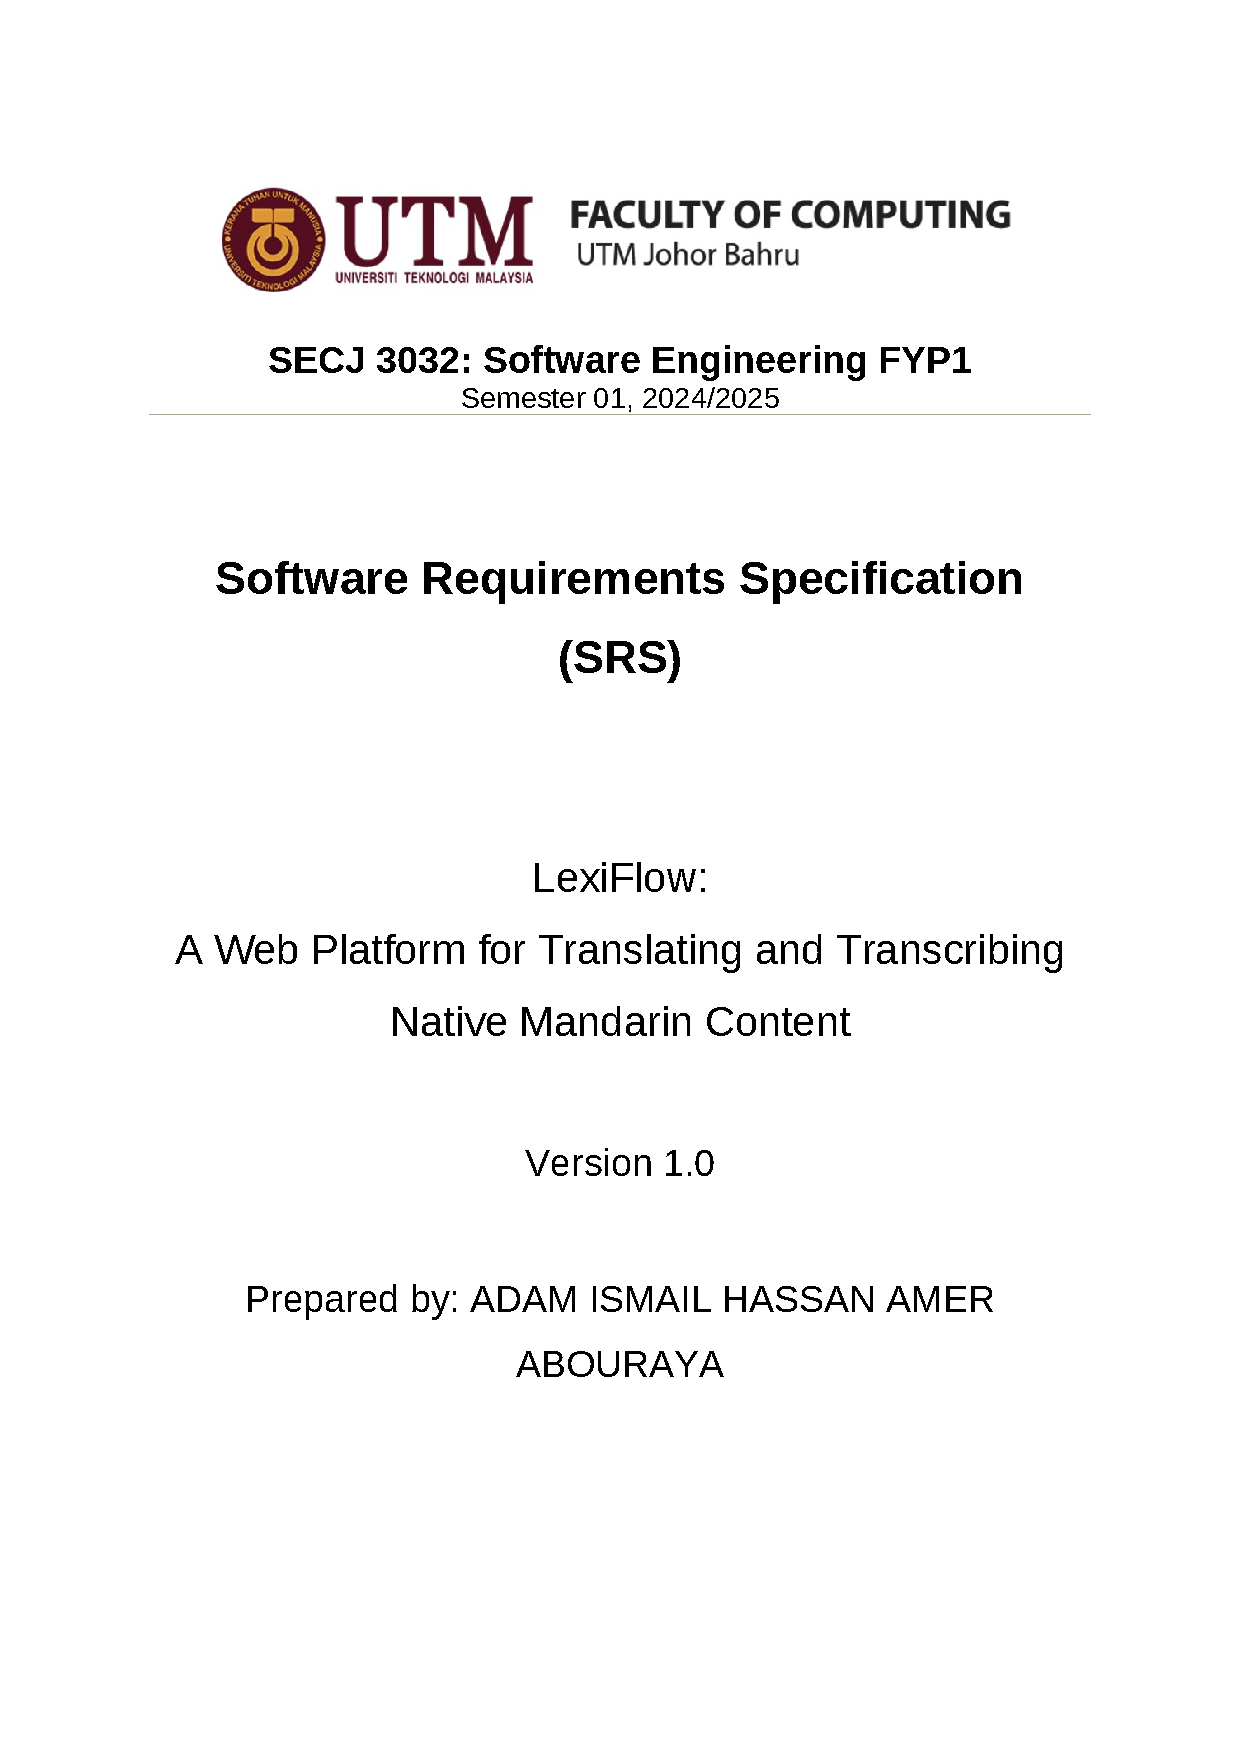
\includepdf[pages=-]{figs/srs.pdf}
% \chapter{Software Design Document (SDD)}\label{app:sdd}
% \pdfbookmark[0]{SDD}{sec:sdd}
% 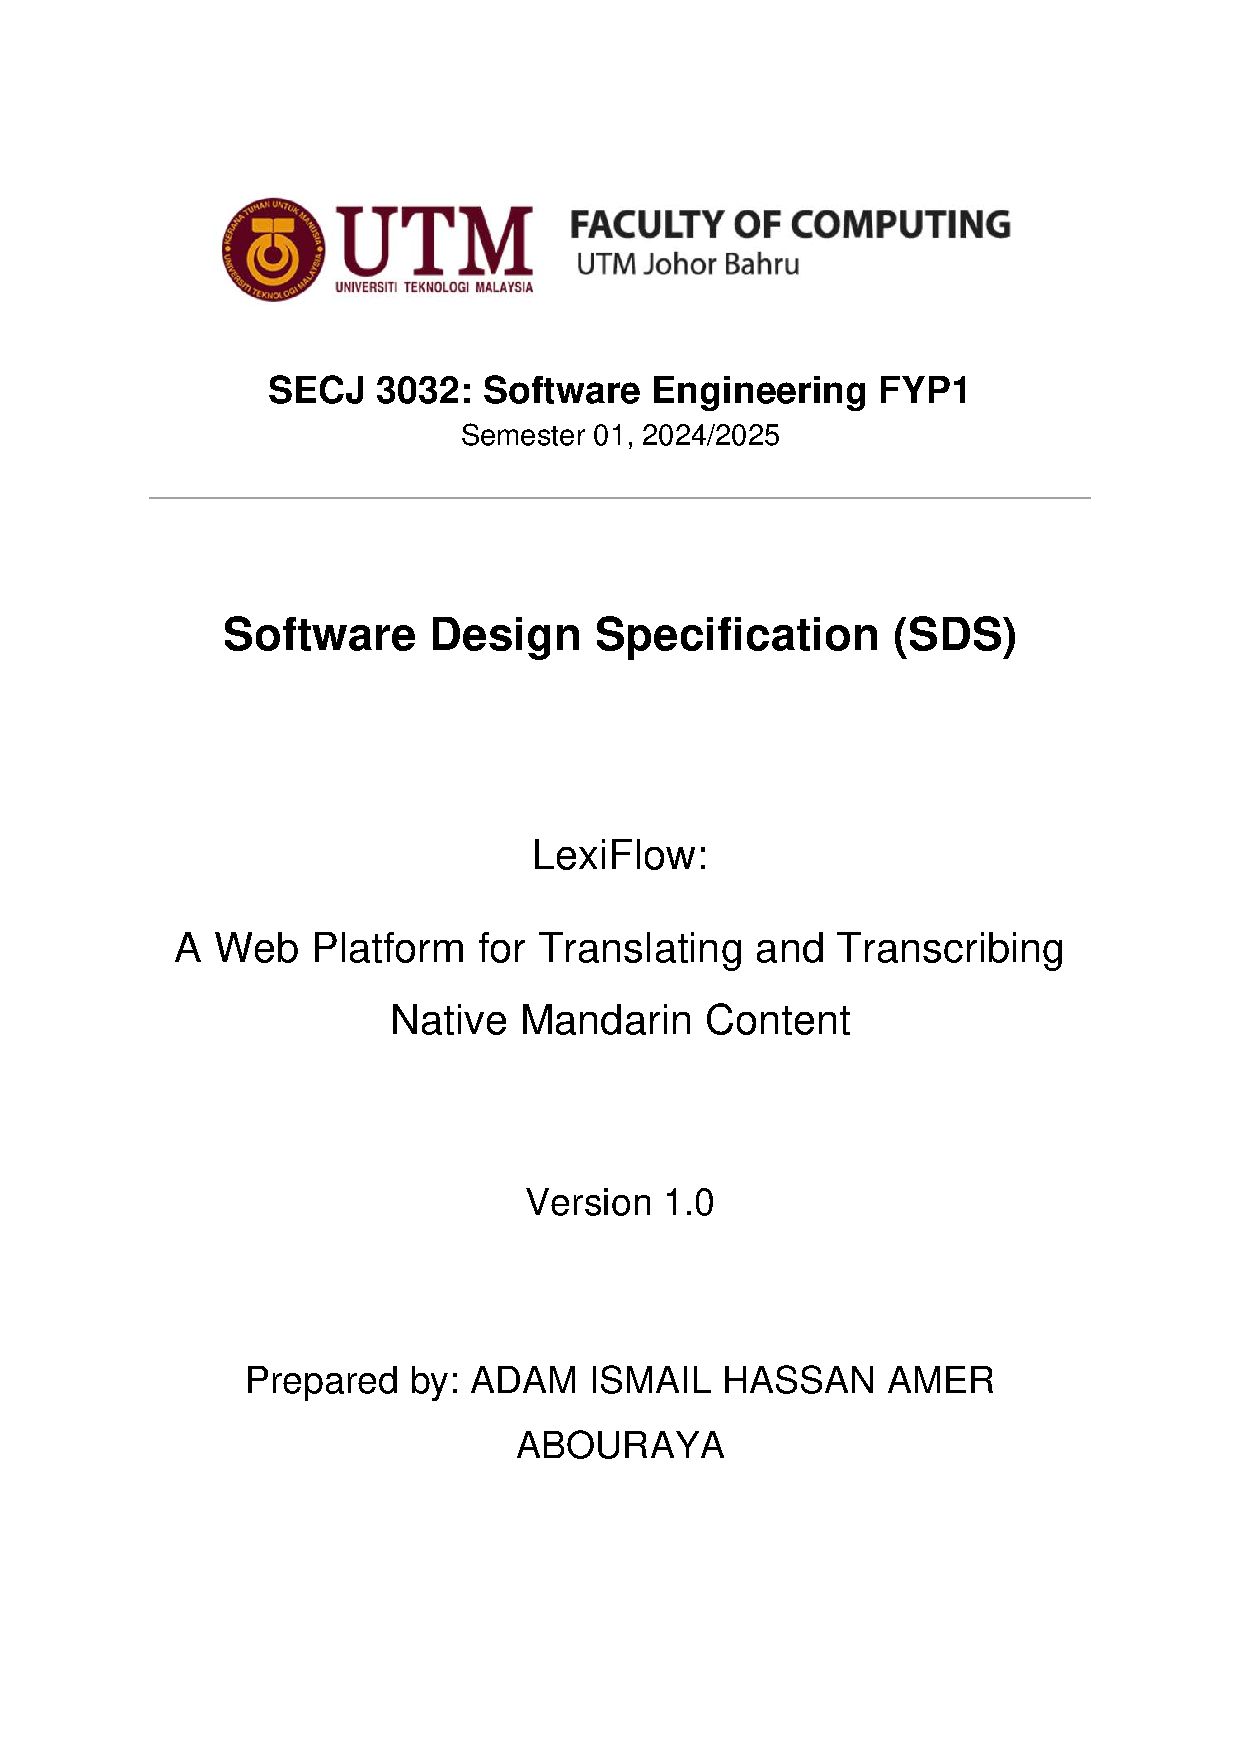
\includepdf[pages=-]{figs/sdd.pdf}
% \hspace{\fill}


%This is required to make List of Appendices possible. Remove when have no appendix.
\endmatter
\end{document}
